%# -*- coding: utf-8-unix -*-
%%==================================================
%% thesis.tex
%%==================================================

\documentclass[master, fontset=adobe, openright, twoside, openany]{sjtuthesis}
% \documentclass[%
%   bachelor|master|doctor,	% 必选项
%   fontset=adobe|windows,  	% 只测试了adobe
%   oneside|twoside,		% 单面打印,双面打印(奇偶页交换页边距,默认)
%   openany|openright, 		% 可以在奇数或者偶数页开新章|只在奇数页开新章(默认)
%   zihao=-4|5 		% 正文字号:小四、五号(默认)
%   review	 		% 盲审论文,隐去作者姓名、学号、导师姓名、致谢、发表论文和参与的项目
%   submit			% 定稿提交的论文,插入签名扫描版的原创性声明、授权声明 
% ]

% 逐个导入参考文献数据库
\addbibresource{bib/thesis.bib}

\begin{document}

%% 无编号内容:中英文论文封面、授权页
%# -*- coding: utf-8-unix -*-
\title{基于农业物联网和多物理场仿真的智能温室监测与控制研究}
\author{高浩天}
\advisor{黄震宇副教授}
\defenddate{2016年12月17日}
\school{上海交通大学}
\institute{电子信息与电气工程学院}
\studentnumber{1140359026}
\major{仪器仪表工程}

\englishtitle{Greenhouse Monitor}
\englishauthor{\textsc{Gao Haotian}}
\englishadvisor{Associate Prof. \textsc{Huang Zhenyu}}
\englishschool{Shanghai Jiao Tong University}
\englishinstitute{\textsc{School of Electronics and Electric Engineering} \\
  \textsc{Shanghai Jiao Tong University} \\
  \textsc{Shanghai, P.R.China}}
\englishmajor{Instrument}
\englishdate{Dec. 17th, 2016}


\maketitle

\makeenglishtitle

\makeatletter
\ifsjtu@submit\relax
	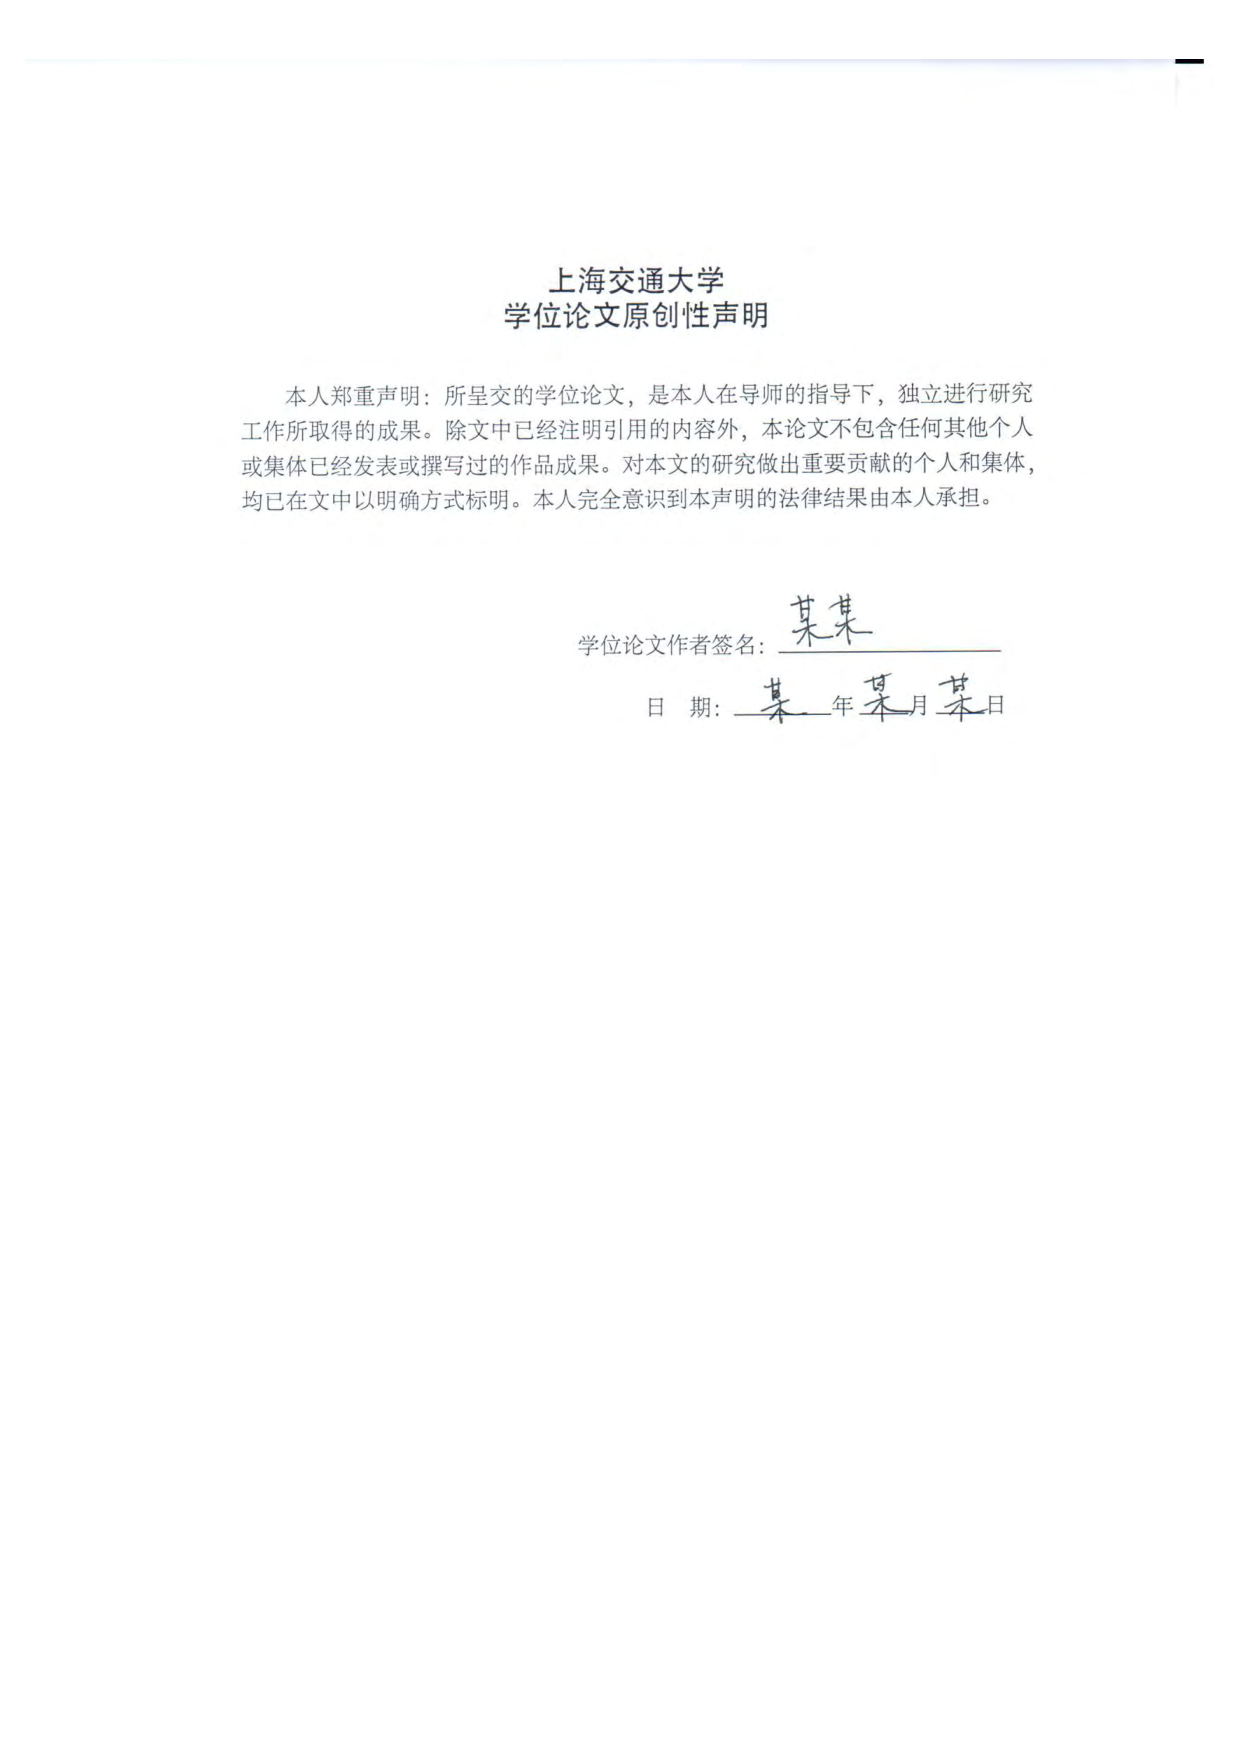
\includepdf{pdf/original.pdf}
	\cleardoublepage
	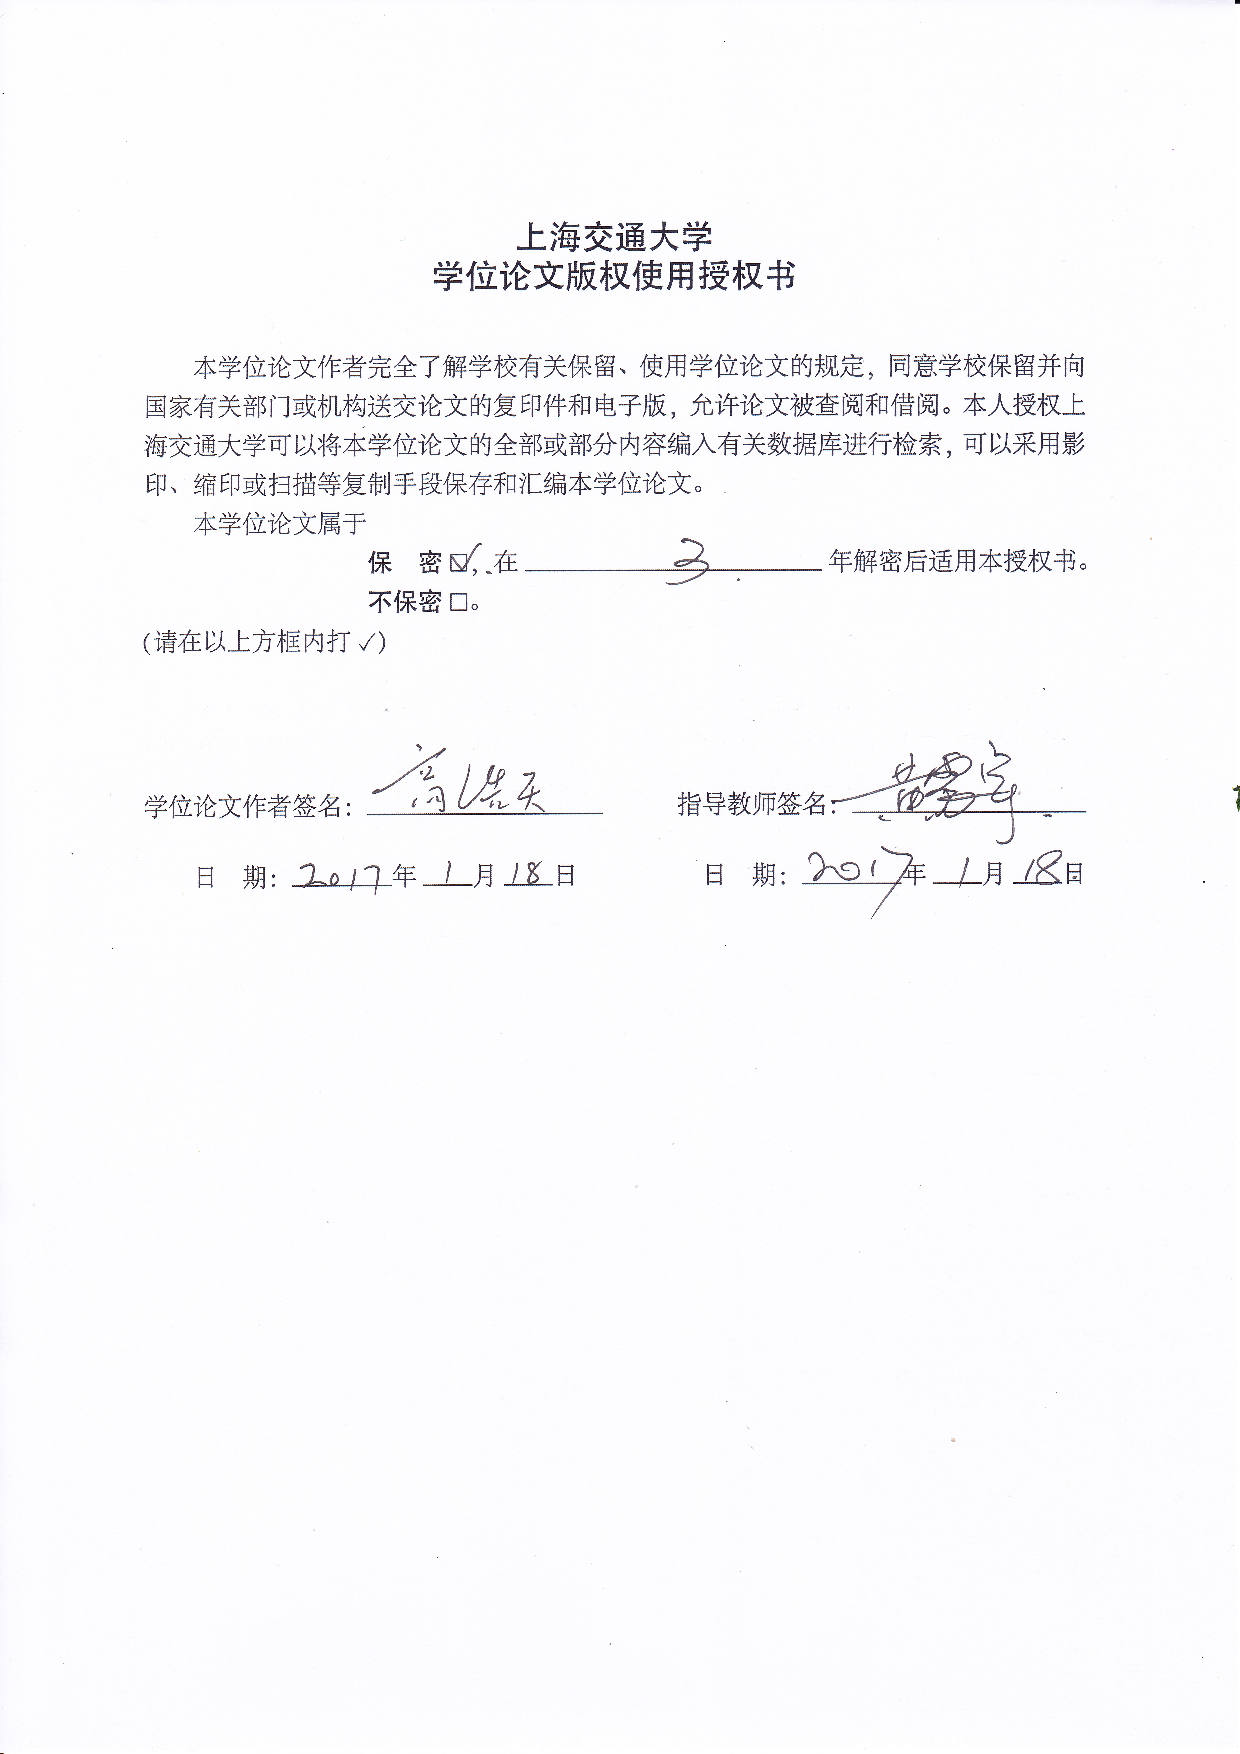
\includepdf{pdf/authorization.pdf}
	\cleardoublepage
\else
	\makeDeclareOriginal
	\makeDeclareAuthorization
\fi
\makeatother


\frontmatter 	% 使用罗马数字对前言编号

%% 摘要
\pagestyle{main}
%# -*- coding: utf-8-unix -*-
%%==================================================
%% abstract.tex for SJTU Master Thesis
%%==================================================

\begin{abstract}

农业物联网为农业生产环境的监控提供了新思路,可实现农业的智能化、信息化、精准化管理,是实现农业现代化的关键技术之一。基于农业物联网的智能温室系统,可通过网络监测温室环境,并根据作物的环境需求实施精准的温室控制,从而科学高效的管理温室。基于计算流体力学的温室仿真解决了复杂温室环境的建模分析问题,可以为智能温室系统的监测点位置优化和控制策略优化提供指导意见和理论依据。

通过分析温室监控的特殊需求并参考物联网标准架构,本文提出了基于农业物联网的智能温室架构方案。根据该架构设计了智能温室监测与控制系统:感知控制层基于ZigBee和RS485传感器网络及计算机控制模块,并针对可靠性、可扩展性、灵活性和低功耗进行了优化设计;网络传输层支持多种数据传输方式和数据同步机制,并针对网络传输的安全性、可靠性和高效性进行了重点设计,建立了系统层间枢纽;应用层包含数据中心、WEB服务器和智能策略学习控制子系统,提供了基于Hadoop和MySQL的海量温室历史数据的云存储解决方案,高可用免维护的云服务器和基于CFD仿真模型的优化控制策略;终端接入层采用WEB前端技术和React Native为系统提供了可视化界面。

智能温室监测与控制系统在实验温室进行了实测运行,运行结果表明:无线传感器网络稳定可靠,温室内外数据采集准确正常,上传同步延迟低,控制指令下达准确迅速,控制状态获取正常。数据中心工作正常,未发生慢查询或异常。云端WEB服务运行稳定,接口响应迅速,数据返回完整准确。系统满足预期设计要求和实际生产要求。

本文以南方地区典型的连栋塑料温室为研究对象,针对温室机械通风,建立了三维全尺度瞬态及稳态计算流体力学仿真模型。通过本文设计实现的智能温室监控系统,测量机械通风引起的温室内气温变化和分布,用实验验证了仿真模型瞬态和稳态计算的准确性和有效性。通过仿真模型模拟了室外高温条件下的风机数量、温室长度、入口温度及环境温度变化等参数对机械通风降温效果的影响程度,并模拟了不同数量风机启闭控制的降温效果。根据仿真分析结果优化了温室监测点位置方案和夏季机械通风控制策略。

经过对CFD仿真结果进行分析,优化后的温室监测点方案仅需最少5个监测点即可实现1280 $\text{m}^{2}$的温室整体环境状态的监测,有效减少了测点数量,降低了监测成本;优化后智能温室系统控制策略最高可减少约60\%的能源消耗,而植物冠层平均温度仅升高0.21℃,有效提高了机械通风降温效率,减少了能源消耗。

根据本文架构方案实现的智能温室监测与控制系统,节点布置灵活、监测范围广、运行功耗低、可靠性高、稳定性强、可灵活扩展,满足温室的智能和科学管理需求。结合CFD仿真分析,优化的监测点方案可有效降低监测成本,优化的机械通风控制策略可有效实现节能减排。系统还可实现异地温室集中互联,共同构建农业大数据和物联网平台,对农业科学研究和工程控制有重要意义,有助于提高农业现代化水平,推进农业物联网发展。

\keywords{\large 农业物联网 \quad 计算流体力学 \quad 温室 \quad 架构 \quad 监控系统}
\end{abstract}

\begin{englishabstract}

An imperial edict issued in 1896 by Emperor Guangxu, established Nanyang Public School in Shanghai. The normal school, school of foreign studies, middle school and a high school were established. Sheng Xuanhuai, the person responsible for proposing the idea to the emperor, became the first president and is regarded as the founder of the university.

\englishkeywords{\large SJTU, master thesis, XeTeX/LaTeX template}
\end{englishabstract}



%% 目录、插图目录、表格目录
\tableofcontents
\listoffigures
\addcontentsline{toc}{chapter}{\listfigurename} %将插图目录加入全文目录
\listoftables
\addcontentsline{toc}{chapter}{\listtablename}  %将表格目录加入全文目录
\listofalgorithms
\addcontentsline{toc}{chapter}{算法索引}        %将算法目录加入全文目录

%# -*- coding: utf-8-unix -*-
\chapter{主要符号对照表}
\label{chap:symb}

\begin{longtable}{rl}
$\epsilon$     & 介电常数 \\
 $\mu$ 		& 磁导率 \\
 $\epsilon$     & 介电常数 \\
\end{longtable}
 % 主要符号、缩略词对照表

\mainmatter	% 使用阿拉伯数字对正文编号

%% 正文内容
\pagestyle{main}
%# -*- coding: utf-8-unix -*-
%%==================================================
%% chapter0.tex for SJTU Master Thesis
%%==================================================


\chapter{绪论}
\label{chapter:Introduction}

\section{研究背景和意义}
自古以来,我们中国的祖先就知道“民以食为天”“粮食定,天下定”这一治国理政之道\supercite{ChenYunWenXuan},中国作为一个人口大国,解决全国人民的粮食食物问题是关系到国计民生的根本问题。根据农业科学院预测到2050年我国的人口将超过15亿,人口的大量增加也必然带来粮食需求量的猛增,要满足人口增长对粮食的需求,每年至少需要多生产1.2亿吨粮食。随着我国经济的飞速发展和人们生活水平的提高,人们不再仅仅关注于温饱的问题,更加追求品质生活,更加关注食品的安全、营养和多样\supercite{FengZhiming2007,ZhaoQiguo2011}。随之而来的,农业生产在不断扩大生产总量的同时也需要不断升级产业结构,以提供更加安全和高品质农副产品。

但是我国目前的农业生产的总体技术水平落后,现代化和信息化水平较低。农村的城镇化导致我国可用耕地面积不断减少,农村劳动力大量涌入城镇\supercite{YuJunli2001},务农人口急剧减少,农业生产人员逐步呈现老龄化和副业化趋势\supercite{LuoChaobin2005},传统的农业生产模式已经难以维持下去,这必然会促使农业生产者加大农药化肥产品的使用,食品安全受到前所未有的挑战,这与人民日益增长的对高品质安全食品的需求产生了难以消除的矛盾。同时随着中国市场的逐步开放,国内农产品市场与国际市场的竞争也在不断加剧。另一方面,我国还存在水资源紧缺、幅员辽阔但可用农业土地较少、生产能耗较高、基础设施建设不完善等问题。

为了解决这一系列问题,《国民经济和社会发展第十三个五年规划纲要》提出要推进农业现代化,并指出“农业是全面建成小康社会和实现现代化的基础,必须加快转变农业发展方式,着力构建现代农业产业体系、生产体系、经营体系,提高农业质量效益和竞争力,走产出高效、产品安全、资源节约、环境友好的农业现代化道路”,着重提出要推进农业物联网应用,提高农业信息化、智能化和精准化水平。

农业现代化的一个重要体现就是实现现代化的设施农业\supercite{LiuLei2013}。温室作为设施农业的重要组成部分,可以减少自然环境对于农业生产的限制,合理高效利用生产资源,人为地创造适宜的农业生产环境,提高农作物产量和质量,提高农业生产集约化程度。但是目前国内温室大多停留在电气化及以下水平,依靠农业生产者的经验对温室环境进行人工控制或电气化控制。已经实现的温室自动化监控系统多为本地监控,智能化和网络化程度较低,农业生产人员需要到现场才能获取相关数据,不便于生产应用和科学研究\supercite{duodiandapeng}。随着科技的发展进步,农业物联网为农业生产环境监控提供了新思路,通过物联网技术、传感器技术、互联网技术等先进的技术手段的综合运用可以实现农业环境的远程监测和控制,从而实现农业管理的智能化、网络化、综合化、多样化,是实现农业现代化的关键技术之一\supercite{JiYuWuLianWang,WuLianWang,ZhongGuoSheShiNongYe}。

本文课题来源于《现代农业装备与设施的研发》(沪农科攻字(2009)第8-1号),上海市2009科技兴农重点攻关项目,由上海市农业科学委员会主导并开展工作。随着今年来物联网技术、网络技术、云服务技术和智能终端的快速发展,本文综合运用物联网技术、无线传感技术和多物理场仿真技术等多领域前沿技术,设计并实现了一套基于物联网和计算流体力学仿真的智能温室监测与控制系统,该系统可远程监测和控制温室环境,让农业生产管理人员足不出户即可远程查看当前温室内的环境数据,通过视频查看当前温室内的实时情况,同时可通过远程操作温室内的作动器实现对温室内环境参数的控制。该系统还可结合种植作物的需求和当前温室内的实时环境根据智能化的温室自动控制策略实施精准的温室环境控制,从而科学高效的管理温室。消费者也可通过该系统了解到农作物的生产环境,一方面可以让消费者吃的安心放心,另一方面也可让消费者对农业生产进行监督,促进农业生产健康发展。
\section{国内外研究现状}
	\subsection{国内研究现状}
	我国是一个传统的农业大国,作为温室栽培的发源地,早在两千多年前就开始使用保护措施种植蔬菜。进入21世纪以来,我国的温室栽培技术得到快速提升,温室总面积不断增加,占据世界温室总面积的85\%以上,是温室栽培第一生产大国\supercite{WoGuoSheShiNongYe}。我国在现代温室方面的研究开始于20世纪30年代,日光温室首先在辽宁省应用于栽培蔬菜,随后我国从日本引进塑料薄膜技术开始中小拱棚的栽培,之后我国的温室一直处于发展缓慢的小规模低水平状态,直到上世纪70年代末,我国引进了一些国外的先进技术,我国的设施农业展开了新的篇章\supercite{xiandaiwenshi}。上世纪80年代开始,我国研究温室环境控制系统,并开始引入计算机控制,温室环境的控制效果得到了有效的改善\supercite{HanYi2016}。上世纪90年代后,我国在引进国外先进技术的基础上开始自主研制温室环境监控系统。上海交通大学、中国农业大学、中科院、农科院等科研院所和高校都研制出了具有不同特点的温室控制系统。
	
	经过多年的研究和时间,我国在现代温室方面的水平已经有了很大程度上的提高,但是在很多方面仍然落后于国际领先水平,主要体现在基础研究薄弱、设施结构不合理、装备和调控能力差、信息化和集约化程度低等方面\supercite{ZhangZhen2015,JiangWeijie2015} ,在温室环境的精准化、智能化控制等方面有较大的发展空间。
	\subsection{国外研究现状}
	美国、日本、荷兰等发达国家对于现代温室技术的研究起步较早,发展到今天,已经将计算机监控系统大规模应用到温室自动化生产中,在设备装备、环境控制和栽培技术等方面都处于国际领先水平。
	
	西欧是世界现代温室的发源地,虽然西欧国家的设施农业面积在世界世界设施农业总面积中占比不高,但是其现代化水平、生产质量和生产能力都非常高\supercite{GuoShirong2012}。荷兰是其中比较典型的设施农业非常发达的国家之一,主要对花卉和蔬菜进行专业化集约化生产,花卉和蔬菜出口量均居世界第一,有“欧洲菜园子”之称,其温室主要以玻璃温室为主,约占世界玻璃温室总面积的26\%以上\supercite{Watson,JiHong2007},农业生产的自动化程度很高,生产效率很高位居世界第一\supercite{QinLiu2015},其温室配套设备在满足内需的同时还大量出口到国外\supercite{Tavoletti2008Cutting}。
	
	美国的温室主要为连栋玻璃温室,现代化水平非常高。美国是最早将计算机技术投入到温室生产管理中的国家,通过政府的大力支持,采取了一系列的优惠政策,为农业现代化和信息化的发展创造了良好的氛围和环境。目前,美国约有82\%的温室采用计算机进行环境控制,27\%的农民还运用的网络技术\supercite{Kacira2011}。这样虽然提高了生产成本,但是也极大程度上给农业生产者带来了良好的经济效益\supercite{GuoShirong2012}。
	
	以色列是典型的中东国家,气候干旱,水资源匮乏,但是以色列的设施农业却非常发达,创造了沙漠中的片片绿洲,其开发的节水灌溉系统引入了计算机控制,可以精准控制水肥比例,处于世界领先水平,此外以色列对于作物生长机理的研究也比较深入,可据此建立合理的温室控制策略\supercite{GuoShirong2012,TangLibiao2003},主要生产高质量的花卉和果蔬,不仅可以自给自足还大量出口国外,享有”欧洲厨房“的美誉\supercite{QinLiu2015}。
	
	日本是一个资源非常匮乏的国家,且人口密度非常大,因此日本大力发展集约化、自动化的设施农业,主要生产果蔬和花卉,且依赖程度非常高\supercite{YangChunjun2010}。日本是最先提出植物工厂的概念,突破了土地和环境的限制,利用自动控制技术、电子技术、生物技术、机器人和新材料可以实现作物的全年连续生产,对于解决全球粮食问题和环境问题有着重要的现实意义\supercite{HuYongguang2002}。
	
	由此可见,发达国家在设施农业和现代化温室方面的研究处于非常明显的领先地位,在温室管理中大面积采用计算机控制系统,自动化和集约化程度都较高,目前正在向更为先进的智能化、精准化和网络化的方向发展。
\section{论文的主要内容与章节安排}
	\subsection{研究内容和创新点}
	本文结合物联网技术和计算力体力学仿真技术,对温室智能化监测与控制系统展开研究,主要有以下五部分内容:
		\begin{enumerate}
  			\item 适用于智能温室的农业物联网架构方案设计提出。
  			\item 针对温室机械通风三维全尺度瞬态及稳态计算流体力学仿真模型。
  			\item 针对南方地区典型的连栋塑料温室夏季机械通风实验与温室仿真模型验证。
  			\item 基于农业物联网的智能温室监测与控制系统的软件与硬件设计和实现。
  			\item 基于温室机械通风仿真模型的传感器测点位置选择与优化,及机械通风控制策略优化设计。
		\end{enumerate}
	相比于已有的相关研究,本文具有如下创新点:
		\begin{enumerate}
  			\item 本文根据农业生产环境的特殊性,通过分析温室监测与控制的特殊需求并参考物联网的标准框架,设计提出了一种适用于智能温室的农业物联网架构方案。设计并实现了基于该架构方案的智能温室远程监测与控制系统,并应用与连栋塑料温室,实现了对温室的智能感知、远程控制和智能控制,具有可靠性高、监测范围广、可灵活扩展、运行功耗低的优点,满足温室的智能运行和科学管理需求。
  			\item 为了解决我国南方地区夏季长期高温的恶劣天气对温室作物生长的严重影响,提高降温效果且减少通风能耗,本文以南方地区典型的连栋塑料温室为研究对象,针对温室机械通风,建立了三维全尺度瞬态及稳态计算流体力学仿真模型,研究了机械通风条件下温室内的气温变化和分布规律。通过在本文智能温室监测与控制系统平台上进行机械通风实验,验证了仿真模型瞬态和稳态计算的准确性和有效性。通过仿真模型模拟了室外高温条件下的风机数量、温室长度、入口温度和环境温度变化等参数对机械通风降温效果的影响程度,并模拟了不同数量风机启闭控制的降温效果,为智能温室监测和控制系统提供了优化的夏季机械通风控制策略,同时提供了优化的传感器测点布置策略,实现了以少量传感器测点数据准确反映大型温室气温分布。
		\end{enumerate}	
	\subsection{章节安排}
	本文的章节结构安排如下:
	
	第一章,绪论。介绍了本文课题的研究背景和研究意义、国内外在设施农业和现代化温室方面的研究进展和发展趋势、本文的主要研究内容和章节安排。
	
	第二章,基于农业物联网的智能温室架构。介绍物联网,提出基于农业物联网的智能温室四层架构方案,并对每层结构进行阐述和设计。
	
	第三章,智能温室监测与控制系统。详细介绍了基于本文农业物联网智能温室架构方案结合实际应用的具体实现,包括各层的硬件和软件实现。
	
	第四章,温室计算流体力学仿真及验证。基于计算流体力学建立三维全尺度瞬态及稳态机械通风仿真模型,利用本文智能温室监测与控制系统进行机械通风实验,并通过实验结果对仿真模型进行了验证。
	
	第五章,智能温室的实践与应用。详细介绍本文所设计实现的智能温室远程监测与控制系统在温室现场的实践与应用,以及温室仿真模型在实际应用中对于传感器测点位置选择优化作用和对温室机械通风控制策略的优化设计。
	
	第六章,总结与展望。总结研究内容,展望研究内容的发展前景和改进方向。 %绪论
%# -*- coding: utf-8-unix -*-
%%==================================================
%% chapter0.tex for SJTU Master Thesis
%%==================================================


\chapter{绪论}
\label{chapter:Introduction}

\section{研究背景和意义}
随着我国经济的飞速发展和国民生活水平的提高,人们不再只关注于温饱问题,更加追求生活质量,更加关注食品的品质、安全、营养和多样。随之而来的,农业生产在不断扩大生产总量的同时也需要不断升级产业结构,以提供更加安全和高品质农副产品。

然而我国目前的总体农业生产技术水平落后,现代化和信息化程度较低。农村的城镇化发展致使我国可用耕地面积逐渐减少,农村劳动人口大量涌入城镇,务农人员急剧减少,农业生产人员逐步呈现老龄化和副业化趋势,传统的农业生产模式已经难以维持下去,这必然会导致农业生产者对农药、化肥的过量使用,食品安全和生产环境受到前所未有的挑战,这与人民日益增长的对高品质安全食品的需求及可持续发展产生了难以消除的矛盾。同时随着中国市场的不断开放,国内农产品市场与国际市场的竞争也在不断加剧。另一方面,我国还存在水资源紧缺、幅员辽阔但可用农业土地较少、生产能耗较高、基础设施建设不完善等问题。

为了解决这一系列问题,“十三五规划”提出要推进农业现代化,转变农业发展方式,着重提出要推进农业物联网应用,提高农业信息化、智能化和精准化水平。

实现现代化的设施农业是推进农业现代化发展的重要途径。温室作为设施农业的重要组成部分,可以减少自然环境对于农业生产的限制,合理高效利用生产资源,通过人工的方式创造适宜的农业生产环境,提高农作物产量和质量,提高农业生产集约化水平。但是目前国内温室大多停留在电气化及以下水平,依靠农业生产者的经验对温室环境进行人工控制或电气化控制。已经实现的温室自动化监控系统多为本地监控,智能化和网络化程度较低,农业生产人员需要到现场才能获取相关数据,不便于生产应用和科学研究。随着技术的发展进步,农业物联网为温室环境监控提供了新的思路,通过物联网技术、感知控制技术、互联网技术等先进的技术手段的综合运用可以实现基于网络的温室环境监测和控制,从而实现温室的科学管理。

随着近年来物联网技术、网络技术、云服务和智能终端的快速进步,使基于物联网的智能温室监测与控制成为可能。但是农业生产面积大、投入成本有限、基础设施不完善、环境比较恶劣、不易值守,与传统物联网相比有其特殊的需求,需要对其感知控制层和网络传输层部分进行特殊的设计。同时由于温室内环境是一个流场、温度场、湿度场等多个物理场耦合在一起的多输入多输出的复杂大时延系统,对于温室的精准控制和监测需要借助计算流体动力学(Computational Fluid Dynamics,CFD)对温室环境的分布和变化过程进行分析。

本文综合运用物联网技术、无线网络技术和CFD仿真技术等多领域前沿技术,设计并实现了基于农业物联网的智能温室监测与控制系统,该系统可远程监测和控制温室环境,让农业生产管理人员足不出户即可远程查看当前温室内的环境数据,通过视频查看当前温室内的实时情况,同时可通过远程操作温室内的作动器实现对温室内环境参数的控制。该系统还可结合种植作物的需求和当前温室内的实时环境,根据经过已验证的温室CFD仿真模型和机器学习模型优化的智能化的温室自动控制策略,实施精准的温室环境控制,从而科学高效的管理温室。消费者也可通过该系统了解到农作物的生产环境,一方面可以让消费者吃的安心放心,另一方面也可让消费者对农业生产进行监督,促进农业生产健康发展。

\section{国内外研究现状}
	\subsection{国内研究现状}
进入21世纪以来,我国的温室栽培技术得到快速提升,温室总面积不断增加,占据世界温室总面积的85\%以上,是温室栽培第一生产大国。
	
我国在现代温室方面的研究开始于20世纪30年代,日光温室首先在辽宁省应用于栽培蔬菜,随后我国从日本引进塑料薄膜技术开始中小拱棚的栽培,之后我国的温室一直处于发展缓慢的小规模低水平状态,直到上世纪70年代末,随着一批国外先进设施农业技术的引入,我国的设施农业展开了新的篇章。上世纪80年代开始,我国对温室环境监控系统开展研究,并开始引入计算机控制,温室环境的控制效果有了明显的改善。上世纪90年代后,通过对国外先进技术的吸收消化,我国开始自主研制温室环境监控系统。上海交通大学、中国农业大学、中科院、农科院等科研院所和高校都研制出了具有不同特点的温室监控系统。

经过多年的研究和实践,我国在现代温室方面的水平已经有了很大程度上的提高,但是在很多方面仍然落后于国际领先水平,主要体现在基础研究薄弱、设施结构不合理、装备和调控能力差、信息化和集约化程度低等方面,在温室环境的精准化、智能化监控等方面有较大的发展空间。

	\subsection{国外研究现状}
美国、日本、荷兰等发达国家对于现代温室技术的研究起步较早,发展到今天,已经将计算机监控系统大规模应用到温室自动化生产中,在设施装备、环境调控和栽培技术等方面都处于国际领先水平。
	
西欧是世界现代温室的发源地,虽然西欧国家的设施农业面积在世界总面积中占比不高,但是其现代化水平、生产质量和产量都非常高。荷兰是其中比较典型的设施农业非常发达的国家之一,主要对花卉和蔬菜进行专业化集约化生产,且出口量都为世界首位,有“欧洲菜园子”之称,其温室主要以玻璃温室为主,在世界玻璃温室总面积中占比26\%以上,农业生产的自动化程度很高,且效率很高,位居世界第一,其温室配套设备在满足内需的同时还能够出口很多到国外。

美国的温室主要为大型玻璃温室,现代化程度非常高。美国是最早将计算机技术投入到温室生产管理中的国家,通过政府的大力支持,采取了一系列的优惠政策,为农业现代化和信息化的发展创造了良好的氛围和环境。目前,美国约有82\%的温室环境通过计算机进行控制,27\%的农民还运用了网络技术。这样虽然提高了生产成本,但是也极大程度上给农业生产者带来了良好的经济效益。

以色列是典型的中东国家,气候干旱,水资源匮乏,但是以色列的设施农业却非常发达,创造了沙漠中的片片绿洲,其开发的节水灌溉系统引入了计算机控制,可以精准控制水肥比例,处于世界领先水平,此外以色列对于作物生长机理的研究也比较深入,可据此建立合理的温室控制策略,主要生产高质量的花卉和果蔬,不仅可以自给自足还大量出口国外,享有“欧洲厨房”的美誉。

日本是一个资源非常匮乏的国家,且人口密度非常大,因此日本大力发展集约化、自动化的设施农业,主要生产果蔬和花卉,且依赖程度非常高。日本最早提出植物工厂的概念,突破了土地和环境的限制,利用先进的技术手段可以实现作物的全年不中断生产,对于世界农业发展有着重要的现实意义。

由此可见,发达国家在设施农业和现代化温室方面的研究处于非常明显的领先地位,在温室管理中大面积引入计算机控制,自动化和集约化水平都较高,目前正在向更为先进的智能化、精准化和网络化的方向发展。

\section{农业物联网简介}
	\subsection{物联网概念}
1995年,比尔·盖茨在《The Road Ahead》中最早提及了Internet of Things一词,但是受限于当时的网络技术、传感器技术和智能硬件技术的发展,并没有引起广泛的关注和重视。2005年国际电信联盟(International Telecommunication Union,ITU)在《ITU Internet Report 2005: The Internet of Things》中正式提出了“物联网”的概念。
	
	\begin{figure}[!htp]
  		\centering
 		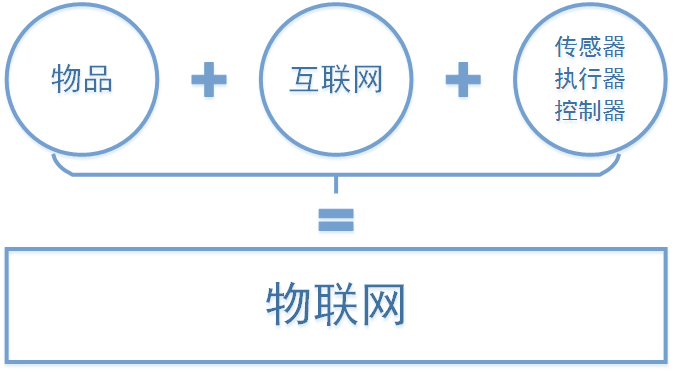
\includegraphics[width=0.5\textwidth]{01CompositionIoT.png}
  		\bicaption[fig:CompositionIoT]{物联网的基本构成}{物联网的基本构成}{Fig}{Composition of the Internet of Things}
	\end{figure}
	
为了解释物联网这一概念,首先要了解这个词是如何被创造的,物联网之父Kevin Ashton曾指出,互联网中的大部分数据都是通过人为的控制进入系统中的,在系统中,人所充当的角色无非是一种效率低下、易出错、对数据的数量和质量有所限制的路由器,并在一定的情况下可以对数据进行解释和修正,但是从另一个角度如果系统能够抛开人的限制直接连接到互联网,通过传感器获取现实世界的数据并对现实世界进行一定的控制,这样会变得更加高效、丰富和准确。物联网也即是万物相连的互联网,我们连接物体所获得的一切都是由互联网和物体自身控制,而非人。因此,物联网是建立在互联网的基础之上的,是互联网的延伸和拓展,而信息的获取和交换从人为控制扩展到了物和物之间自主进行。我们可以用一个非常简单的组成关系来描述物联网的基本构成,如\ref{fig:CompositionIoT}所示。
	
	\subsection{物联网的特征及内涵}
根据物联网的概念、物联网和互联网的异同,结合国内外专家的解释,物联网具有如下的特征和内涵:
	\begin{enumerate}
  		\item 物联网系统中包含大量各式各样的传感器,它们都担任着连接万物的使命,连续不断的获取和更新外界的实时数据。
  		\item 物联网并不是一种全新的信息传递网络,其通过各种有线或者无线网络接入互联网进行物体信息的实时传递,实现世间万物包括人之间的实时交互,最终达到为人服务的目的。
  		\item 物联网自身也是一个智能系统,它不仅可以通过传感器获取数据,同样也具备智能分析处理的能力,对数据进行清洗筛选得到有意义的数据,然后通过控制器和执行器对物体进行智能控制。
  		\item 物联网即是未来的互联网。我们希望实现的不仅仅是物与物的局部信息传递,而是最终要实现所有的人和世间万物的互连互通,这也与未来的互联网的发展趋势是一致的。
	\end{enumerate}
	
	\subsection{物联网在农业中的应用}
“十三五”规划纲要指出要加速新一代的信息基础设施建设,推进信息网络技术广泛运用,形成万物互联、人机交互、天地一体的网络空间,加快物联网基础的布局,将物联网应用在社会生活的各个方面。同时指出要推进农业现代化建设,推进农业物联网和农业大数据的实践应用,提高农业生产的智能化和精准化水平。随着物联网技术的不断发展,农业的现代化、智能化和信息化发展迎来了新的解决方案和发展机遇。
	
目前,物联网技术在工业领域已经得到了较为广泛的应用,但是农业领域的物联网应用还处在研究发展阶段。近年来,欧美等发达国家陆续开展了农业物联网的相关工作研究,并进行了一系列的实践推广,推动了农业物联网的发展。我国也在农业物联网相关方面开展了积极的研究工作,主要实现农业生产环境资源的信息互通共享,以及农产品生产和物流等过程中的信息采集和通信,形成产前合理规划提高资源利用率,产中现代化管理提高生产效率、安全生产、节约成本提高效益,产后高效流通和安全溯源的农业物联网一条龙解决方案,但是产品多处于试验阶段,产品的稳定性、可靠性、低功耗等性能参数上与国际领先的产品还存在一定的差距。因此我国的农业物联网相关研究工作还有很大的发展空间。
	
	\subsection{农业物联网的特点}
农业的生产环境和工业环境相比,有其自身的特点和限制,这也决定了农业物联网所处的物理环境和网络条件与工业物联网有着本质的区别。因此农业物联网有其自己的特点和特殊需求,主要有如下几点:
	\begin{enumerate}
  			\item 成本有限,布点稀疏。农业生产的单位收益不高,投入成本有限,此外,大面积在农业生产环境内布置传感器测点会给农业作业,尤其是农业机械化作业带来干扰,这就决定了农业物联网中不可能密集布置传感器测点。因此,农业物联网在农业生产环境中应用时,往往布置稀疏的传感器测点。这就要求农业物联网具有远距离传输和灵活扩展的能力。
  			\item 环境复杂,不易值守。农业物联网工作环境往往面积较大且地形复杂,不易于值守,也无市电供电。因此,在要求各节点具有远距离传输能力的同时还要求功耗尽量小,能够依靠环境能源实现长期不间断的工作。
  			\item 环境恶劣,易受干扰。农业生产环境恶劣,设备经常长时间工作在高温、高湿、低温等极端环境下,且在进行无线通信时易受作物植被的干扰,这就对农业物联网设备的稳定性、可靠性、自诊断和免维护能力提出了要求。
  			\item 实时性要求相对较低。相比工业生产,农业环境变化缓慢,因此农业生产实时性要求不高。
	\end{enumerate}


\section{论文的主要内容与章节安排}
	\subsection{研究内容和创新点}
本文结合农业物联网技术和计算流体动力学仿真技术,对温室智能化监测与控制系统展开研究,主要有以下五部分内容:
		\begin{enumerate}
			\item 基于农业物联网的智能温室架构方案设计提出。
			\item 智能温室监测与控制系统的软件与硬件设计和实现。
			\item 针对温室机械通风三维全尺度瞬态及稳态计算流体动力学仿真模型。
			\item 针对南方地区典型的连栋塑料温室夏季机械通风实验与温室仿真模型验证。
			\item 基于温室机械通风仿真模型的传感器测点位置选择与优化,及机械通风控制策略优化设计。
		\end{enumerate}
		
相比于已有的相关研究,本文具有如下创新点:
		\begin{enumerate}
			\item 通过分析温室监控需求并参考物联网通用架构,设计提出了一种适用于温室监控的智能温室架构。设计并实现了基于该架构方案的智能温室远程监测与控制系统。根据农业生产的特点,构建了可灵活布点的无线传感网络,自定义了网络通信流程协议,进行了节点低功耗设计;使用生产者消费者设计模式解决监测数据丢包;通过数据库二进制日志文件订阅解决了数据库异地同步;搭建了海量温室数据分布式存储系统。实现了对温室的智能感知、远程和智能控制,具有可靠性高、稳定性强、监测范围广、可灵活扩展、运行功耗低的优点。
			\item 针对南方地区典型的连栋塑料温室机械通风,建立并验证了三维全尺度瞬态及稳态计算流体动力学仿真模型,耦合了流场、温度场、湿度场等多个物理场,研究了机械通风条件下温室内的空气温度变化和分布规律。
			\item 通过仿真模型模拟了室外高温条件下的风机数量、温室长度、入口温度和环境温度变化等参数对机械通风降温效果的影响程度,并模拟了不同数量风机启闭控制的降温效果,为智能温室监测和控制系统提供了优化的夏季机械通风控制策略,有效降低了夏季温室的机械通风降温能耗,同时提供了优化的传感器测点布置策略,以少量监测点数据准确反映大型温室环境分布。此外,还可以在温室设计阶段优化温室结构参数和设备配置。
		\end{enumerate}	
	\subsection{章节安排}
	本文的章节结构安排如下:
	
第一章,绪论。介绍了本文课题的研究背景和研究意义、国内外在设施农业和现代化温室方面的研究进展和发展趋势、本文的主要研究内容和章节安排。

第二章,基于农业物联网的智能温室架构。分析智能温室系统在各个方面的需求,提出基于农业物联网的智能温室四层架构方案,并对每层结构进行阐述和设计。

第三章,智能温室监测与控制系统。详细介绍了基于本文农业物联网智能温室架构方案结合实际应用的具体实现,包括各层的硬件和软件实现。

第四章,温室计算流体力学仿真及验证。基于计算流体力学建立三维全尺度瞬态及稳态机械通风仿真模型,利用本文智能温室监测与控制系统进行机械通风实验,并通过实验结果对仿真模型进行了验证。

第五章,智能温室的实践与应用。详细介绍本文所设计实现的智能温室远程监测与控制系统在温室现场的实践与应用,以及温室仿真模型在实际应用中对于传感器测点位置选择优化作用和对温室机械通风控制策略的优化设计。

第六章,总结与展望。总结研究内容,展望研究内容的发展前景和改进方向。 %基于农业物联网的智能温室架构
%# -*- coding: utf-8-unix -*-
%%==================================================
%% chapter1.tex for SJTU Master Thesis
%%==================================================

\chapter{基于农业物联网的智能温室架构}
\label{chapter:IoT Architecture}
农业生产环境有其自身的特点,智能温室也有其特殊的应用需求,在对智能温室的各方面需求进行分析之后,结合通用物联网的层次结构,本章提出了基于农业物联网的智能温室系统的四层架构,并对架构中的每一层进行了概要设计。

\section{智能温室需求分析}
	\subsection{温室环境感知}
智能温室的关键功能即实现对温室环境的实时全面感知。为了保证温室内作物的正常生长,至少需要对室内的空气温湿度、土壤温湿度和光照等参数进行采集\supercite{ZhouTao2015};为了对温室内环境参数进行控制,还需要对室外的空气温湿度、风速、风向、太阳辐射强度和降雨量等对温室环境有直接影响的参数进行采集。为了同时满足生产和科研的需要,数据采集需要可以灵活配置采样频率。由于温室面积一般较大,且不同的温室结构不尽相同,因此需要感知网络节点可以灵活扩展和部署。农业生产的环境恶劣、基础设施落后和不易值守等特点决定了节点必须具有高稳定性、高可靠性、免维护性、低功耗性等特点。
	\subsection{数据传输与同步}
数据传输是系统各部分之间的纽带,安全、稳定、可靠、高效的数据传输与同步是系统正常工作的重要保证,智能温室对于温室数据的传输与同步提出了如下几点要求:
		\begin{enumerate}
			\item 安全性。数据不仅包括温室环境数据等的传出,还包括温室控制指令等数据的传入,为了保证设备的安全运行,避免恶意操作导致安全事故,必要保证数据传输的网络安全。
			\item 可靠性和稳定性。智能温室需要全天候地获取温室实时环境数据以根据控制策略对温室内作动器进行合理的控制,还需要保证控制指令能够准确无误地下达到温室控制器,因此必须保证系统数据传输的稳定可靠,以确保温室环境数据能够准确稳定地上传同步,控制指令能够正确可靠地下达。
			\item 高效性。虽然温室环境数据变化相对缓慢,对于实时性要求不高,但是对于温室控制如果控制指令不能及时传输下发到控制器,有可能会导致设备损坏,因此系统对于数据传输有一定时效性的要求。温室视频监测更加要求数据传输网络快速高效。	
		\end{enumerate}

	\subsection{海量数据存储}
温室监测需要全天候不间断的进行数据采集,这将带来海量的监测数据,同时智能温室系统还伴随着大量的控制日志记录和其它相关日志记录,海量数据给存储系统提出了较高的要求\supercite{SunHongying2010}。首先是对数据容量的要求,存储容量不仅要满足近期的数据存储,还需要能够灵活扩容;然后是对存储性能的要求,在数据量不断增加的情况下需要系统能够保证系统性能,避免出现慢查询、操作执行缓慢等现象;最后是对数据安全性的要求,系统长期记录积累的数据对农业生产管理和科学研究有着重要的意义,如果出现数据丢失或损坏将是一项重大的损失,因此要求系统有完善的灾备和恢复能力。
	\subsection{智能控制}
温室系统的智能控制部分相当于整个系统的大脑,代替温室生产管理人员对温室进行控制,将人从温室农业生产中解放出来。智能控制部分不仅需要汲取农业生产者和专家的经验作为先验知识生成初始的控制策略,还需要后期可以对控制策略进行灵活的升级,最后还对智能控制的自我学习能力提出了要求,系统能够不断通过历史数据的分析挖掘、仿真系统的计算优化,自主地更新当前的控制策略,实现系统的迭代更新。
	\subsection{应用程序与数据访问}
智能温室最终是为人类和农业生产服务,因此必须拥有友好的数据访问,开发功能丰富的应用程序,能够让用户方便快捷、科学高效地监测和管理温室。作为基于农业物联网的系统,要求系统不仅需要对用户友好,还需要对其它物联网设备和系统友好,使其它设备和系统能够轻松地接入智能温室系统,共同组建完善的生态系统。


\section{系统整体架构设计}
	\subsection{物联网通用层次定义}
	根据一般的物联网架构层次定义\supercite{Yu2011,LiuQiang2010} ,物联网可分为感知层、网络层和应用层三层结构\supercite{HanYi2016A,WangHuaiyu2015} ,如图\ref{fig:ArchitectureIoT}所示。
	
	\begin{figure}[!htbp]
  		\centering
 		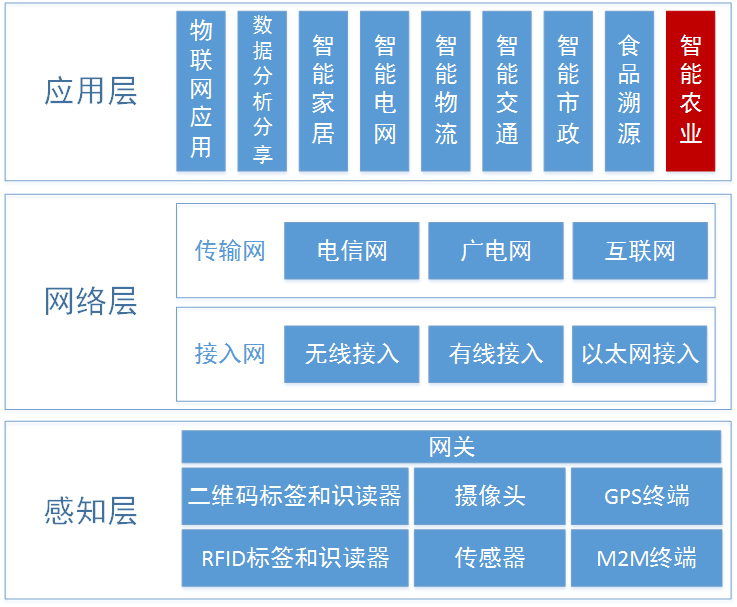
\includegraphics[width=0.5\textwidth]{02ArchitectureIoT.png}
  		\bicaption[fig:ArchitectureIoT]{物联网层次架构}{物联网层次架构}{Fig}{Architecture of the Internet of Things}
	\end{figure}
	感知层是物联网的核心部分,位于物联网三层结构的最接近物的一层,是信息采集的关键部分,是架设在人与物之间的桥梁,主要负责物联网系统的“感知”,相当于人类五官的功能,包含各种传感器和传感器组成的网络两部分,可以对物体的各类属性和环境状态等数据信息进行动态感知、快速识别和持续采集。该层的发展主要依赖于近场通信技术、传感器技术、网络技术和现场控制技术的发展。
	
网络层是物联网的枢纽部分,位于物联网三层结构中的中间层,是信息传输的重要枢纽,其功能为通过搭建起的通信网络进行各种信息传输。网络层承担着连接感知层和应用层的重任,主要用于将物联网底层所捕获到的信息,根据不同的应用需求进行一定的信息处理,然后安全、稳定、可靠地传输到上层应用。网络层分为两种网络,一种是负责底层传感器网络等接入的接入网,可以通过各类有线或者无线的方式接入;另一种是负责信息传输的传输网,包括互联网、大型局域网等。总而言之,网络层中运用各种网络形式,最终实现万物互联的目的。

应用层是物联网的最顶层,主要负责各种信息处理\supercite{DengMiwen2015}。应用层和感知层是物联网最核心的部分,应用层通过对感知层捕获的信息进行分析和处理,从而实现对万物的全面感知和科学控制。目前,其核心功能主要围绕数据的管理与处理,以及数据与各行业应用相结合。应用层主要包括智能家居、智能电网、智能农业等。应用层是物联网与用户接触最紧密的一层,用户所能感受到的各种具体的服务和应用都是由应用层所提供的,同时应用层又是目前发展相对滞后的一层,因此应用层还有很大的发展空间和潜力。

	
	\subsection{智能温室整体架构设计}
本文设计的基于农业物联网的智能温室系统由底向上划分为感知控制层、网络传输层和应用层,符合物联网的通用层次定义,另外为了兼容各类终端和系统的接入添加了终端接入层\supercite{WangHuaiyu2015} ,如图\ref{fig:System}所示。

	\begin{figure}[!htbp]
		\centering
		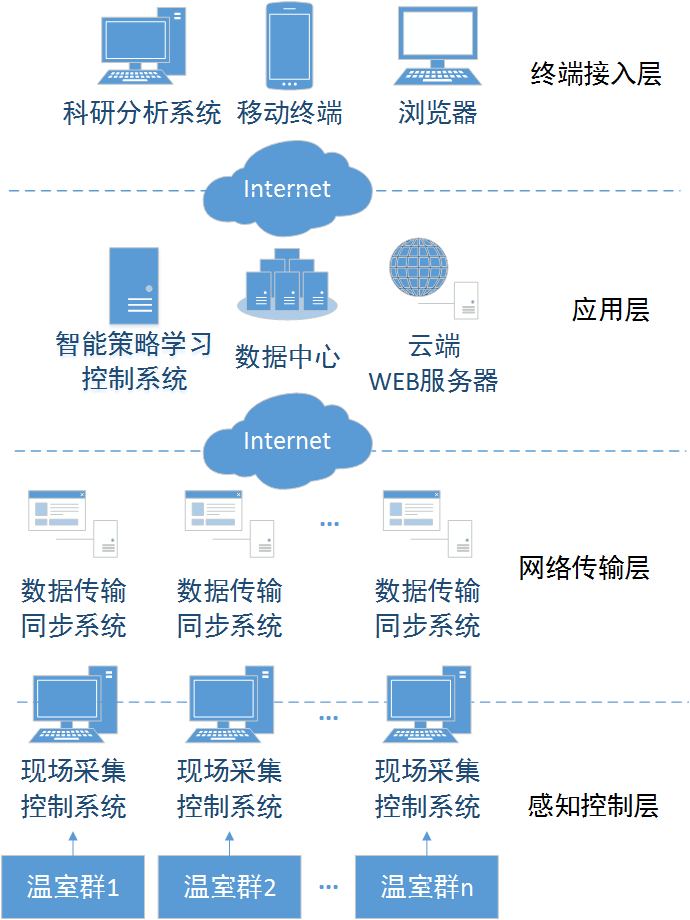
\includegraphics[width=0.5\textwidth]{03ArchitectureSystem.png}
		\bicaption[fig:System]{智能温室系统整体架构}{智能温室系统整体架构}{Fig}{Architecture of the intelligent greenhouse system.}
	\end{figure}	
\section{感知控制层}
感知控制层主要用于获取需要监测及用于控制的各类温室环境参数数据,以及对温室现场的作动器进行控制以达到控制温室内环境参数的目的。本层通过现场采集控制系统实现,其总体设计如图\ref{fig:Sensing}所示。针对农业特殊的生产环境,本层适合使用可靠性高、稳定性强、灵活性大、易于扩展的传感器网络采集温室环境参数数据,如基于RS485总线的有线传感器网络、基于ZigBee的无线传感器网络等。

	\begin{figure}[!htbp]
		\centering
		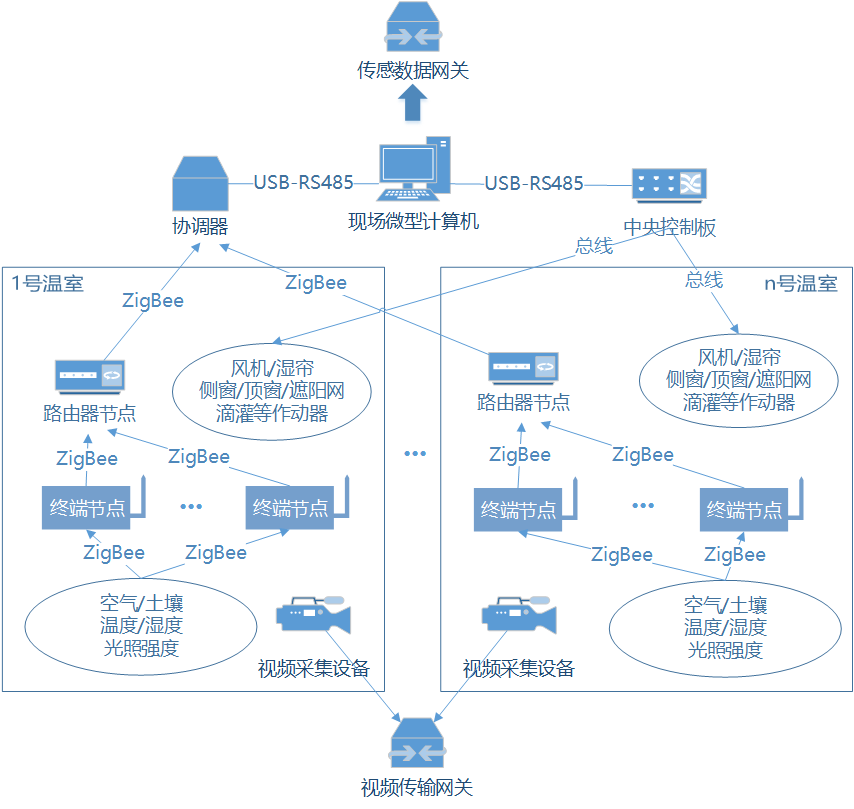
\includegraphics[width=0.7\textwidth]{04Sensing.png}
		\bicaption[fig:Sensing]{智能温室系统整体架构}{智能温室系统整体架构}{Fig}{Architecture of the intelligent greenhouse system.}
	\end{figure}

监测到当前温室环境后,系统需要通过控制温室内作动器的动作对温室内的环境加以控制,从而达到让温室环境更加适宜温室内作物生长的目的。因此本层还包括用于控制温室内作动器的中央控制板。为降低成本的同时提高设备的可靠性,本系统适合采用嵌入式计算机提供现场计算服务,同时兼用作网关服务,如基于ARM的微型计算机等。另外,为了增加对温室内环境的直观感知,本层添加了图像采集模块,包括图像采集设备和图像传输网关,该模块可在需要视频或图像监测的温室内使用。
\section{网络传输层}
网络传输层主要负责温室环境参数监测数据的传输与同步,以及控制命令的下发,从而架设起感知控制层和应用层之间的桥梁,起到数据枢纽的作用。一方面用于将温室现场采集到的数据经过简单的清洗、处理和存储,然后将数据同步上传到上层系统。另一方面用于将上层系统下达的控制指令简单解析处理,然后下发到下层系统。

考虑到农业生产环境多处于城市郊区、农村等偏远地区,网络基础设施薄弱不完善,大部分地区甚至没有接入有线网络,这对网络层的网络传输提出了要求。本系统提供了多种方式接入互联网,从而与云端系统相连接,如GPRS、3G、4G、光纤网络、ADSL等,系统使用者可以通过任意方式接入互联网,使现场系统与云端系统相连接。

\section{应用层}
应用层提供智能温室远程监控系统的核心服务,由数据中心、WEB服务器和智能策略学习控制子系统三部分组成。

数据中心用于将下层系统上传的温室环境参数数据进行云端同步存储,并实现海量历史数据的存储;WEB服务器提供数据请求服务和控制请求服务;智能策略学习控制子系统为智能温室提供自动控制策略,并可以随时根据温室CFD模拟仿真结果优化更新控制策略,也可通过海量历史数据进行机器学习和数据挖掘,对温室环境控制策略机器学习模型进行自主训练,实现温室环境智能控制策略的自我学习与迭代更新。

\section{终端接入层}
 终端接入层主要是为了兼容各类设备的接入而添加的,如PC、各类智能移动设备、浏览器、科研分析系统等。该层提供友好的可视化界面,用户可对温室环境进行监测和对温室设备进行远程在线控制或选择控制策略。同时,本层提供历史数据导出服务,用户可远程导出任意历史数据用于管理决策和科研分析等。其它物联网系统也可通过该层接入本系统,共同构建更加丰富完整的农业物联网生态系统。
 
\section{本章小结}
本章对于智能温室的系统需求分析指出了智能温室在环境感知、数据传输同步、数据存储、智能控制、系统应用等方面的要求;然后阐述和分析了物联网的通用层次定义;最后针对分析所得需求,结合通用物联网的层次结构划分和农业物联网的特点,提出了基于农业物联网的智能温室系统的整体架构设计,共分为感知控制层、网络传输层、应用层和终端接入层,并对系统中的每一层进行了概要设计。 %智能温室监测与控制系统
%# -*- coding: utf-8-unix -*-
%%==================================================
%% chapter0.tex for SJTU Master Thesis
%%==================================================


\chapter{智能温室监测与控制系统}
\label{chapter:IntelligentGreenhouseSystem}
基于智能温室系统的四层架构设计和各层次的概要设计,本章分别对系统中的感知控制层、网络传输层、应用层和终端接入层进行了详细地设计与实现,并最终完成了智能温室监测与控制系统。

\section{感知控制层设计与实现}
	\subsection{传感器网络选择}
温室内应用环境特殊,通常可供布置传感器的空间有限、温室内种植植物导致布线困难、温室面积较大从而监测范围大、农业生产环境不易值守且维护不便,传统的有线传感器网络对于温室内环境的监测不是一个很好的选择\supercite{YangFan2008} 。针对温室内环境监测传感器布置困难、供电困难、搭建和维护成本限制大等因素,综合考虑,本系统对于温室内环境监测选用ZigBee无线传感器网络。

ZigBee技术是一种基于IEEE 802.15.4标准的局域网通信技术,是无线传感器网络(Wireless sensor networks, WSNs)信息采集系统的一个重要组成部分,主要用于传感测量和控制应用,具有低功耗、低成本、复杂度低、短延迟、高容量、高安全性、自组网、可灵活扩展、使用免执照频段等优良性能。

由于系统内室外环境监测使用的室外微型气象站和太阳辐射传感器安装部署位置固定,不存在温室内传感器测点所存在的问题,因此采用抗噪能力强、传输距离长、实现成本低的RS485有线传感器网络。

两种网络均通过USB转串口与上层系统连接通讯。
	\subsection{传感器网络硬件组成}
	温室内无线传感器网络有三种类型的设备组成,分别为终端节点、路由器节点和协调器\supercite{ZhouJianmin2011} 。各节点的硬件设计采用模块化设计,各功能模块独立设计,然后通过标准化的接口连接组合成完整的节点,这样既便于维护和升级,同时可以减少主板体积。一个完整节点主要包括核心板模块、传感器模块和底板,其中终端节点和路由器节点包含所有模块,协调器节点不包含传感器模块。
		\subsubsection{核心板模块}
		核心板由Texas Instruments公司的CC2530 SoC芯片、外围电路及天线组成,如图\ref{fig:CC2530}所示。CC2530是用于2.4GHz IEEE 802.15.4和ZigBee应用的片上解决方案,集成了一块增强型8051MCU和一块射频芯片,具有系统内可编程闪存和8-KB RAM、最大256KB的Flash;结合了TI在业内领先的高性能RF收发器,内置4个不同功能的定时器,高度集成的片上系统提供了丰富的外设,只需少量的外部器件即可开发丰富的应用,满足低功耗设计的需求,适用于温室的控制和测量。
		
		\begin{figure}[!htbp]
  			\centering
 			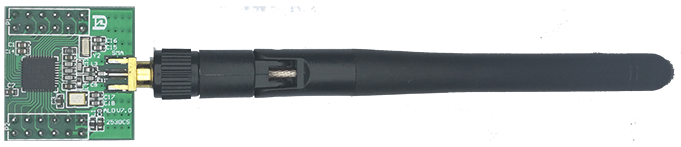
\includegraphics[width=0.5\textwidth]{05CoreBoard.png}
  			\bicaption[fig:CC2530]{CC2530核心板}{CC2530核心板}{Fig}{CC2530 core board}
		\end{figure}	
		核心板上主要包括CC2530F256单片机、天线接口、晶振、I/O扩展接口等,只需要提供2~3.6V的外部供电并插入天线即可正常工作。
		\subsubsection{传感器模块}
		传感器模块包括空气温湿度传感器、土壤温湿度传感器和照度传感器。
		
		(a) 空气温湿度传感器
		
		温室环境监测需要准确、稳定、线性较好的空气温湿度测量。针对农业生产高温、高湿、高辐射的特殊环境,要求传感器有一定的防水、防尘、抗干扰和低功耗能力。
		
		本系统空气温度测量采用能隙式测温元件,具有响应快、尺寸小、非线性小、低功耗等优点,但不耐高温,适用于中低温区域的环境温度测量,符合温室内空气温度的监测要求;空气湿度测量采用电容聚合体测湿元件,具有灵敏度高、线性度好、稳定性该、响应速度快、重复性较好、温度系数较低等优点,符合温室内空气湿度的监测要求。
		
 		\begin{figure}[!htbp]
  			\centering
 			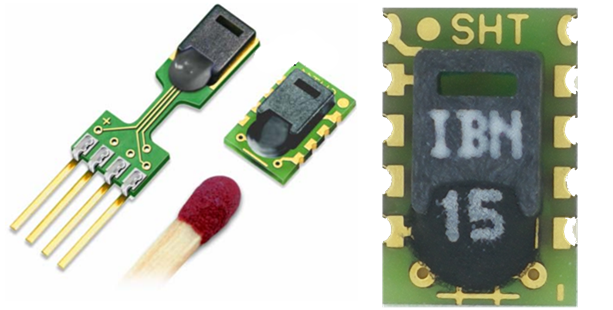
\includegraphics[width=0.3\textwidth]{06SHT15.png}
  			\bicaption[fig:SHT15]{SHT15温湿度传感器}{SHT15温湿度传感器}{Fig}{SHT15 humidity and temperature sensor}
		\end{figure}
		本系统选用SHT15温湿度一体传感器,如图\ref{fig:SHT15}所示,集成了温度测量元件、湿度测量元件和ADC,通过串口电路直接输出已校准的数字信号,响应快、可以较好的屏蔽干扰。且其采用2.4~5.5V宽电压供电,可以适应不同的供电要求,休眠时电流低至0.3 ,测量电流仅为550 ,具有良好的低功耗性能,符合温室环境监测低功耗的设计需求。该传感器在室温下测量精度可达到±0.3 ℃和±2\%RH,分辨率8~12 bits可调,量程-40 ℃~123.8 ℃和0~100\%RH,且长期稳定性好,符合温室内空气温度和湿度的测量要求
		
		(b) 土壤温湿度传感器
		
		一般情况下,温室内土壤温湿度分布均匀且变化缓慢,温室环境监测对于土壤温湿度的精度、灵敏度和测量范围要求不高,但是要求有较好的稳定性和线性,同时要可以适应各种复杂的土壤环境。
		
  		\begin{figure}[!htbp]
  			\centering
 			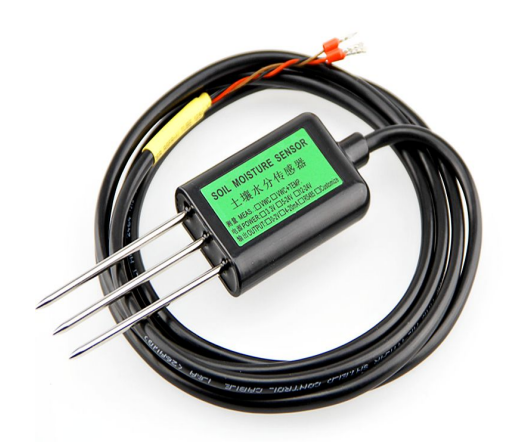
\includegraphics[width=0.3\textwidth]{07SMS50.png}
  			\bicaption[fig:SMS50]{SMS-II-50土壤温湿度传感器}{SMS-II-50土壤温湿度传感器}{Fig}{SMS-II-50 soil moisture and temperature sensor}
		\end{figure}
		本系统选用SMS-II-50土壤水分温度传感器,如图\ref{fig:SMS50}所示,集成了一个MS10土壤湿度传感器和一个热电阻温度传感器,包含电源稳压器和防反接电路,采用环氧树脂外壳,可以达到IP68级防护,可直接插入或埋入土壤中,具有良好的抗氧化和耐腐蚀能力,符合温室中恶劣环境的使用需求。具体性能参数如表\ref{tab:SMS50}所示。
			
		\begin{table}[!htbp]
  			\centering
  			\bicaption[tab:SMS50]{SMS-II-50性能参数表}{SMS-II-50性能参数表}{Table}{The performance parameters of SMS-II-50}
  			\begin{tabular}{lcc} \toprule
    		参数 & 土壤湿度 & 土壤温度 \\ \midrule
    		输出方式 & \multicolumn{2}{c}{0~2V模拟量/485输出} \\
    		测量量程 & 0-100\%(体积含水量) & -40-80℃\\
			测量精度 & ±5\% & ±0.5℃\\
    		响应时间 & \multicolumn{2}{c}{<1s} \\
    		供电电压 & \multicolumn{2}{c}{3.0-3.6V} \\
    		最大功耗 & \multicolumn{2}{c}{40mA} \\
    		土壤水分监测区域 & \multicolumn{2}{c}{以探针为中心,直径7cm,高度7cm的圆柱形区域} \\
    		防护等级 & \multicolumn{2}{c}{IP68} \\
    		探针和密封材料 & \multicolumn{2}{c}{探针:食用级不锈钢;密封:黑色阻燃环氧树脂} \\
    		安装方式 & \multicolumn{2}{c}{探针全部插入或整体埋入被测介质中} \\ \bottomrule
 			\end{tabular}
		\end{table}
		(c) 光照强度传感器
		
温室中的光照主要来自于太阳辐射和人工光照,光照强度测量范围主要为可见光波段。本文选用BH1750FVI光照强度传感器,具备I2C接口可以输出数字信号,采用高精度宽频谱的光电二极管,内置16bit ADC,在1-65535 lx的量程范围内具有平均分辨率1 lx,2.4~3.6V宽电压供电,成本和功耗低,可自动过滤50Hz/60Hz光噪声干扰,抗干扰能力强,适用于温室环境监测中应用。

		\subsubsection{底板模块}
		底板主要包括电源管理模块和接口模块。电源管理模块包含太阳能电池板与内置电池充电放电管理模块,以及传感器供电管理模块,通过收集温室环境能源即太阳能并储存于内置电池实现传感器系统的长期无值守工作。对外接口包括RS485接口、核心板接口和传感器接口。	
		
		\subsubsection{室外微型气象站和太阳辐射传感器}
		智能温室系统不仅需要对温室内的环境进行监测,还需要对室外的环境进行监测,两者结合才能更好地分析温室环境变化,更有效地对温室内环境进行控制。
		
  		\begin{figure}[!htbp]
  			\centering
 			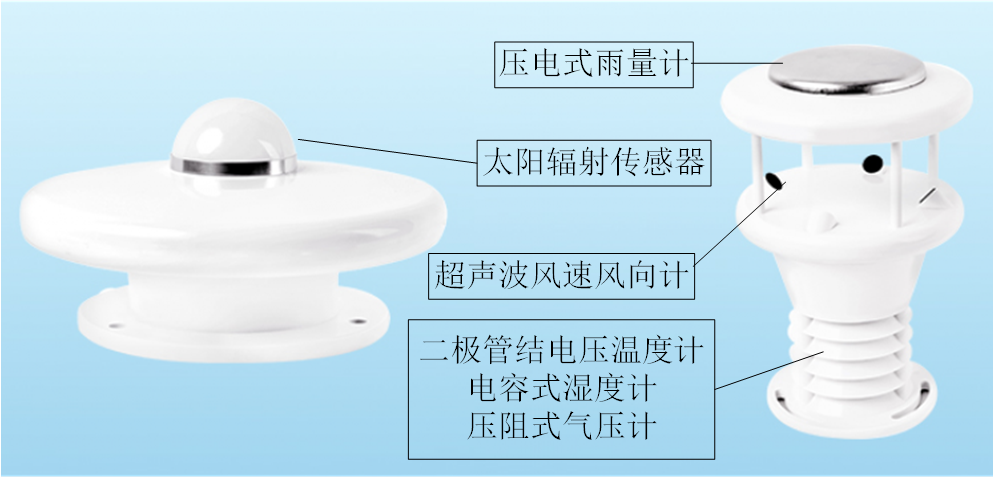
\includegraphics[width=0.6\textwidth]{08WeatherStation.png}
  			\bicaption[fig:WeatherStation]{MULTI-6P六要素微型气象站和GZ-300太阳辐射传感器}{MULTI-6P六要素微型气象站和GZ-300太阳辐射传感器}{Fig}{MULTI-6P 6-elements miniature weather station and GZ-300 solar light intensity meter}
		\end{figure}
		本系统选用智翔宇仪器MULTI-6P 六参数微型气象站和GZ-300 太阳辐射传感器,结构外观如图\ref{fig:WeatherStation}所示,可同时测量七种参数,如表\ref{tab:WeatherStation}所示\supercite{SunYuguang2009}。其中微型气象站包括采用超声波风速传感器、风向传感器,压阻式大气压传感器,二极管结电压空气温度传感器,电容式空气湿度传感器,压电式雨量传感器;太阳辐射传感器利用光电效应对太阳辐射强度进行测量;详细参数见表\ref{tab:WeatherStation}。微型气象站和太阳辐射传感器都采用一体化设计的金属外壳,抗污染和耐腐蚀性能强,采用紧凑和轻量化结构设计,易于安装拆卸,不需要现场维护和校准,可适应不同的工作环境。两者均采用12-30 V直流电源供电,可同时提供数字和模拟两种信号,其中数字信号输出为RS-485总线输出,供电和信号输入输出均通过底部航空插头,防护等级达到IP65级。
		
		\begin{table}[!htbp]
  			\centering
  			\bicaption[tab:WeatherStation]{MULTI-6P和GZ-300参数}{MULTI-6P和GZ-300参数}{Table}{The performance parameters of the MULTI-6P and GZ-300}
  			\begin{tabular}{ccccc} \toprule
			测量参数 & 测量原理 & 测量范围 & 测量精度 & 分辨率\\ \midrule
			空气温度 & 二极管结电压法 & -40-80 ℃ &	±0.5 ℃ &	0.1 ℃\\
			空气湿度 & 电容式 & 0-100\%RH & ±2\%RH & 0.1\%RH\\
			风速 & 超声波时差法 & 0-60 m/s & ±0.2 m/s & 0.1 m/s\\
			风向 & 超声波时差法 & 0-359.9° & ±3° & 0.1°\\
			大气压 & 压阻式 & 10-1100 hPa	 & ±0.5	 & 0.1 hPa\\
			雨量 & 压电式 & 0-200 mm/h	 & 	0.1 mm/h\\
			太阳辐射 & 光电效应 & 0-2000 W/$\text{m}^{2}$& ≤3\% & 	1 W/$\text{m}^{2}$\\ \bottomrule
 			\end{tabular}
		\end{table}

	\subsection{ZigBee网络定义}
	ZigBee无线网络中的设备按其功能分为三种,即协调器、路由器和终端节点。协调器是整个无线网络的通讯中心,主要用来组建网络、维护并管理路由器和终端节点入网等行为;路由器负责数据路由和路径选择,可以通过它方便的扩展网络覆盖范围;终端节点主要负责具体的信息采集任务\supercite{FuLingfeng2016} 。终端节点和路由器通过无线信道向协调器上报传感数据,协调器再把接收的数据通过RS485总线上传至上层系统。
	
本系统的底层ZigBee无线传感器网络基于Z-Stack协议栈开发,开发人员可以直接调用协议栈提供的API来实现相应的功能而无需深入了解完整的ZigBee协议等,可以极大程度上为开发工作提供便利,减少开发时间。

	\begin{figure}[!htbp]
		\centering
	    \subfigure[协调器]{
			\label{fig:zigbee:a} 
			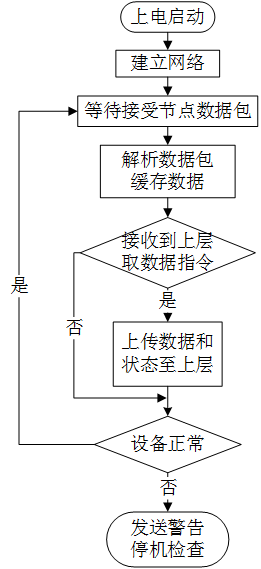
\includegraphics[width=0.25\textwidth]{zigbee/2.png}
		}
	    \subfigure[路由器]{
			\label{fig:zigbee:b} 
			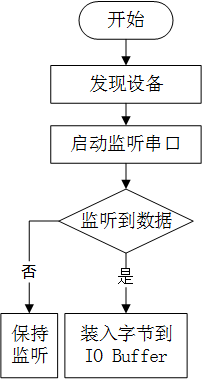
\includegraphics[width=0.25\textwidth]{zigbee/1.png}
		}
		\subfigure[终端节点]{
			\label{fig:zigbee:c}
			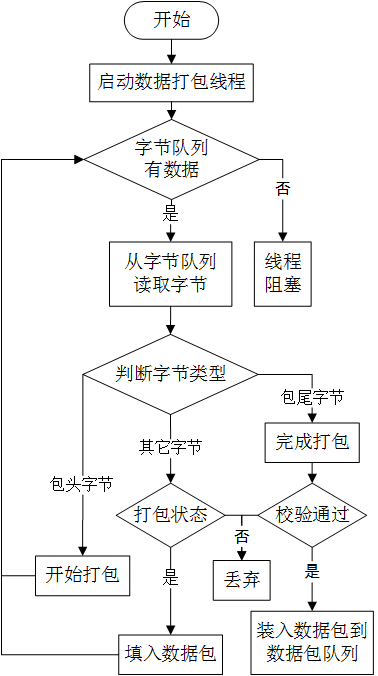
\includegraphics[width=0.25\textwidth]{zigbee/3.png}
		}
	    \bicaption[fig:zigbee]{自定义ZigBee通信流程}{自定义ZigBee通信流程}{Fig}{Self-defined ZigBee communication flow}
	\end{figure}
在ZigBee网络中,协调器对于整个网络的组建、维护和管理,以及路由器的数据路由功能均由协议栈的功能函数实现的。通过在协议栈基础上制定自定义通信协议和流程,实现项目需要的协调器的广播指令、数据解析、数据缓存、与上层设备的串口通讯、终端节点的数据采集、低功耗休眠和唤醒、数据解析和打包、电池状态监测上传等功能。自定义ZigBee通信流程如图\ref{fig:zigbee}所示。

协调器建立网络后,随时等待处理路由器和终端节点的加入,并随时等待已加入网络的路由器和终端节点上传数据;当接收到上传的数据包时将执行数据包解析并将解析到的数据缓存到本地,同时通知上层程序获取数据;当接收到上层程序获取数据指令时,将缓存的数据上传至上层程序。

终端节点上电加入网络后,首先会向上层发送一条检测数据以及时告知节点变化,随后定时休眠,唤醒后自动打开传感器供电,开始采集环境参数,同时检查传感器状态和电池电量,随后节点关闭传感器供电,将数据和状态信息封装后上传至上层节点,然后定时休眠进入下一个循环。为避免终端节点同时向协调器上传数据所带来的信道拥挤和数据包丢失的问题,本系统的自定义ZigBee通信流程未采用统一休眠唤醒并采集上传数据的方式,而是采用节点自主休眠唤醒、执行采集动作并上传的方式,有效地解决了大量节点同时上传数据时信道冲突的问题。路由器具有和终端节点相同的数据采集功能和类似的通信流程,只是不执行定时休眠唤醒,而只执行定时采样。

此外,协调器还可以向网络中的任意一组或全部设备发送广播命令,如统一修改休眠时间、统一修改采样周期等。

通信流程定义了ZigBee网络中的数据传输方向和顺序,为方便与上层程序通信,还需要定义数据包的格式。该网络中将数据包分为指令包、响应包和采集包。

指令包为上层程序向协调器发送的命令数据,可以设置休眠时间、获取缓存数据等。数据包长度共9 byte,分别为起始符、长度位、功能码、数据段、校验码和终止符,除数据段为4 byte外其余均为1 byte。起始符和终止符为0x3A和0x23,功能码0x01表示重置参数,0x02表示请求数据,0x03表示设置休眠时间,0x04表示设置采样周期,设置休眠时间和采样周期时数据段内为需要设置的时间,其余情况数据段均为0,校验码为求和校验的校验码。

响应包为向上层数据反馈的数据,共5 byte,分别为起始符、长度位、功能码、校验码和终止符,均为1 byte。起始符和终止符为0x25和0x26,功能码0x01表示重置参数成功,0x02为有数据缓存完成,0x03为设置休眠时间成功,0x04为设置采样周期成功。

采集包为传感器采集的数据包,详情如表\ref{tab:sampling}所示。网络地址为节点在网络中由协调器分配的地址;设备ID为自定义的设备编号;状态位为设备的状态信息,从bit7到bit4分别对应电池状态、空气传感器状态、土壤传感器状态、光强传感器状态,其余待定,0为正常,1为异常;数据长度为数据的长度;数据为具体的数据数值,每5 byte表示一个参数的数值,以ASCII码传输和保存。

		\begin{table}[!htbp]
  			\centering
  			\bicaption[tab:sampling]{采集包格式}{采集包格式}{Table}{The format of sampling package}
  			\begin{tabular}{cccc} \toprule
			单元 & 	字节数 & 	描述 & 	缩写\\ \midrule
			包头 & 	1 & 	3A(:)	 & SD\\
			网络地址 & 	2 & 	 & 	ADDR\\
			设备编号 & 	2 & 	 & 	ID\\
			状态码	 & 1	 & &  	ST\\
			数据长度	 & 1	 &  & 	LEN\\
			数据 & 	n & 	ASCII码 & 	DATA\\
			校验码	& 1	 &  & 	XOR\\
			包尾	& 1	 & 23(\#) & 	ED\\ \bottomrule
 			\end{tabular}
		\end{table}
		
	\subsection{低功耗优化}
	节点功耗主要产生在核心板的运行和传感器的工作上。由于智能温室的数据实时性要求不高、采样和上传周期长,所以低功耗优化主要从缩短节点工作时间和传感器采集供电时序优化两方面进行。
	
节点功耗测试结果表明,休眠期间的平均电流仅为其工作期间的1/50左右。因此,在一个数据上传周期里,可使节点在绝大部分时间处于休眠模式,定时唤醒后立即采集数据并上传,完成后立即进入休眠模式,依次循环。

此外可根据数据变化的实际情况和理论规律配置不同的采样周期。结合传感器的响应特性,对传感器采用分时供电策略。在节点唤醒后,对响应速度快的MS10和BH1750FVI供电预热1.2 s后采样,对响应速度慢的SHT15预热5 s后采样。

测试结果显示,相比于一直处于工作状态的无低功耗优化的节点,低功耗优化后每10分钟唤醒工作的节点功耗大幅度减少96.3\%,与太阳能电池板配合工作,可以满足温室传感器长期无值守的工作要求。

	\subsection{控制模块}
	感知控制层除了对温室环境进行监测之外,还需要对温室环境进行控制,主要通过控制温室内的作动器来实现。温室内作动器控制主要通过中央控制板完成,如图\ref{fig:ControlBoard}所示为中央控制板及其功能框图,包括微控制器、RS485通讯接口、设备状态控制显示模块和电源管理模块。微控制器选用片上资源丰富STM32F103系列单片机,使用它的UART连接RS485模块完成与上层系统的通讯。设备控制利用继电器组实现。为保证设备的准确控制,控制板通过开关状态模块采集设备当前状态。控制板将当前设备状态与预设控制状态比对来分析现场设备或控制板的故障情况然后上报,以便系统能及时发现问题,满足本系统的自诊断需求。
	
	\begin{figure}[!htbp]
		\centering
		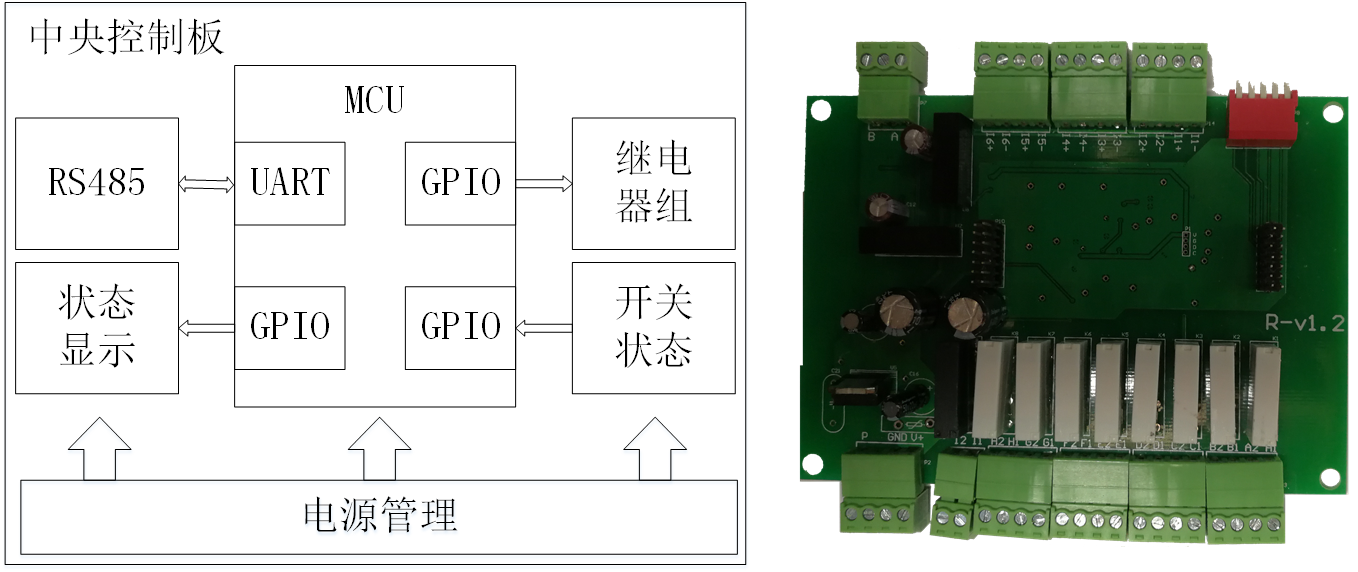
\includegraphics[width=0.7\textwidth]{09ControlBoard.png}
		\bicaption[fig:ControlBoard]{中央控制板及其功能框图}{中央控制板及其功能框图}{Fig}{The photo and function diagram of the central control board}
	\end{figure}
	\subsection{图像采集模块}
图像采集部分采用HIKVISION CSC4S51WEFR网络摄像头,如图\ref{fig:Camera}所示,接入图像采集网关可直接在局域网内对温室进行视频监控,如果温室现场网络条件良好,可接入云端服务生成m3u8视频流,提供在线视频观看,对于部分温室现场网络条件欠佳,本系统将通过定时采集现场静态图片的方式提供图像,同时接入云端图片存储服务,并返回对应URL。

	\begin{figure}[!htbp]
		\centering
		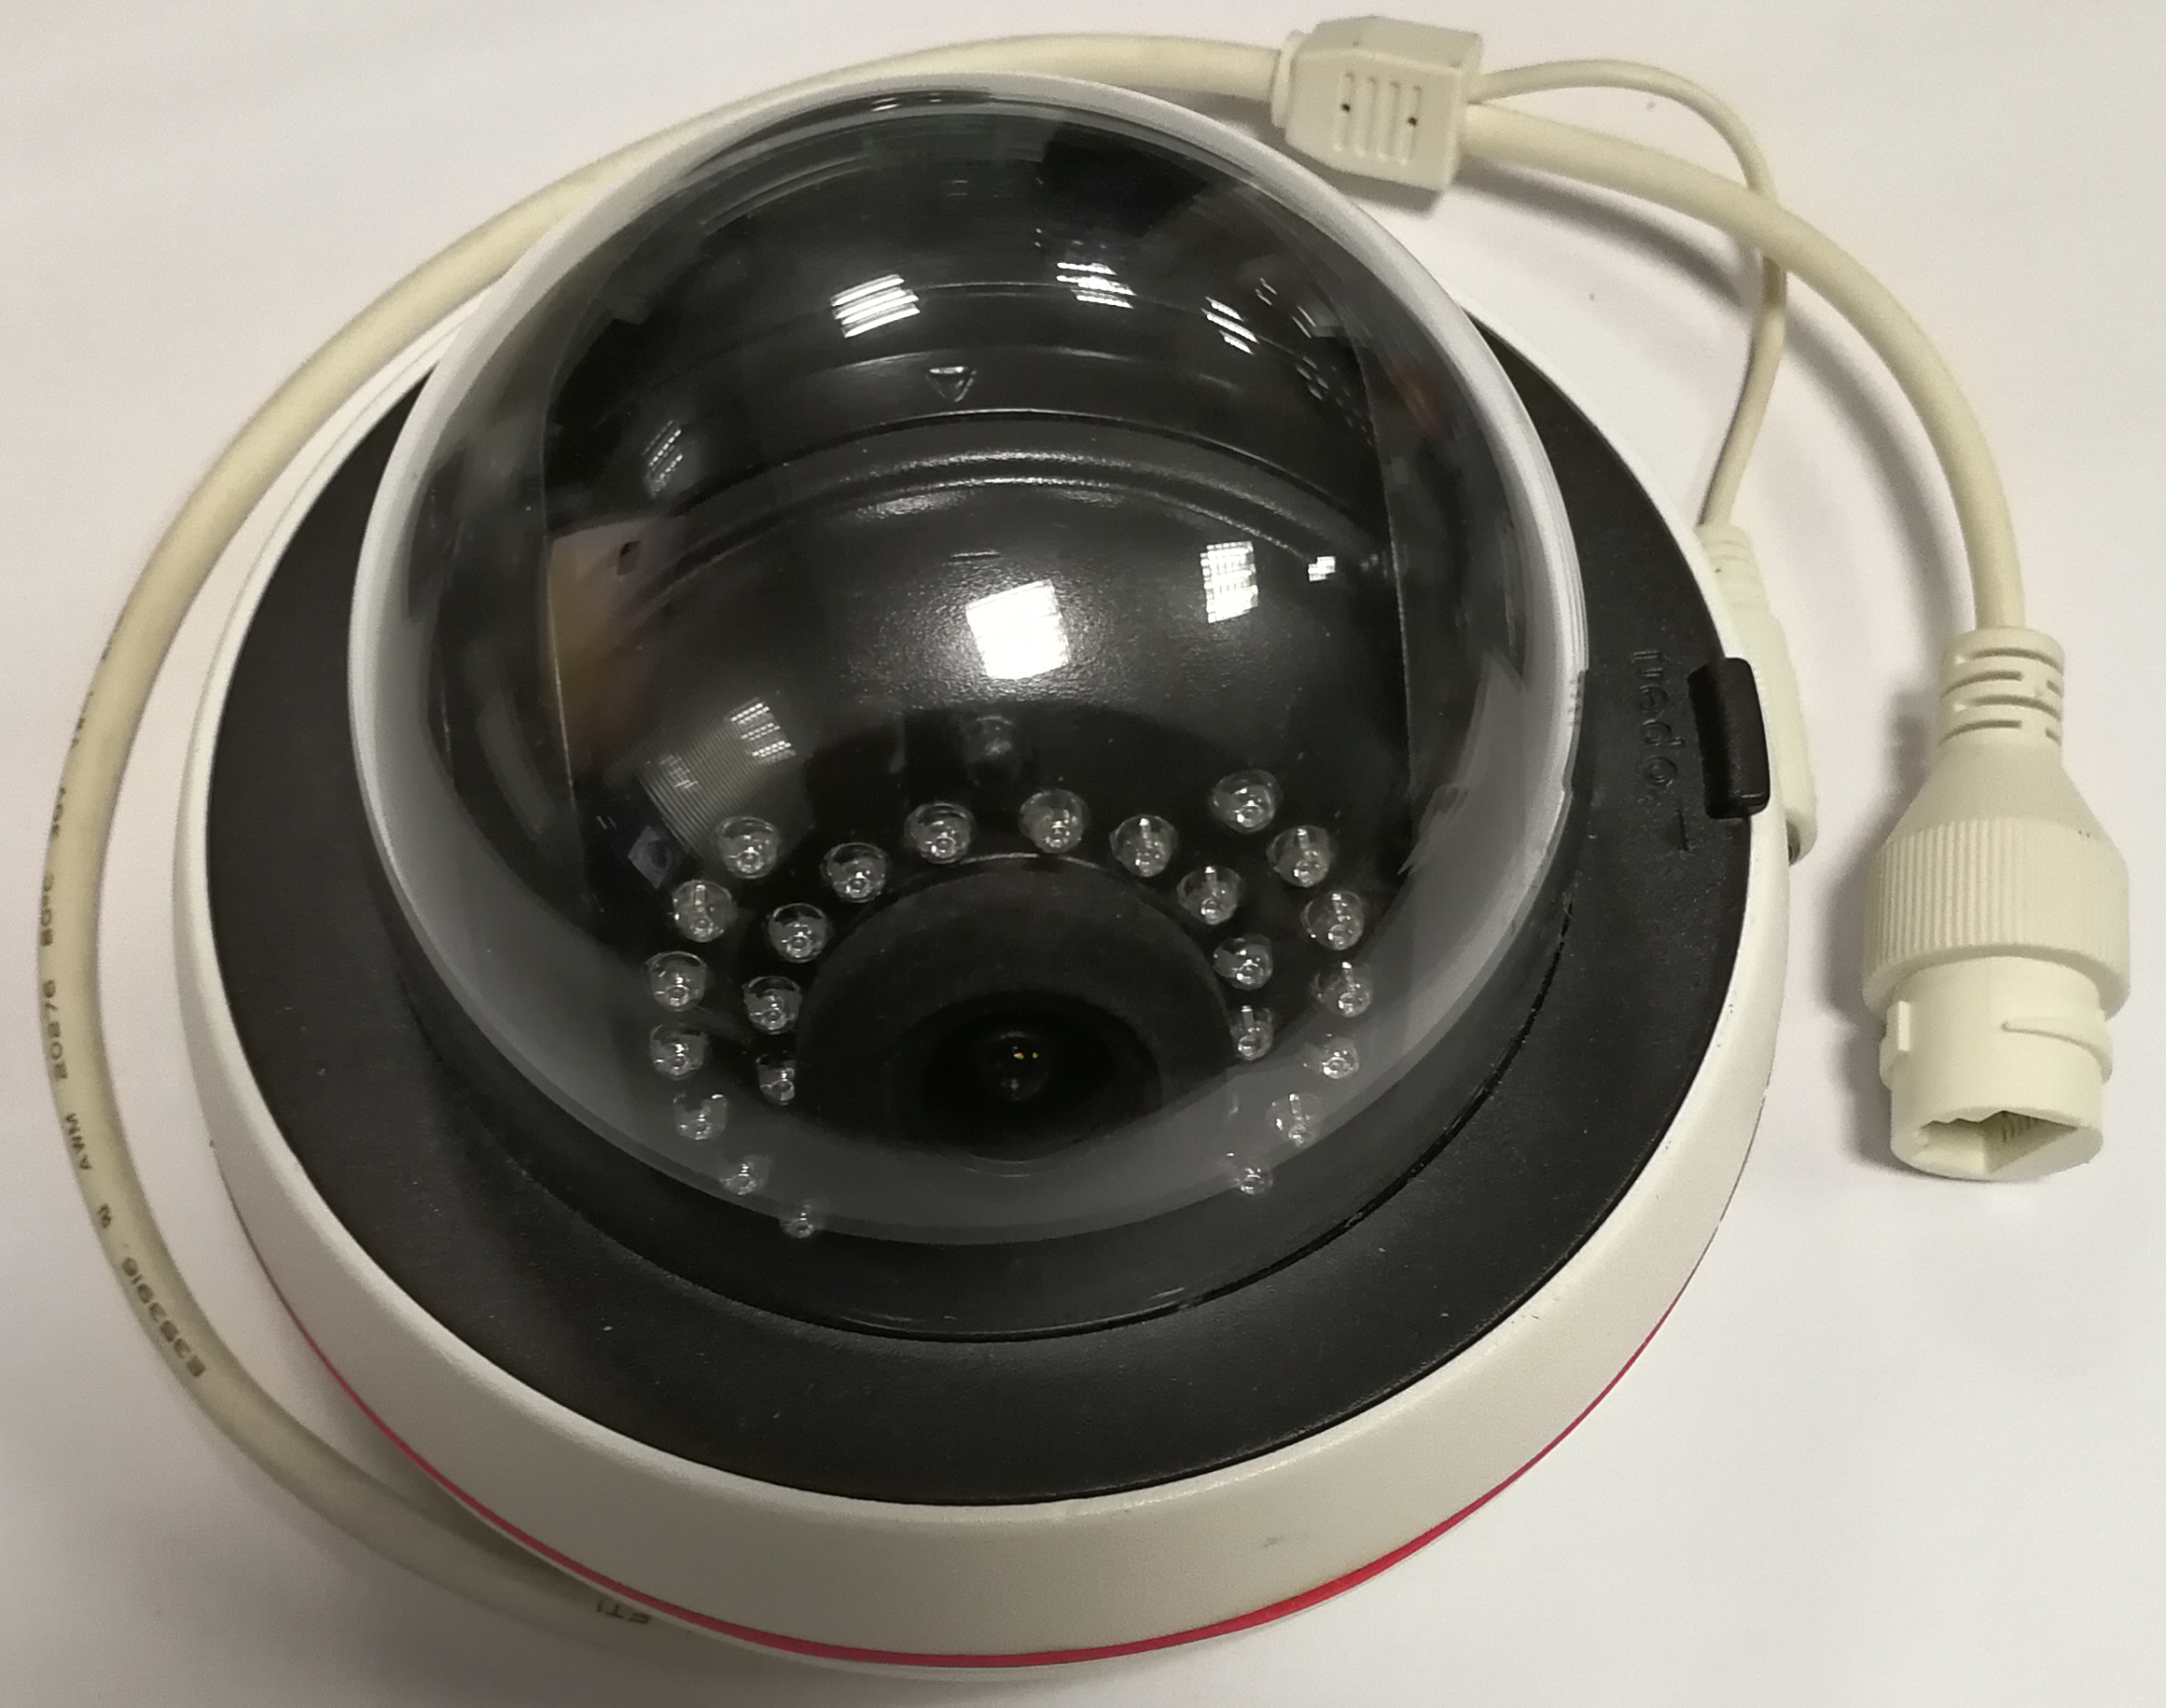
\includegraphics[width=0.3\textwidth]{10Camera.png}
		\bicaption[fig:Camera]{HIKVISION CSC4S51WEFR网络摄像头}{HIKVISION CSC4S51WEFR网络摄像头}{Fig}{HIKVISION CSC4S51WEFR web camera}
	\end{figure}
\section{网络传输层设计与实现}
	\subsection{总体设计及技术简介}
	本文智能温室中的网络传输层通过数据传输与同步系统实现,该系统可实现控制指令和反馈信息的双向传输,以及传感器监测数据的上传与同步。其中监测数据的同步模块大部分部署在云端服务器,另一部分以及其余模块均部署运行在搭载Linux操作系统的基于ARM Cortex-A53的微型计算机上,该计算机具有64位4核CPU,主频为1.2 GHz,1 GB LPDDR2内存,最大支持64 GB内存卡,同时支持以太网连接和Wi-Fi连接,自带蓝牙4.1模块,4个USB接口,40个GPIO引脚,完全可满足现场计算服务的性能和通讯需求。
	
本系统内所有程序均采用Java语言编写,为进行串口通讯引入RXTX,使用Spring进行依赖注入管理和AOP编程 ,选择MyBatis作为数据持久化框架 ,数据库采用MySQL,未来将考虑使用更加轻量级、更加适用于嵌入式系统的SQLite代替MySQL作为现场数据存储数据库。

Java是一种功能强大且简单易用的面向对象编程语言,开源社区活跃,拥有众多优秀的开源框架和类库,可以快速便捷地开发各种跨平台的应用程序\supercite{ThinkingInJava}。RXTX是一个可开源Java串口库,具有良好的跨平台性,且向下兼容javax.comm串口库。Spring是一个轻量级的依赖注入管理和面向切面编程的容器框架,可以简化企业级Java应用的开发,极大地提高开发者的开发效率\supercite{spring}。MyBatis是一款开源的优秀持久层框架,使用简单的注解或配置,即可将通过接口将Java中的POJOs映射成数据库中的记录\supercite{mybatis}。MySQL是一款开源的非常轻量级的关系型数据库管理系统,功能强大,性能良好,且具有较小的体积,在世界范围内得到广泛的应用。

	\subsection{控制信息解析传输}
系统中的控制指令和反馈信息的双向传输,通过控制信息解析传输程序实现,该程序部署在Tomcat容器中。
	
该程序的工作流程如图\ref{fig:control}所示。

	\begin{figure}[!htbp]
		\centering
		\includegraphics[width=0.8\textwidth]{control.png}
		\bicaption[fig:control]{控制信息解析传输程序流程图}{控制信息解析传输程序流程图}{Fig}{Flow chart of control information transmission}
	\end{figure}
程序向外暴露RESTful WebService接口,为了保证系统控制的安全性,避免恶意操作和非法操作等,系统会对所有请求的来源和合法性进行判断,所有接口仅向云端服务器开放,即如果该请求不是来自于指定的云端服务器,或者请求是非法的,均会被视为无效请求,将被立即拒绝并返回相应的错误信息。随后系统会对请求进行身份和权限鉴定,以避免误操作可能对温室设备带来的损坏,如果请求发起者没有相关操作的权限,请求将会被拒绝并返回相应的错误信息。随后系统根据不同的请求类型分别执行相应的动作,若操作成功则返回成功响应,否则返回响应的错误信息并向管理员发送告警通知。

	\subsection{数据采集上传}
	传感器网络的数据监测和同步上传,通过数据采集上传程序实现,程序的具体工作流程如图\ref{fig:thread}所示。
	
	\begin{figure}[!htbp]
		\centering
		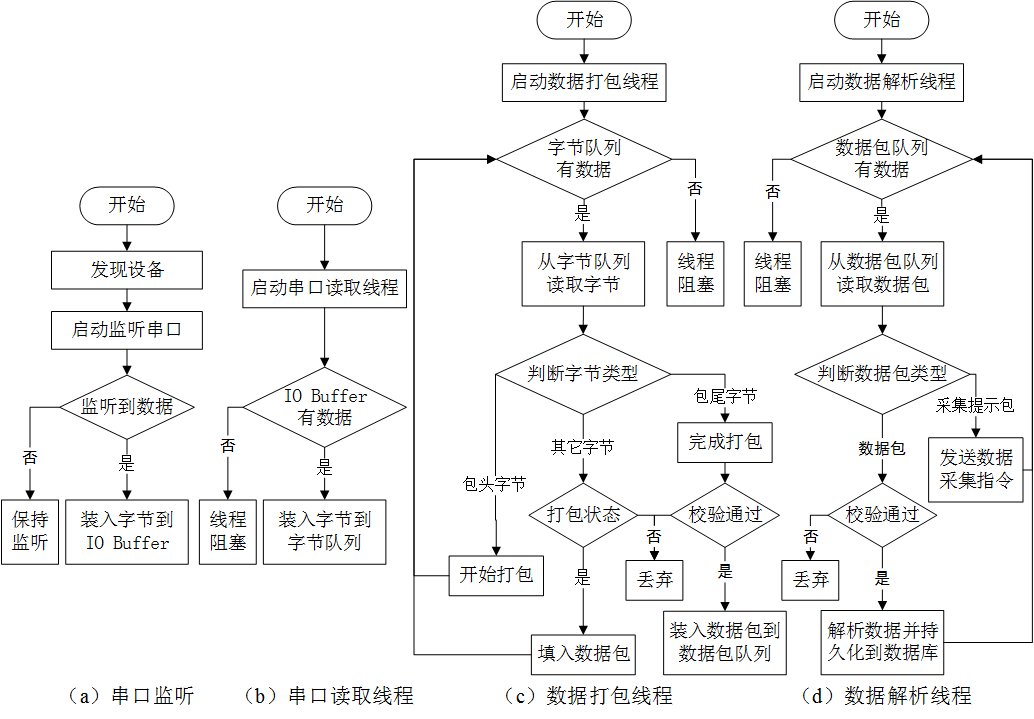
\includegraphics[width=1\textwidth]{thread/thread.png}
		\bicaption[fig:thread]{数据采集上传程序流程图}{数据采集上传程序流程图}{Fig}{Flow chart of data sampling and uploading}
	\end{figure}
首先程序将会去发现可用的串口设备,随后打开串口监听并保持,当监听到有效数据时将字节装入IO Buffer,如图\ref{fig:thread}(a)所示。

然后为了解决由于串口数据上传不完整而导致的数据包丢失问题,程序将同时启动如下四个线程,并采用生产者消费者的设计模式:
	\begin{enumerate}
		\item 串口读取线程。当串口IO Buffer中有缓存数据时,线程将从IO Buffer中读取字节流,并填入字节队列中,当IO Buffer无数据为空时,线程将阻塞等待。详细流程如图\ref{fig:thread}(b)所示。
		\item 数据打包线程。当字节队列中有数据时,线程从字节队列中读取字节并判断字节的类型:当读到包头字节即起始符时进入打包状态;当读到包尾字节即终止符时完成打包并对数据包进行校验,校验通过后装入数据包队列,否则丢弃并恢复普通状态;当读到其它字节时如果处于打包状态则将字节装入数据包,否则丢弃该字节。字节队列使用无限阻塞队列,意味着当字节队列为空时,线程继续从队列中获取对象将阻塞等待;如果队列中还存在未处理完成的字节时,读入的字节将添加在队列尾部。详细流程如图\ref{fig:thread}(c)所示。
		\item 数据包解析线程,当数据包队列中有数据包时,线程将从数据包队列中读取数据包并判断数据包的类型:当读到采集提示包时将向下层协调器发送数据采集指令;当读到数据包时则对数据包进行校验,校验通过后解析数据包并持久化到数据库,否则丢弃。数据包队列同样使用无限阻塞队列,数据包队列为空时,线程将阻塞等待。详细流程如图\ref{fig:thread}(d)所示。
		\item 采集指令发送线程,该线程会定时向室外气象站和太阳辐射强度传感器发送数据采集指令。
	\end{enumerate}
	
	\subsection{数据同步}
到目前为止所有的监测数据还都存储在温室群本地的现场微型计算机上,但是该现场微型计算机性能和存储空间有限,同时由于农业生产环境的限制,温室群所在地区网络环境一般较差,这给温室数据的远程获取带来了一定的阻碍,有可能会出现数据获取缓慢,甚至无法获取的情况,因此,本系统将所有监测数据同步到云端数据中心的数据库中,所有应用对于数据的获取将全部从云端数据库获取,这就解决了上述问题。

	\begin{figure}[!htbp]
		\centering
		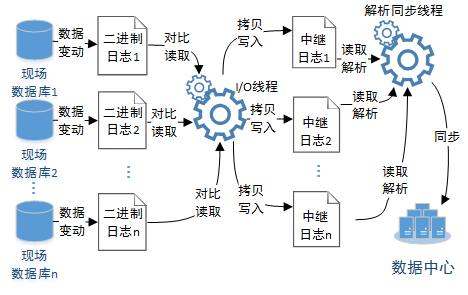
\includegraphics[width=0.6\textwidth]{11Sync.png}
		\bicaption[fig:Sync]{数据同步过程}{数据同步过程}{Fig}{Process of the data synchronization}
	\end{figure}
监测数据的同步通过数据同步程序实现,如图\ref{fig:Sync}所示,现场数据库在每个事务更新数据完成之前,会将这些事务串行地写入二进制日志中去,在事件日志写入完成之后将发出通知。随后云端同步程序将建立一个I/O线程对现场数据库的二进制日志文件进行订阅,当收到数据变动通知时将与现场数据库建立连接,随后将开始Binlog dump process从日志中读取相关事件,完成后将睡眠并等待通知,同时将事件写入中继日志,随后解析同步线程将提取中继日志中的事件进行解析并尝试向云端同步。

\section{应用及终端接入层设计与实现}
	本系统的数据中心和WEB服务器均部署和运行在云端服务器,具有高安全、高可用、灵活扩展、成本低等特点。
	\subsection{数据中心}
本系统的数据中心基于Hadoop构建,其中海量实时数据库使用HBase,数据仓库使用Hive,并使用MySQL作为近期历史数据的存储数据库。

Hadoop是一个分布式系统基础架构,可以对海量数据进行分布式的存储和处理,稳定可靠、易于扩展、性能突出、高度容错且成本低廉,是存储海量温室数据的较好的选择\supercite{hadoop} 。HBase是一个面向列的NoSQL数据库,为了解决HDFS难以随机读写和缺乏实时性而出现\supercite{hbase} 。Hive是一个数据仓库工具,可以将SQL语句转换为MapReduce任务,极大程度地减少了开发人员的MapReduce jobs的编写工作\supercite{hive} 。

	\begin{figure}[!htbp]
		\centering
		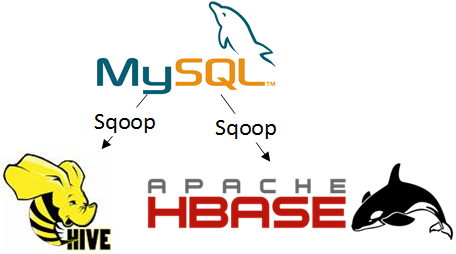
\includegraphics[width=0.5\textwidth]{12Data.png}
		\bicaption[fig:Data]{ MySQL与Hive、HBase之间的迁移关系}{ MySQL与Hive、HBase之间的迁移关系}{Fig}{The relationship among MySQL and Hive/HBase}
	\end{figure}
数据中心通过MySQL接收下层系统同步上传的数据,以一个温室群布置30个终端节点和路由器节点,每10 min采集一组数据为例,仅传感监测数据每天可产生2.2×104条记录,每年可产生 8×106条记录,室外气象参数监测每天也将产生大量的数据,同时温室控制每天还将产生大量控制日志记录,这样一个温室群每年将产生数千万条数据,多个温室群每年将产生数亿条数据,这会严重影响MySQL工作效率,虽然进行分库分表操作可一定程度上缓解这种问题,但是将增加数据库复杂度,而且考虑到在实际生产中,经常访问的均为近期的监测数据,大量历史数据仅需用于后期的查询、导出和分析。因此,本系统定期地将把MySQL中历史数据通过Sqoop工具\supercite{sqoop} 迁移至HBase和Hive中保存,迁移关系如图\ref{fig:Data}所示,MySQL数据库中仅保存温室近期数据。HBase和Hive中的历史数据将用于后期数据分析和控制策略的机器学习。
 
	\subsection{WEB服务器}
温室环境监测数据采集完成并同步到云端的数据中心,系统还需要向外界提供相关的服务,包括提供温室环境远程监测查看、温室环境远程控制、温室现场视频或图像查看等服务,因此需要WEB服务器及其相关服务端程序。

本系统选用商用云服务器作为WEB服务器,可提供7×24小时不间断服务保证,简单高效,处理能力和存储空间可弹性伸缩,免除了机房维护的问题,降低了运维成本。服务器上运行64位CentOS 6.5操作系统,CentOS是当今最流行的服务端Linux发行版之一,由Red Hat Enterprise Linux依照开放源代码规定公布出的源代码编译而成,具有高度的稳定性和可靠性、良好的性能,因此非常合适作为服务端操作系统。

	\begin{figure}[!htbp]
		\centering
		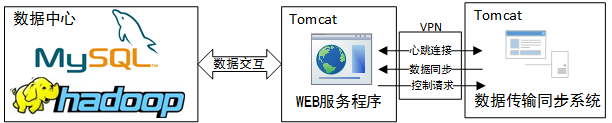
\includegraphics[width=0.8\textwidth]{13Web.png}
		\bicaption[fig:Web]{WEB服务程序工作流程}{WEB服务程序工作流程}{Fig}{Workflow of the webservice}
	\end{figure}
WEB服务端程序均部署在Tomcat容器中,全部使用Java语言编写,基于典型SSM框架开发,即Spring + Spring MVC + MyBatis框架,采用MVC(Model View Controller)分层设计模型,其中Spring为程序提供必要的依赖注入和AOP框架,Spring MVC作为程序的轻量级请求驱动的WEB应用框架,可以方便地实现MVC模型,MyBatis则为程序提供了数据持久层框架。
 
WEB服务程序工作流程如图\ref{fig:Web}所示。所有数据均与数据中心进行交互。考虑到安全因素,保证系统的安全性,服务器向下通过VPN(Virtual Private Network)连接数据传输与同步系统,可调用控制接口对温室设备进行控制,接收数据同步请求进行数据同步,同时建立心跳连接以确定与下层系统的网络连通状态,以便于及时通知系统管理人员当前系统的状态。同时向外暴露RESTful WebService接口,供终端程序调用并返回JSON格式数据,实现前后端分离设计,也可为其它接入的系统提供相关服务。

	\subsection{智能策略学习控制子系统}
智能温室监测与控制不仅要解决温室内环境远程监测与远程控制的问题,更进一步是要解决温室的智能控制,即温室在不需要人工参与的情况下可以实现自主根据当前的温室环境参数,控制温室各种可用作动器的单独动作或组合动作,完成温室环境的控制调节。

温室是一个流场、温度场、浓度场等多物理场耦合在一起的多输入多输出的大时延系统,对温室任何目标的控制,都会影响到其它状态的变化,且对于外界所施加的作用,温室都会经过一段延时后才会有所响应。这些因素都导致温室环境控制是一个极其复杂和困难的问题。为了解决温室控制的问题,本系统采用专家经验提供初始策略,CFD仿真模拟提供优化分析建议,机器学习模型持续训练迭代的方式。

传统的温室环境控制多依靠农业生产人员以及专家的经验来进行,但是中国幅员辽阔,地区差异极大,每个温室又各不相同,经验往往是有针对性的,难以适应不同温室的控制需求。针对以上这些问题,本系统设计了智能策略学习控制子系统,该子系统根据专家经验制定初始的控制策略,通过CFD仿真技术和机器学习技术,实现温室环境控制策略的优化,以及控制策略后期的自主学习,不断完善控制策略,改善控制效果。

借助CFD仿真技术可以更加清晰、定量化地了解温室的结构参数、作动器的不同动作组合、温室内外的环境参数对于温室环境参数变化和分布的影响。根据经过验证的温室CFD模型,系统可以得到任意环境条件下,任意温室内的任意作动器动作引起的温室环境的变化和分布,通过稳态和瞬态的分析,不仅可以了解控制效果,还可以了解其变化过程,这些都可以帮助更好地优化控制策略,改善控制效果,同时减少能源消耗。

机器学习技术可以让系统控制策略根据温室环境的历史数据、温室控制日志的历史数据和温室作动器的不同控制组合不断更新迭代已有的控制策略,实现温室控制策略的自主学习和自适应学习。系统可采用K-means算法对温室环境的历史数据进行聚类并按照规则打分,然后利用改进的Apriori聚类分析算法对控制日志历史数据、控制组合和已分类的温室环境历史数据进行聚类找出其中最有的组合并根据结果决定是否更新当前控制策略。

	\subsection{终端程序}
终端程序分为WEB页面程序和移动终端程序,均可接入智能温室系统的应用层,实现温室远程监测和控制,以及温室现场的图像与视频监控。

所有前端程序均部署在云端Nginx服务器,该服务器资源消耗小,并发能力强,稳定性高,有丰富的功能集,且高度可配置。

WEB页面使用HTML5 + CSS3 + JavaScript开发,使用Node.js作为JavaScript开发运行环境,主要使用的技术栈有React、Redux、Webpack和Sass,使用React Router作为前端路由器库,通过AJAX技术调用应用层所提供的接口,得到JSON数据,并将数据按照自定格式解析后展示到页面。

其中Node.js是一个基于Chrome V8 引擎的轻量高效的JavaScript 运行环境。React是Facebook开源的一款前端JavaScript MVC框架,主要解决View层的开发,官方给它的定义是一套用来生成用户界面的JavaScript库,为了配合React开发,前端选用React Router作为路由库,用以管理资源路径,实现组件的切换和状态的变化。为了确保前端页面状态的可预测性,使用Redux作为前端页面容器。Webpack 是目前非常流行的开发便捷、扩展性强的前端资源模块加载器和打包工具,利用Webpack可以按照依赖关系和相关规则将松散的模块打包成符合生产环境部署的前端资源,还可以将按需加载的模块进行代码分隔,等到实际需要的时候再异步加载,通过加载器的转换,不仅仅是JS,任何形式的前端资源都可以视作模块,比如ES6模块、CSS、图片、JSON等。Sass是一种成熟、稳定而且非常强大的专业级CSS扩展语言,完全兼容CSS语法,同时提供了许多便利的写法,大大节省了设计者的时间,使得CSS的开发,变得简单和易维护。AJAX即“Asynchronous JavaScript And XML(异步JavaScript和XML)”,是指一种用来创建交互式网页应用的网页开发技术,它使得页面可以异步更新,即只对其中的局部进行刷新而无需全部重新刷新。JSON(JavaScript Object Notation) 是一种数据交换格式,在让人可以非常容易读写的同时还非常便于机器的解析生成。

移动客户端使用React Native开发,React Native同样是Facebook开源的一套前端应用技术框架,开发者通过React Native可利用JS和React创建原生移动应用,并且可复用大部分代码同时生成Android平台和IOS平台应用。移动应用同样调用应用层提供的接口获得返回数据,然后经过解析展示到界面。

	\begin{figure}[!htbp]
		\centering
	    \subfigure[温室选择页]{
			\label{fig:ui:a} 
			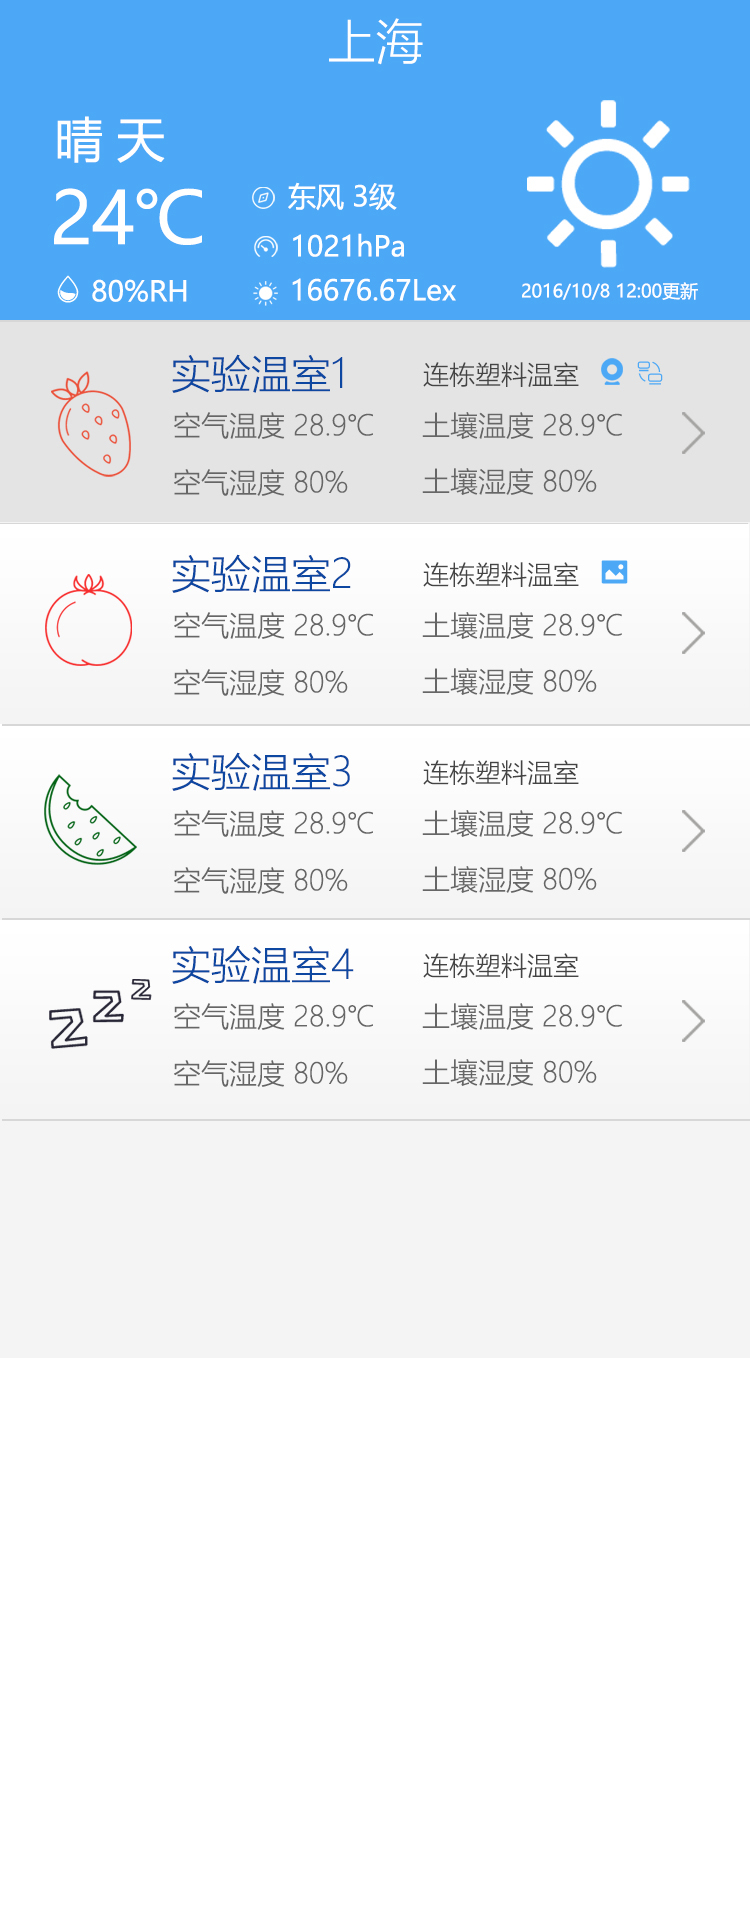
\includegraphics[width=0.18\textwidth]{UIDesign/home.jpg}
		}
	    \subfigure[温室详情页]{
			\label{fig:ui:b} 
			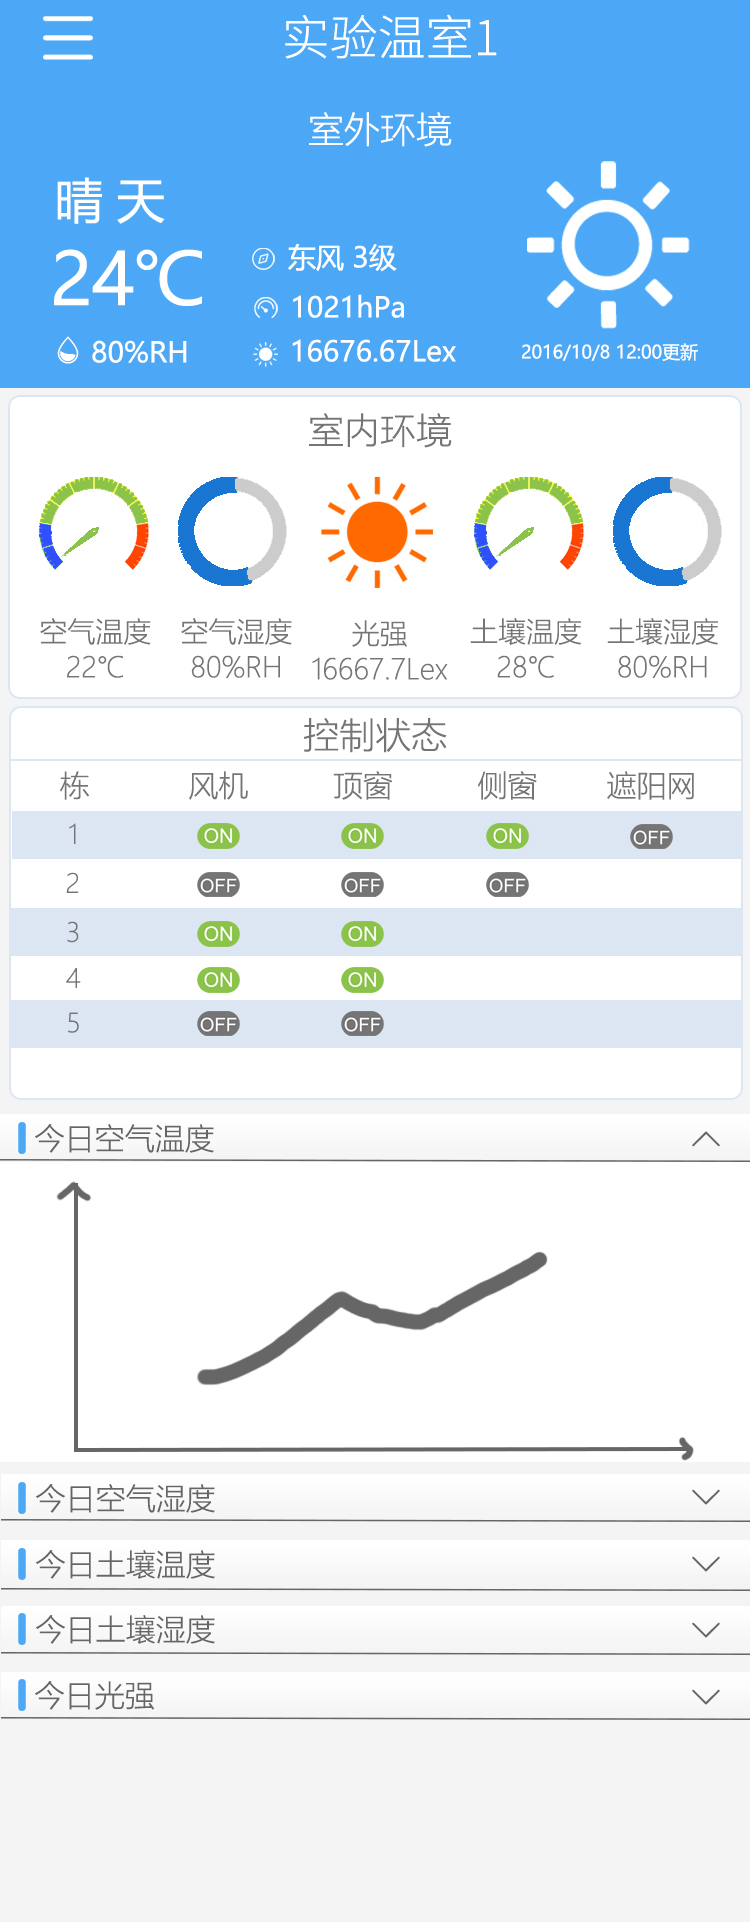
\includegraphics[width=0.18\textwidth]{UIDesign/detail.jpg}
		}
		\subfigure[历史曲线页]{
			\label{fig:ui:c}
			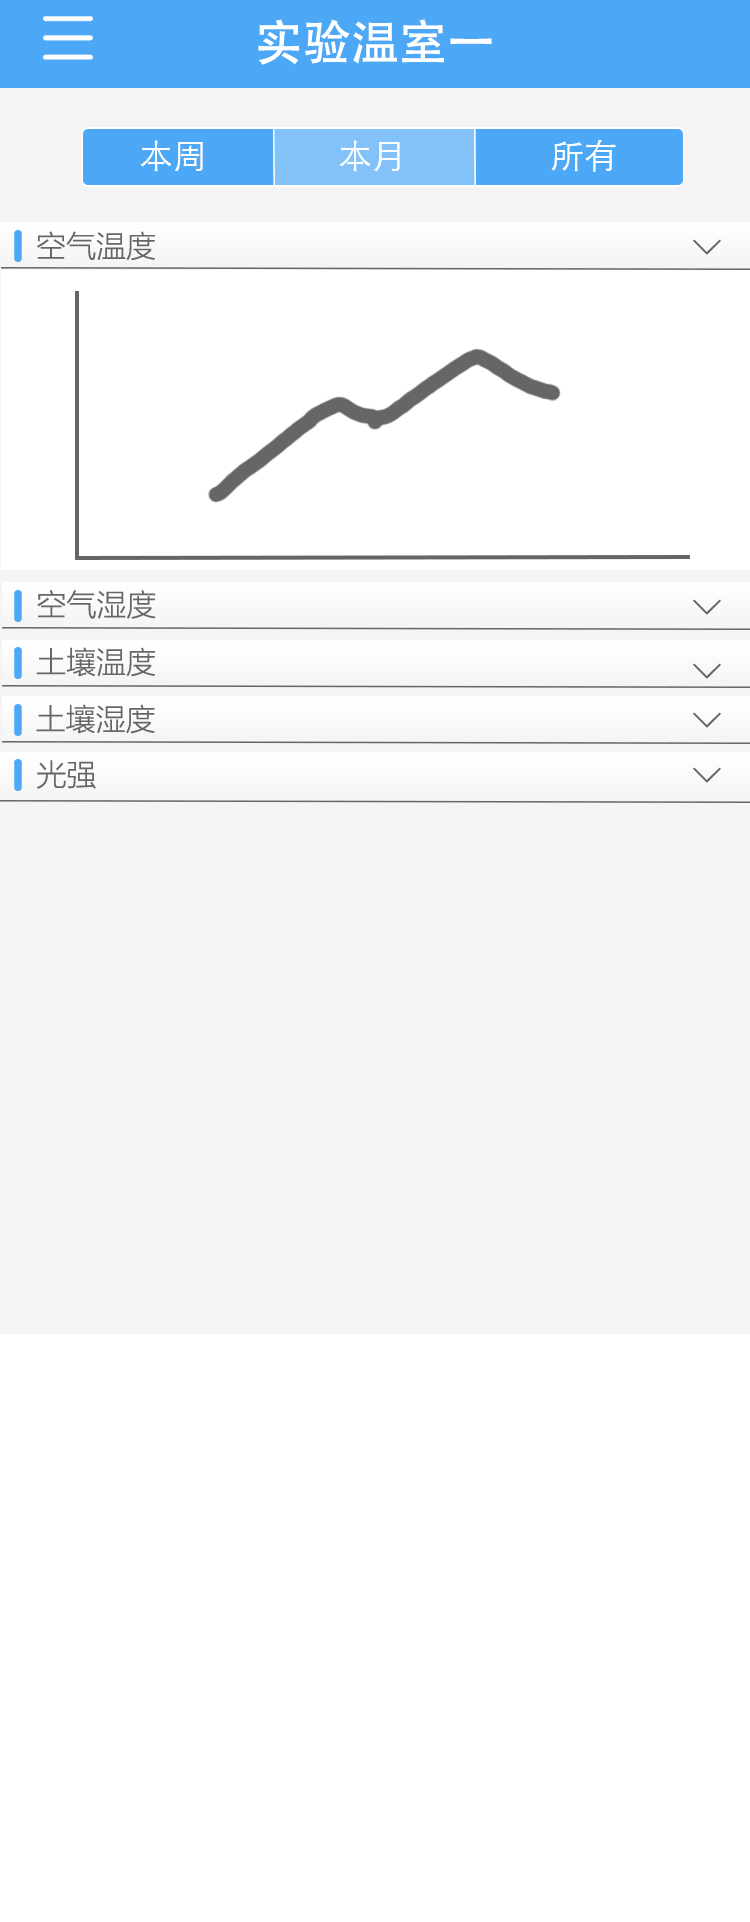
\includegraphics[width=0.18\textwidth]{UIDesign/history.jpg}
		}
		\subfigure[温室控制页]{
			\label{fig:ui:d}
			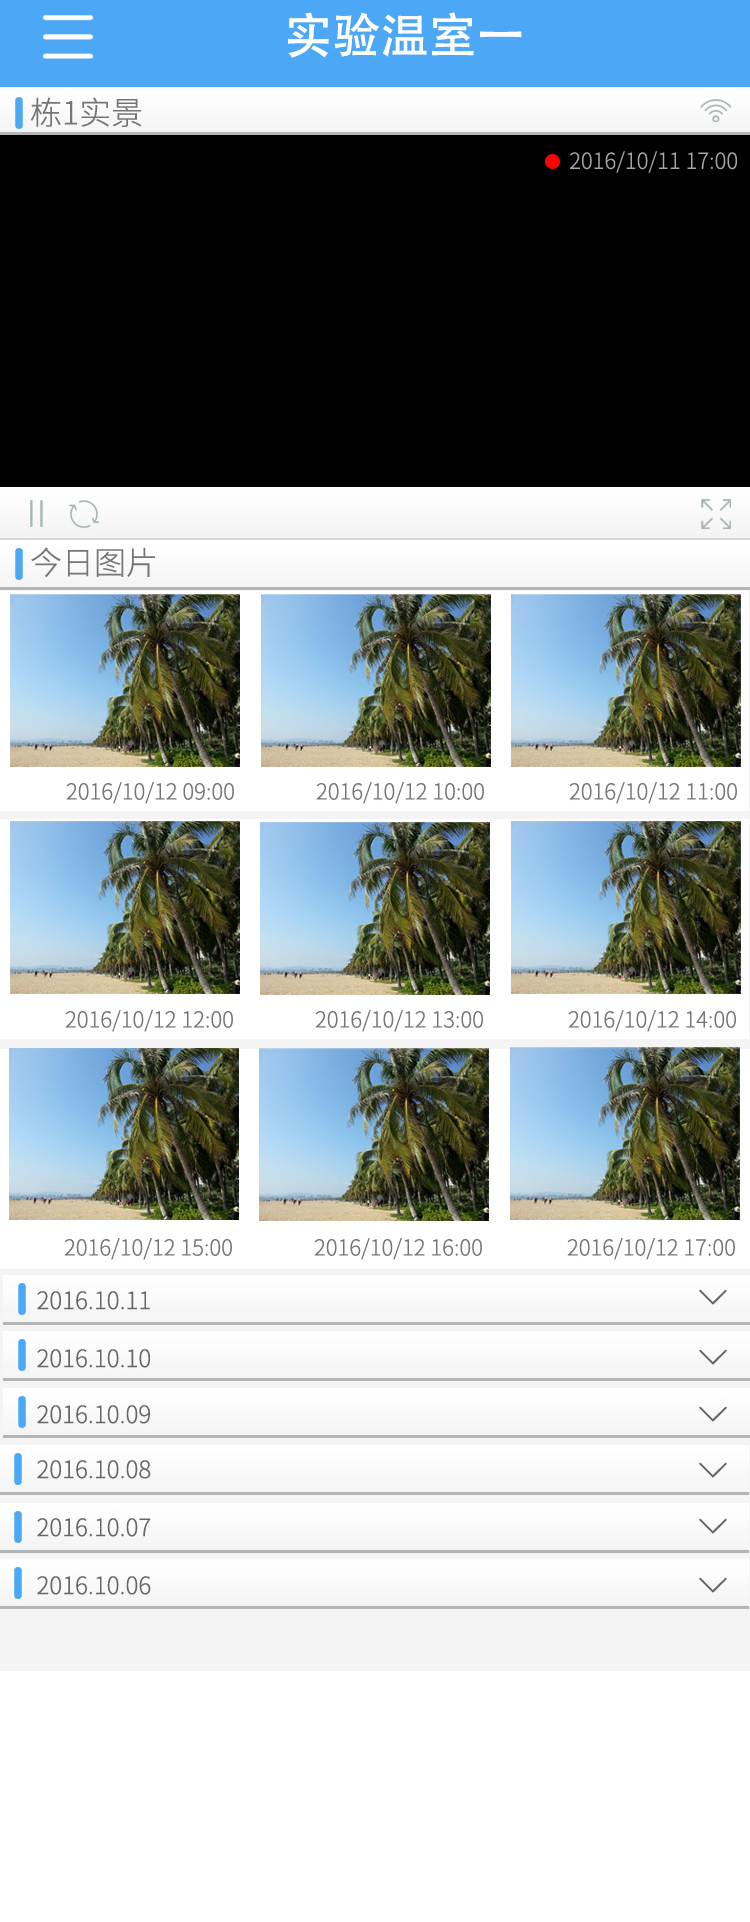
\includegraphics[width=0.18\textwidth]{UIDesign/video.jpg}
		}
		\subfigure[温室实景页]{
			\label{fig:ui:e}
			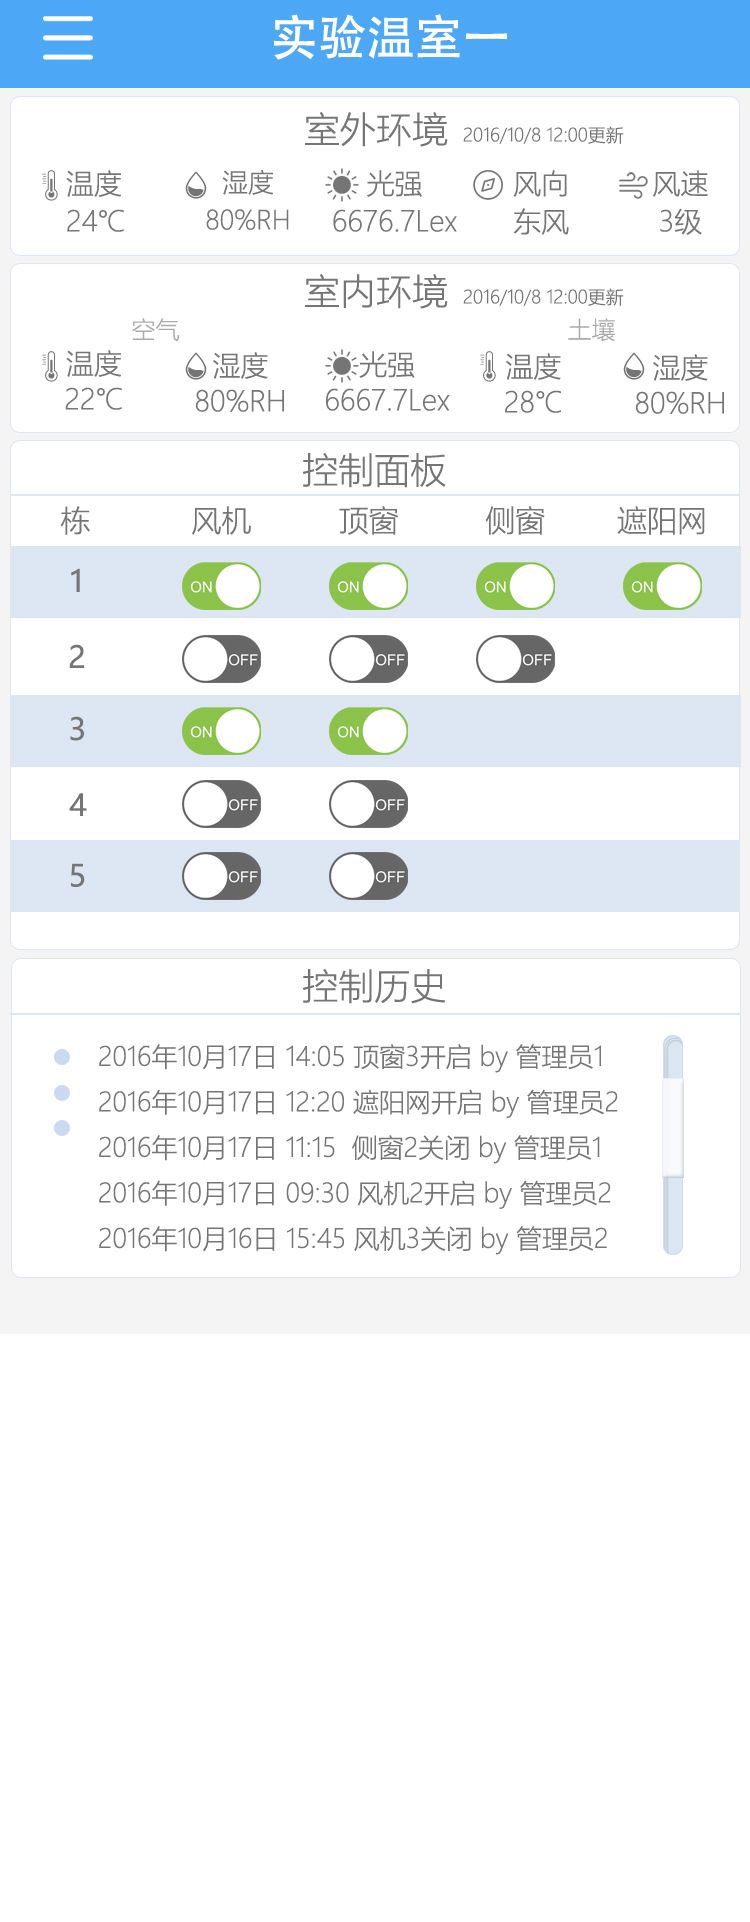
\includegraphics[width=0.18\textwidth]{UIDesign/control.jpg}
		}
	    \bicaption[fig:ui]{终端程序界面设计}{终端程序界面设计}{Fig}{UI design of the terminal program}
	\end{figure}
本次系统所有终端程序,包括WEB页面和移动客户端应用,均使用相同的UI和功能设计,设计图如图\ref{fig:ui}所示,主要分为温室选择页、温室详情页、历史曲线页、温室控制页、温室实景页等页面。

温室选择页,如图\ref{fig:ui:a}所示,用以显示所有的温室,并可选择任意温室进入。该页面上部可以查看当前温室地区的天气情况,下部列出所有的温室,并显示温室当前种植的作物图标、温室名称、温室类型、是否可以远程控制、是否有视频服务、是否有图像服务,以及温室当前的室内环境概况。

温室详情页,如图\ref{fig:ui:b}所示,用以显示所查看温室内的详细情况。该页面上部可查看当前温室室外环境参数,然后是温室室内的环境参数,若温室可控制则会显示温室作动器的控制状态,最下部显示温室当天的室内环境参数曲线。

历史曲线页,如图\ref{fig:ui:c}所示,该页显示温室一周内、一月内和所有近期的室内参数历史数据曲线,目前仅可查询一年内的数据曲线。

温室控制页,如图\ref{fig:ui:d}所示,如果温室可远程控制,则温室控制页可用,否则该页不可进入,用于远程控制温室内的作动器。该页面上部分别显示温室外和温室内的环境参数,中间为用于远程控制的按钮,下部为当前温室的控制历史日志。

温室实景页,如图\ref{fig:ui:e}所示,用于查看温室的当前视频和图像。如果温室视频服务可用的话则上部显示视频播放窗口,否则不显示;如果温室图像服务可用的话则显示近七天的图片,否则不显示,该部分图片既可以是温室摄像头自动捕获,也可以是人工上传;如果温室视频服务和图像服务都不可用则该页面不可进入。

	\subsection{本章小结}
本章按照系统架构设计的层次划分,以及各层次的概要设计,对每个层次进行了详细的设计,并基本实现完成。

感知控制层设计实现了传感器网络,包括硬件的设计和选型、传感器的选型、无线传感器网络的自定义协议及流程,同时对无线传感器网络节点进行了低功耗优化,使其能够满足农业生产环境恶劣、不易值守的特殊需求。另外完成了控制模块的硬件设计和选型,以及视频图像采集模块的设计和选型。

网络传输层主要实现了控制信息解析传输程序、数据采集上传程序和数据同步程序,搭建了感知控制层和上层系统之间的桥梁,使得温室环境监测数据能够稳定高效地采集并同步上传,控制指令能够稳定及时地下发。

应用层和终端接入层在商用云端服务器上搭建并配置了所需要的服务器端运行环境;基于Hadoop和MySQL搭建了农业物联网数据中心,解决了海量农业数据的存储和数据访问问题;使用Linux + Tomcat + Java的运行环境,基于Spring + Spring MVC + MyBatis的J2EE框架,构建了完整的服务器端程序;综合运用CFD仿真技术和机器学习技术设计了智能控制策略学习控制子系统,优化温室环境控制策略,以实现智能温室系统对温室环境的智能控制;使用Linux + Nginx的运行环境,基于HTML5 + CSS3 + JavaScript + AJAX技术构成,综合运用React、Redux、Webpack和Sass等技术,实现终端程序中WEB页面的开发,同时使用React Native实现移动端应用的开发,包括Android端和IOS端应用。
 %温室CFD仿真建模与验证
%# -*- coding: utf-8-unix -*-
%%==================================================
%% chapter0.tex for SJTU Master Thesis
%%==================================================


\chapter{温室CFD仿真建模与验证}
\label{chapter:CFD}
在夏季正午,由于室外气温明显高于作物的适宜生长温度,且太阳辐射量非常的大,遮阳网和自然通风已经无法完全满足温室的降温需求\supercite{Roy2005} ,此时需要通过打开风机和湿帘进行机械通风降温。虽然机械通风能实现高温条件下的有效降温\supercite{Norton2002,Kumar2009} ,但是机械通风设备成本较高,工作能耗较大,这就要求在温室设计阶段优化温室的结构参数和设备配置,在温室运行阶段实施有效降低能耗的优化控制策略。

温室面积往往较大,为了实现有效的环境监测,通常需要较多的监测点,这将带来较高的系统监测成本,同时农业物联网的特殊性也要求监测点的数量要控制在尽量少的范围内。

温室环境是一个流场、温度场、浓度场等多个物理场耦合在一起的多输入多输出的复杂大时延系统,各个环境变量之间相互影响,且一段时间后影响效果才会得以体现,导致对温室的监测和控制分析都非常困难,本章建立了温室CFD仿真模型,并通过实验对其进行了验证,仿真结果的分析为温室监测点的选择和控制策略的制定提供了理论依据。

\section{温室CFD仿真概述}
随着计算机性能和数值计算理论水平的飞速发展,CFD越来越多地应用到各种现代科研和工程应用中,它弥补了理论分析在研究比较复杂的问题中的限制性,解决了试验研究在研究过程中的局限性,同时可以避免大型试验所带来的巨大消耗。

CFD仿真本质上是利用计算机进行数值模拟计算,完成人力所难以完成的复杂计算过程,同时结合数据可视化技术将计算结果以图形或者动画的方式展示给研究人员。CFD计算的基本思想和流程即建立流动基本方程组,然后对其进行求解,从而实现对流体流动过程的数值模拟计算。

温室内是一个非常复杂的环境,多个物理场相互耦合在一起共同作用,不仅受到温室内外环境的变化的影响,还与温室的结构和作动器的动作有着密切的关系,且温室是一个大时延的系统,温室往往需要经过一段时间后,才会对环境变化或作动器动作有所反应。因此仅仅依靠传统的理论方法和试验方法难以解决温室内复杂的流场问题,CFD技术的发展,为温室内流场问题的研究带来了新的方法和手段。

OKUSHIMA等\supercite{Okushima1989} 首次应用CFD研究温室的通风问题,开拓了定量分析温室通风问题的有效途径。此后,随着CFD理论的不断完善和商用CFD软件的发展,温室通风CFD仿真结果已被证明具有良好的吻合性,计算速度也越来越满足生产的需要,研究效率大大提高。目前,CFD仿真已经成为进行温室通风研究的常用方法\supercite{Sase2004}。

在基于CFD的机械通风研究领域,随着仿真技术的发展和问题分析的深入,模型由二维到三维全尺度,由稳态分析到瞬态分析,由简单模拟到用于优化控制设计。BOURNETA等\supercite{Bournet2010}采用CFD方法研究了风机形状和安装方式对于温室内流体流动分布情况的影响。童莉等\supercite{TongLi2003} 建立了机械通风条件下的温室三维CFD模型,研究了温室气温可控距离与入口风速和湿帘安装高度之间的关系。CHEN等\supercite{Chen2014} 采用CFD方法研究了湿帘、风机安装位置与湿帘-风机系统降温效果之间的关系。胥芳等\supercite{XuFang2015} 采用CFD 方法分析了不同温室长度、湿帘入口面积和风机转速对于温室降温的影响,并根据分析结果提出了优化方案。任守纲等\supercite{RenShougang2015} 基于CFD方法建立了夏季温室气温变化瞬态模型,研究了自然通风和机械通风降温措施切换控制策略。

通过本文设计实现的智能温室监测与控制系统,使得根据当前温室内外的环境参数对温室机械通风实时控制成为可能,从而更有效地提高机械通风效率、降低运行能耗。在温室机械通风实施优化控制的过程中,需要选择合理的监测点位置,获取机械通风效果与各工作参数之间的定量关系。由于实际工作环境的不可重复性,温室CFD仿真比实验能更有效地确定机械通风效果与控制参数之间的关系。温室机械通风是典型动态过程,但目前对于机械通风瞬态过程的实验和仿真研究还不够深入,因此本文建立全尺度三维瞬态和稳态CFD仿真模型,反映机械通风作用下,温室内空气温度的时空分布和变化过程,用以评价机械通风效果、选择合适的监测点位置方案、优化风机的控制策略。


\section{温室环境CFD建模}
	\subsection{理论基础}
		\subsubsection{基本控制方程}
所有的流体流动都遵循基本的守恒定律,包括质量守恒定律、动量守恒定律、能量守恒定律,对于多组分的流体流动还需要遵循组分守恒定律。

自然任何自然现象,包括流体流动,都满足质量守恒定律,由质量守恒定律可以得到质量守恒方程,也称为连续性方程,如式\ref{eqn:zhiliang}所示\supercite{ComsolCfd2015,WangFujun2004} :
	\begin{equation}
		\label{eqn:zhiliang}
		\frac{\partial\rho}{\partial t}+\frac{\partial \rho u}{\partial x}+\frac{\partial \rho v}{\partial y}+\frac{\partial \rho w}{\partial z}=0
	\end{equation}

引入散度符号$\nabla$可表示为式\ref{eqn:zhiliang1}
	\begin{equation}
		\label{eqn:zhiliang1}
		\frac{\partial\rho}{\partial t}+\nabla \cdot (\rho \mathbf{u}) =0
	\end{equation}
其中$\rho$为流体密度,$t$为时间,$\mathbf{u}$为速度矢量。

对于不可压流体,密度$\rho$可看作常数,可得式\ref{eqn:zhiliangRho};对于稳态流动,密度$\rho$不随时间变化,可得式\ref{eqn:zhiliangRhoCon}。
	\begin{equation}
		\label{eqn:zhiliangRho}
		\nabla \cdot \mathbf{u} =0
	\end{equation}
	\begin{equation}
		\label{eqn:zhiliangRhoCon}
		\nabla \cdot (\rho \mathbf{u}) =0
	\end{equation}
动量守恒定律也是任何流体流动都必须遵循的基本物理定律,由该定律可得$x$、$y$、$z$三个方向的动量守恒方程如\ref{eqn:dongliang} 所示\supercite{ComsolCfd2015,WangFujun2004} :
	\begin{equation}
		\label{eqn:dongliang}
		\left\{
		\begin{aligned}
		\frac{\partial \rho u}{\partial t}+\nabla \cdot (\rho u \mathbf{u}) = - \frac{\partial \rho}{\partial x}+\frac{\partial \tau_{xx}}{\partial x}+\frac{\partial \tau_{yx}}{\partial y}+\frac{\partial \tau_{zx}}{\partial z} + F_x \\
		\frac{\partial \rho v}{\partial t}+\nabla \cdot (\rho v \mathbf{u}) = - \frac{\partial \rho}{\partial y}+\frac{\partial \tau_{xy}}{\partial x}+\frac{\partial \tau_{yy}}{\partial y}+\frac{\partial \tau_{zy}}{\partial z} + F_y \\
		\frac{\partial \rho w}{\partial t}+\nabla \cdot (\rho w \mathbf{u}) = - \frac{\partial \rho}{\partial z}+\frac{\partial \tau_{xz}}{\partial x}+\frac{\partial \tau_{yz}}{\partial y}+\frac{\partial \tau_{zz}}{\partial z} + F_z 
		\end{aligned}
		\right.
	\end{equation}
其中$p$为流体微元体上的压力,$\tau_{ii}$为作用在微元体表面上的黏性应力的分量,$F_x$、$F_y$、$F_z$为微元体上的体积力,在只存在重力的情况下,且规定$z$轴竖直向上时,则有$F_x=0$、$F_y=0$、$F_z=\rho g$。

对于牛顿流体,黏性应力与流体的变形率成比例,可得如下动量守恒方程,即著名的Navier-Stokes(N-S)方程,如\ref{eqn:ns} 所示\supercite{WangFujun2004} :
	\begin{equation}
		\label{eqn:ns}
		\left\{
		\begin{aligned}
		\frac{\partial \rho u}{\partial t}+\nabla \cdot (\rho u \mathbf{u}) =- \frac{\partial \rho}{\partial x}+\nabla \cdot (\mu \nabla \cdot u ) + S_x \\
		\frac{\partial \rho v}{\partial t}+\nabla \cdot (\rho v \mathbf{u}) =- \frac{\partial \rho}{\partial y}+\nabla \cdot (\mu \nabla \cdot v ) + S_y \\
		\frac{\partial \rho w}{\partial t}+\nabla \cdot (\rho w \mathbf{u}) =- \frac{\partial \rho}{\partial z}+\nabla \cdot (\mu \nabla \cdot w ) + S_z 
		\end{aligned}
		\right.
	\end{equation}
其中,$\mu$为动力黏度,$S_x$、$S_y$、$S_z$为方程的广义源项,有 $S_x=F_x+s_x$、$S_y=F_y+s_y$、$S_z=F_z+s_z$,一般情况下,$s_x$、$s_y$、$s_z$都为小量,对于不可压流体,$s_x=s_y=s_z=0$。

对于存在能量交换的物理问题还必须遵循能量守恒定律,存在能量交换的流体流动问题也是如此,由该定律可得能量守恒方程,对于牛顿流体,如\ref{eqn:heat}所示\supercite{ComsolHeat2015,WangFujun2004} :
	\begin{equation}
		\label{eqn:heat}
		\rho C_p (\frac{\partial T}{\partial t}+(\mathbf{u} \cdot \nabla) T + \nabla \cdot \mathbf{q}  =Q
	\end{equation}
其中$C_p$为恒压比热容,$T$为热力学温度,$\mathbf{q}$为热通量矢量,$Q$为能量源项。

对于存在物质交换的流体流动问题中,每种组分还必须要满足组分守恒定律,由该定律可得组分守恒方程,如式\ref{eqn:conc} 所示\supercite{ComsolChem2015,WangFujun2004} :
	\begin{equation}
		\label{eqn:conc}
		\frac{\partial c_i}{\partial t}+\mathbf{u} \cdot \nabla c_i = \nabla \cdot (D_i \nabla c_i ) + R_i
	\end{equation}
其中$c_i$为组分$i$的浓度,$D_i$为组分$i$的扩散系数,$R_i$为单位时间内系统内单位体积通过化学反应生成的组分$i$的量。
		\subsubsection{温室流体流动问题的简化}
研究表明,对于气体流速较小,一般为50 m/s以下,压强梯度不大时,气体流体可以看作不可压流体。通常情况下,温室内植物生产区域的气流速度不宜过高,一般低于2 m/s,因此温室中的流体为低速流动,可看作不可压流体。另外,在仿真中可以假设温室内气体为连续、稳定的牛顿流体,并忽略黏性发热和压力功。而且一般可假设气体的各组分之间无化学反应。

		\subsubsection{湍流模型的选择}
湍流是一种即使边界条件不发生变化,流动也处于不稳定的状态,各个流动相关的变量随机发生变化。根据流动实验结果,当雷诺数(Reynolds数,简称Re数)大于另一个临界值时,流体流动将变得混乱,出现不同尺度的涡,此时流体流动为湍流。

在温室内,由于温室尺寸往往较大,温室内流体流动的Re数较大,根据相关文献,温室内自然对流即呈现出湍流状态,机械通风情况下Re数更大,更加呈现出高度湍流。因此,在温度分布不均匀和机械通风的共同作用下,以及流体受边界的限制,温室内的气体流动可看作是湍流流动\supercite{WangFujun2004} 。

对于湍流的数值计算目前有直接数值计算和非直接数值计算两种。

直接数值计算即为直接用流动控制方程对湍流进行求解计算,可以得到最真实的理论解,得到的结果也是最精确的,但是该方法对于计算机的性能要求非常高,目前只能用来求解比较简单的问题,对于复杂的工程问题还不具有现实工程意义。

目前,非直接数值计算对于解决实际工程问题使用最为广泛的为Reynolds平均法,该方法可以用相对小的计算量得到相对精确的计算结果。

本文选用工程上广泛使用的Reynolds平均法中的标准$k-\varepsilon$湍流模型进行温室通风仿真\supercite{Sase2004,RenShougang2015,WuFeiqing2010} 。该模型引入了湍动能$k$方程,如式(9)所示,和湍流耗散率$\varepsilon$方程,如式(10)所示。
	\begin{equation}
		\label{eqn:k}
		\rho \frac{\partial k}{\partial t}+\rho \mathbf{u} \cdot \nabla k = \nabla \cdot ((\mu + \frac{\mu_t}{\sigma_k}) \nabla k) -\rho \varepsilon +P_k
	\end{equation}
	\begin{equation}
		\label{eqn:e}
		\rho \frac{\partial \varepsilon}{\partial t}+\rho \mathbf{u} \cdot \nabla \varepsilon = \nabla \cdot ((\mu + \frac{\mu_t}{\sigma_{\varepsilon}}) \nabla \varepsilon ) +C_{\varepsilon 1} \frac{\varepsilon}{k} P_k - C_{\varepsilon 2} \rho \frac{\varepsilon^2}{k}
	\end{equation}
其中$C_{\mu}$、$C_{\varepsilon 1}$、$C_{\varepsilon 2}$、$\sigma_k$、$\sigma_{\varepsilon}$为常数,$\mu_t =\rho C_{\mu} \frac{k^2}{\varepsilon}$,
$P_k=\mu_t(\nabla \mathbf(u):(\mathbf(u)+(\mathbf(u))^T))-\frac{2}{3}(\nabla \mathbf(u))^2)-\frac{2}{3}\rho k \nabla \cdot \mathbf(u)$。

但是标准 湍流模型是针对充分发展的湍流流动建立的,不适用于湍流发展不充分的近壁面区域,因此需要引入壁面函数法解决该问题\supercite{WangFujun2004}。壁面函数法即在湍流核心区采用标准$k-\varepsilon$湍流模型求解,而在壁面区借助一组半经验公式,将壁面区与核心区的求解变量关联起来,这样不用对壁面区进行求解也可以得到与壁面区域相邻节点的变量值了。
	\subsection{仿真软件}
	目前对于CFD仿真计算,比较常见的计算仿真软件有FLUENT、CFX、COMSOL Multiphysics等,但是FLUENT、CFX等均作为CFD计算求解器存在,还需要配合GAMBIT等前处理软件和TECPLOT等后处理软件使用,COMSOL Multiphysics提供整个流程的解决方案,几何建模、前处理、求解和后处理之间无缝结合,因此本文CFD仿真使用COMSOL Multiphysics 5.2作为仿真软件。
	
COMSOL Multiphysics是当今世界第一款真正的任意多物理场直接耦合分析软件,计算快速高效精确,采用完全开放的架构,可以轻松地自定义专业的偏微分方程,而无需使用复杂的UDF开发,可以实现任意求解参数的独立函数控制,拥有丰富的后处理功能,可以根据需要进行任意数据、曲线、图片及动画的生成及导出,且支持跨平台计算和并行计算\supercite{Comsol2015}。

	\subsection{几何建模}
本文CFD仿真研究对象为我国南方典型连栋塑料温室,位于上海市崇明岛(E121.74°,N31.50°),温室如\ref{fig:House}所示。
	\begin{figure}[!htbp]
		\centering
		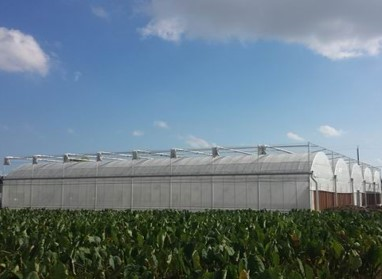
\includegraphics[width=0.3\textwidth]{15House.png}
		\bicaption[fig:House]{南方连栋塑料温室}{南方连栋塑料温室}{Fig}{Multi-span plastic greenhouse in Southern China}
	\end{figure}
温度顶高5 m,肩高3 m,屋脊方向为东西走向,长度32 m,单栋跨度8 m,共5栋,总宽度40米。温室西墙安装湿帘,湿帘高度为1.8 m,中心位置安装高度为1.3 m,每套长度为17 m,温室南北两侧各一套,中间为2 m宽的推拉门。温室东墙安装10台YS1250型重锤式负压风机,每栋两台,风机直径为1250 mm,中心位置安装高度为1.5 m,电机功率为1.1 kW,单台排风量 为40000 m3/h。温室主体采用结构钢,四周及顶部覆盖聚乙烯薄膜,薄膜厚度为0.15 mm,透光率大于(等于)90%,顶部安装遮阳网,采用专用优质缀铝外遮阳网布,遮阳率可达80\%。

在COMSOL Multiphysics中按照1:1的比例建立温室的几何模型,如\ref{fig:Geometrical}所示。
	\begin{figure}[!htbp]
		\centering
		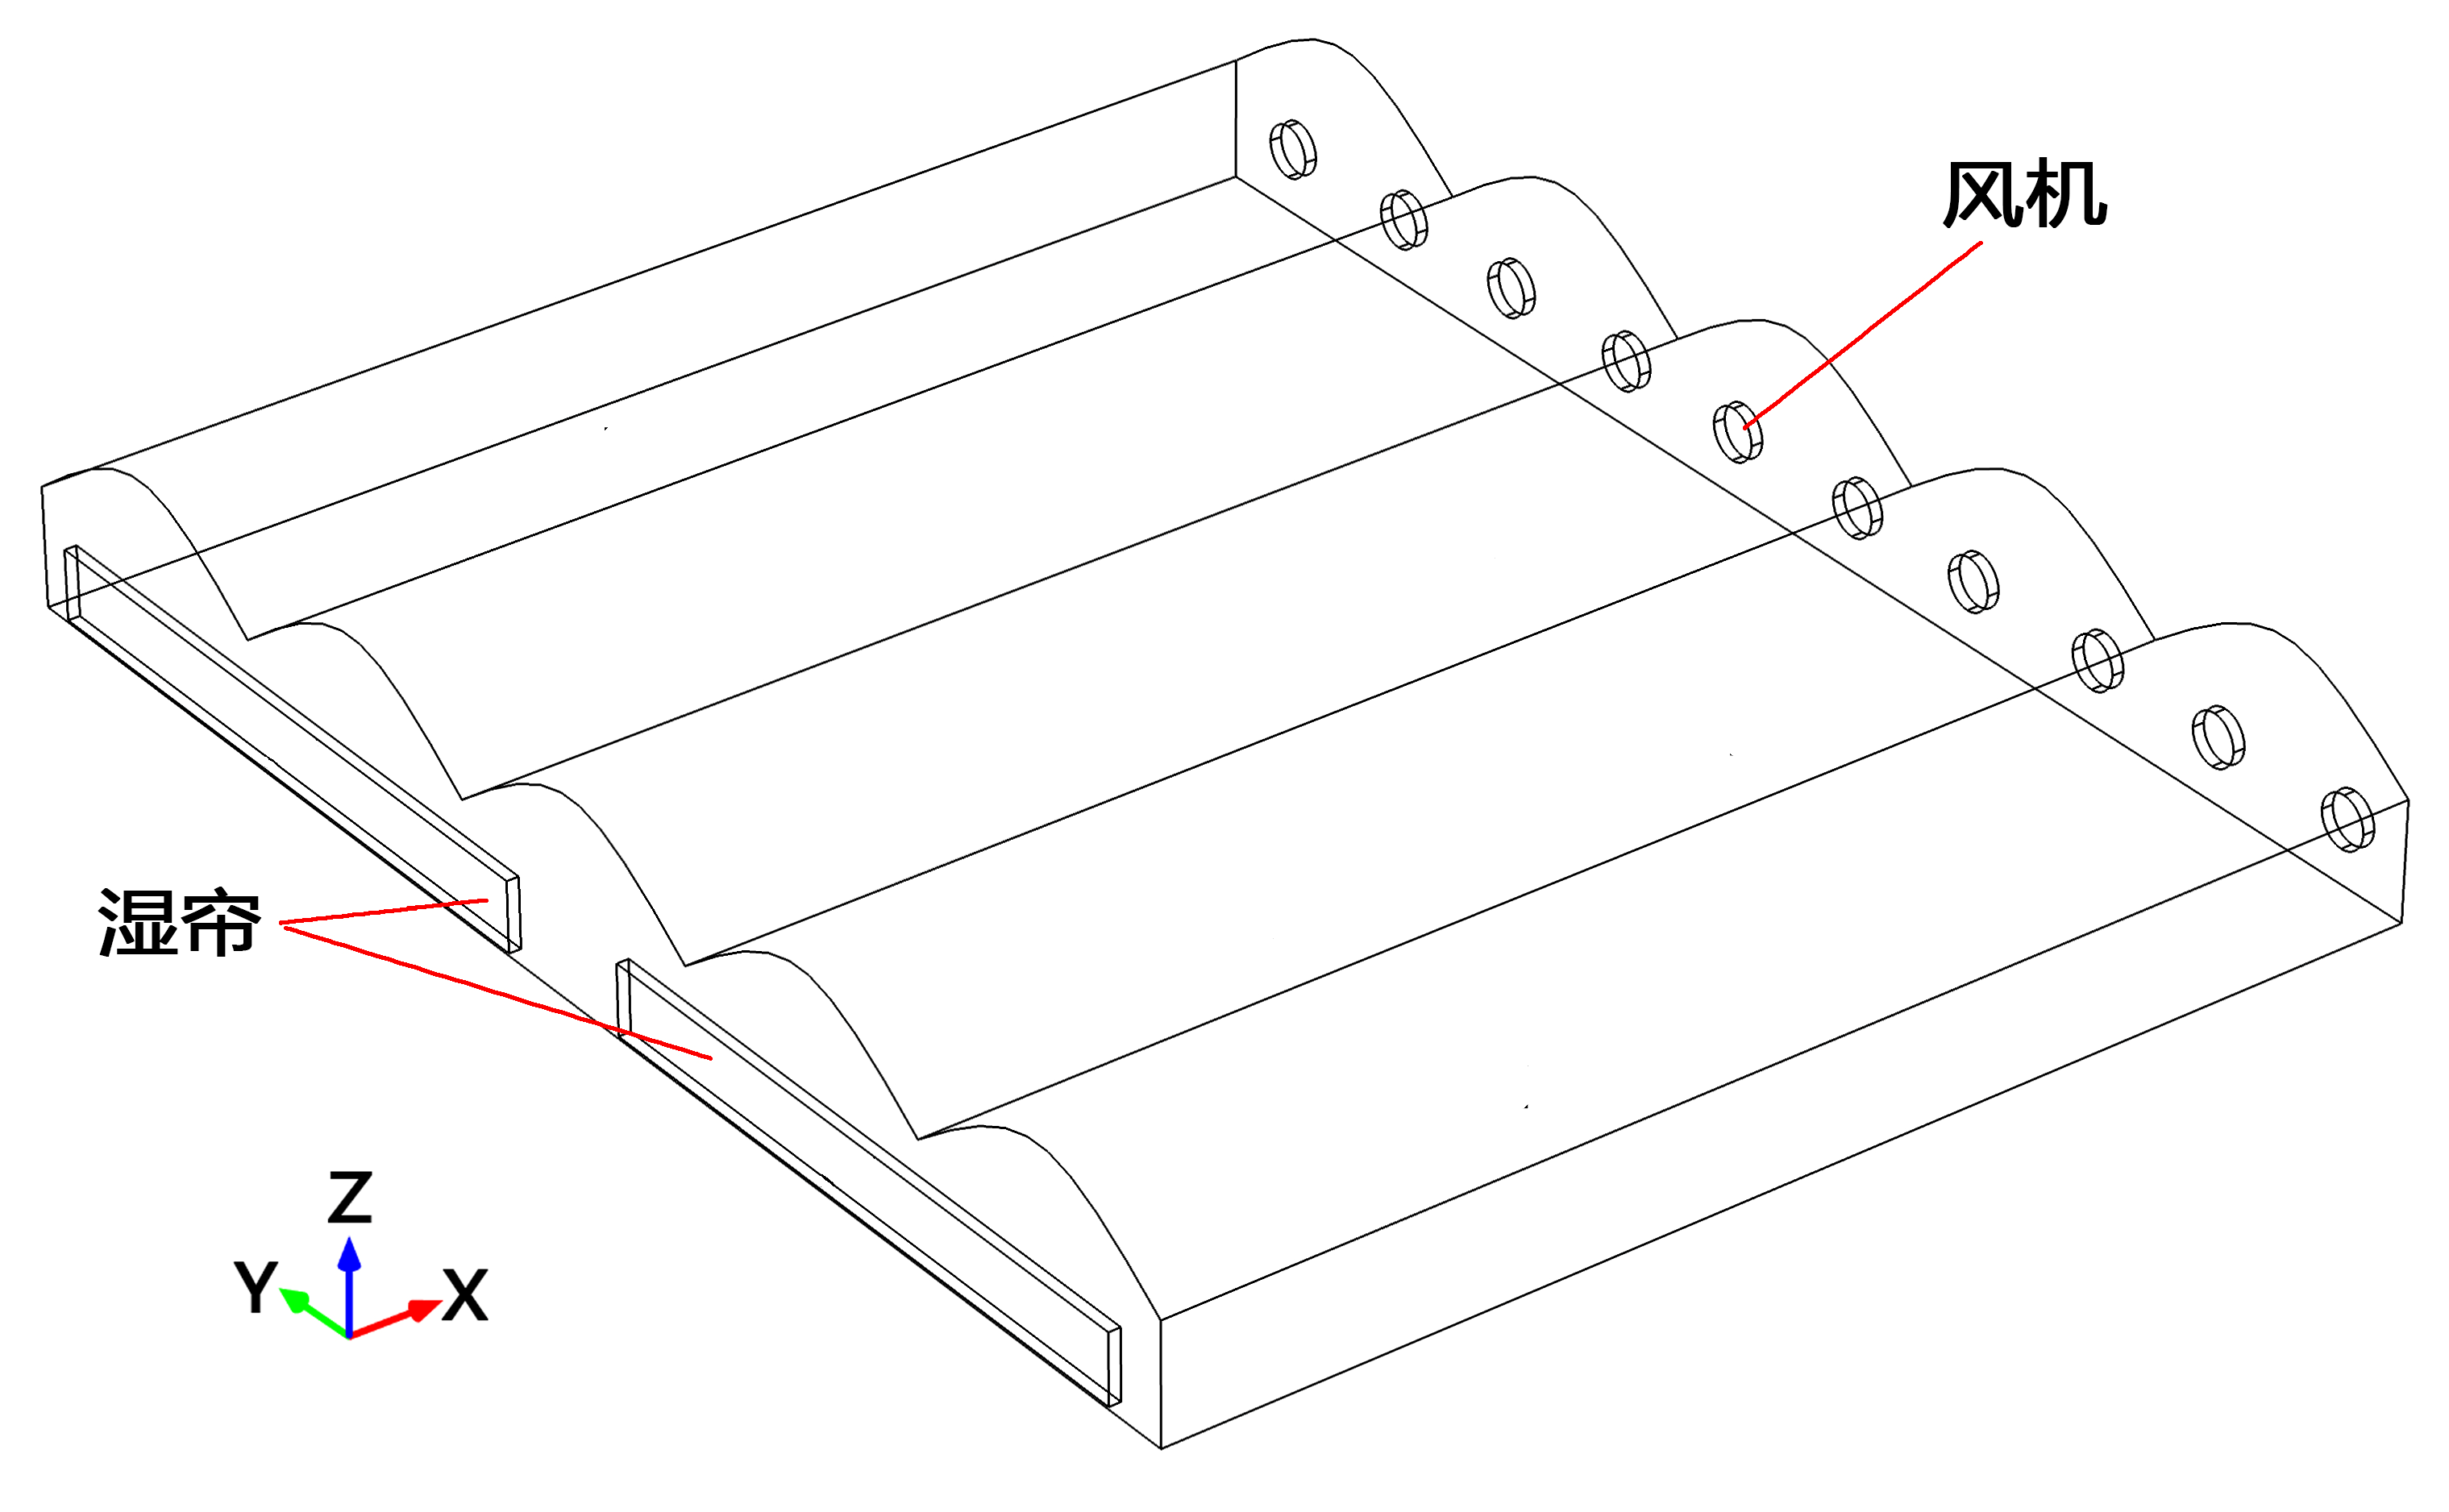
\includegraphics[width=0.7\textwidth]{16Geometrical.png}
		\bicaption[fig:Geometrical]{温室几何模型}{温室几何模型}{Fig}{Geometrical model of the greenhouse}
	\end{figure}
本模型为减少计算量,提高计算速度,根据研究侧重点和温室特点对温室几何模型做出如下合理的简化:
	\begin{enumerate}
		\item 温室表面的薄膜厚度仅有0.15 mm,在模型中可以忽略不计,因此几何模型中简化为无厚度的面。
		\item 由于侧窗、顶窗和门在机械通风过程中均为关闭状态,对温室机械通风过程不起作用,且会增加网格数量,同时影响网格的划分质量,因此几何模型忽略了它们的细节建模。
		\item 温室内的支撑结构和排水沟相较温室尺寸较小,对通风过程影响较小,且会急剧增加网格的数量,使计算速度缓慢,因此在建模过程中忽略。
		\item 温室外遮阳网通过太阳辐射强度折减来体现,不体现在几何模型中。
		\item 实验期间温室内种植高度低于20 cm的西瓜和甜瓜,因此忽略其几何建模\supercite{HeKeshi2012,RenShougang2015} 。
	\end{enumerate}
	
	\subsection{多物理场}
	机械通风条件下,温室内气温的时空分布和变化受室内外环境条件、湿帘-风机、太阳等因素的影响。因此,需要在COMSOL中添加多个物理场模块。
	
首先为解决流场问题,在软件中流体流动模块下添加单相流-湍流-湍流, 模块;然后因为温室仿真中涉及到流体传热,在软件中传热模块下添加流体传热模块;最后考虑到湿帘和水分蒸发对于温室中环境的影响,在软件中化学物质传递模块下添加稀物质传递模块。

为建立各个物理场模块之间的耦合关系,对各个模块之间做如下处理:
	\begin{enumerate}
		\item 湍流模块和稀物质传递模块之间通过速度、绝对压力和浓度耦合;
		\item 湍流模块和流体传热模块之间通过速度、绝对压力和温度耦合;
		\item 稀物质传递模块和流体传热模块之间通过浓度耦合。
	\end{enumerate}
为了引入流体传热模块对流体密度和黏度的影响,在多物理场选项下添加非等温流模块。

	\subsection{边界条件}
	为获得温室机械通风过程的初始状态,从而研究机械通风过程及其升温过程,本文仿真过程分为湿帘风机关闭状态和开启状态。前者温室处于密闭环境,风机和湿帘处于关闭状态,用以计算自然对流状态下温室内的状态;后者风机和湿帘处于开启状态,进行机械通风过程仿真,用以计算湿帘风机对温室内环境分布和变化的影响。
	
本次仿真以温室内的空气为主要研究对象,所涉及的边界条件包括室外环境参数、温室四周薄膜和顶棚、风机、湿帘、室内地面等,设置见\ref{tab:boundary}。由于关注的仿真过程时间较短,故可以忽略在此期间内各边界条件基本参数的变化,各算例基本参数设置见\ref{tab:basicParameters}。
		\begin{table}[!htbp]
  			\centering
  			\bicaption[tab:boundary]{CFD模型边界条件}{CFD模型边界条件}{Table}{Boundary condition used in the CFD model}
  			\begin{tabular}{ccccc} \toprule
			类型	 & 边界 & 湍流场 & 	流体传热 & 	稀物质传递\\ \midrule
			\multirow{5}{*}{关闭风机} & 四周围护 & 壁面 & 热通量、散射面 & 无通量\\ 
												  & 顶棚  & 壁面 & 热通量、散射面 & 无通量\\
												  & 地面 & 壁面 & 温度、散射面 & 无通量\\
												  & 风机 & 壁面 & 热通量、散射面 & 无通量\\
												  & 湿帘 & 壁面 & 热通量、散射面 & 无通量\\ \midrule
			\multirow{5}{*}{开启风机} & 四周围护 & 壁面 & 热通量、散射面 & 无通量\\
												  & 顶棚 & 壁面	 & 热通量、散射面	 & 无通量\\
												  & 地面 &  壁面 & 温度、散射面	 & 无通量\\
												  & 风机 &  压力出口 & 	流出 & 	流出\\
												  & 湿帘 & 速度入口	 & 温度 & 浓度\\ \bottomrule
 			\end{tabular}
		\end{table}	
		\begin{table}[!htbp]
  			\centering
  			\bicaption[tab:basicParameters]{基本参数设置}{基本参数设置}{Table}{Common parameters in the CFD model}
  			\begin{tabular}{cc} \toprule
			参数 & 数值\\ \midrule
			太阳辐射强度/(W·m-2) & 	832\\
			室外环境温度/℃	 & 36.5\\
			室内地面温度/℃ & 	39.5\\
			入口相对湿度/\%	 & 82.3\\
			薄膜壁面温度/℃	 & 39.5\\
			薄膜顶棚温度/℃	 & 41.5\\
			薄膜对流换热系数/(W·(m2·K)-1) & 6.6\\
			土壤发射率 & 0.92\\
			薄膜发射率 & 0.7\\
			土壤吸收率 & 0.88\\
			薄膜吸收率 & 0.1\\ \bottomrule
 			\end{tabular}
		\end{table}
湿帘风机关闭状态下,即计算自然对流状态时,还需对温室整个计算域设置体积力域,用以计算空气密度因为受温度变化影响而带来的自然对流,并设置压力约束点以提供压力参考点。

湿帘风机开启状态下,即计算机械通风过程时,入口风速计算\supercite{RenShougang2015}见式\ref{eqn:input}:
	\begin{equation}
		\label{eqn:input}
		v_{in} = \frac{n Q_{fan}}{S_{in}}
	\end{equation}
其中$v_{in}$为入口风速,$n$为开启风机的数量,$Q_{fan}$为单台风机的排风量,$S_{in}$为湿帘入口总面积。

入口温度可根据湿帘降温模型计算\supercite{JBT}见式\ref{eqn:cool}:
	\begin{equation}
		\label{eqn:cool}
		T_{in}=T_{out}-E (T_{out} - T_{w})
	\end{equation}
其中$T_{in}$为湿帘后干球温度,$T_{out}$为湿帘前干球温度,$E$为湿帘蒸发冷却换热效率,$T_w$为湿帘前湿球温度。

	\subsection{网格划分和求解步骤}
为研究机械通风条件下,整个温室内的空气温度时空分布和变化,本文CFD仿真计算选取整栋温室作为计算域。模型内部大部分区域采用自由剖分四面体网格进行划分,并在入口、出口和壁面边界处进行边界层加密,以适应该区域速度、温度和浓度梯度变化大的要求。为得到数值计算的网格无关解,反复尝试不同密度的网格,本次计算整个模型共划分743604域单元、59854边界单元和 2424边单元,如\ref{fig:Mesh}所示。
	\begin{figure}[!htbp]
		\centering
		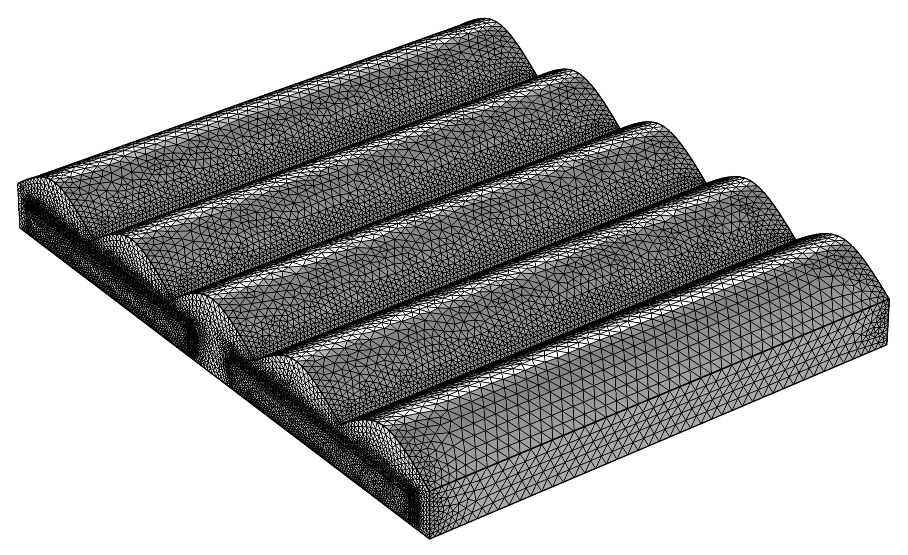
\includegraphics[width=0.5\textwidth]{17Mesh.png}
		\bicaption[fig:Mesh]{温室CFD模型网格划分}{温室CFD模型网格划分}{Fig}{Mesh of the greenhouse CFD model}
	\end{figure}
本次仿真计算划分为若干个阶段:

第1阶段进行湿帘风机关闭状态下的稳态求解,此阶段用以计算自然对流状态下温室内状态分布,为进行机械通风的仿真计算获得初始值,此阶段使用稳态求解器进行求解;

第2阶段进行湿帘风机开启状态下的瞬态求解,求解变量的初始值设为第1阶段的计算解,此阶段使用瞬态求解器进行求解;

随后每个阶段都以上阶段的计算结果作为初始值进行稳态或瞬态任意状态的仿真计算。各阶段之间的求解计算主要关注速度、绝对压力、温度、浓度等关键参数的传递。

本文所有CFD仿真计算均在Intel Xeon E5-1620V3 四核心CPU,主频3.5GHz,内存64GB,操作系统为Windows10 x64的小型工作站上进行,CFD仿真建模过程中前处理、求解、后处理等过程均在COMSOL Multiphysics 5.2环境下进行。各算例稳态计算历时近6 h完成,瞬态计算与仿真步长和时长有关,如步长1.5 s时长10 min历时近15 h完成。

\section{机械通风实验}
	\subsection{实验平台}
本次实验的实验平台为本文设计并实现的智能温室系统,通过该系统平台实现室内的空气温湿度、土壤温湿度的测量,和室外的空气温湿度、太阳辐射强度等的测量。
	
部分无需长期监测的数据如土壤表面温度和薄膜表面温度,本次实验采用单独的设备进行测量。土壤表面温度的测量采用CA380型手持红外测温仪,测量范围为-32~380℃,测量精度为±2℃;薄膜表面温度测量采用铂电阻PT100,测量范围为-200~200℃,测量精度为±0.15℃。

	\subsection{实验方案}
一般情况下,七月下旬至八月上旬,上海地区的气温达到全年的最高值,该段时间内对于温室的降温尤为重要。本次实验的实验时间为2016年7月31日,天气晴朗,室外温度较高且相对平稳。实验开始时间为13:10,温度为一天中最高的阶段,室外气温达到36℃以上,此时仅依靠自然通风等手段已经无法将温度降至32℃以下。研究表明,室内气温达到32℃以上将对作物的生长产生较大的影响,此时需要开启湿帘-风机进行机械通风降温。实验期间温室外遮阳网保持打开。
	\begin{figure}[!htbp]
		\centering
		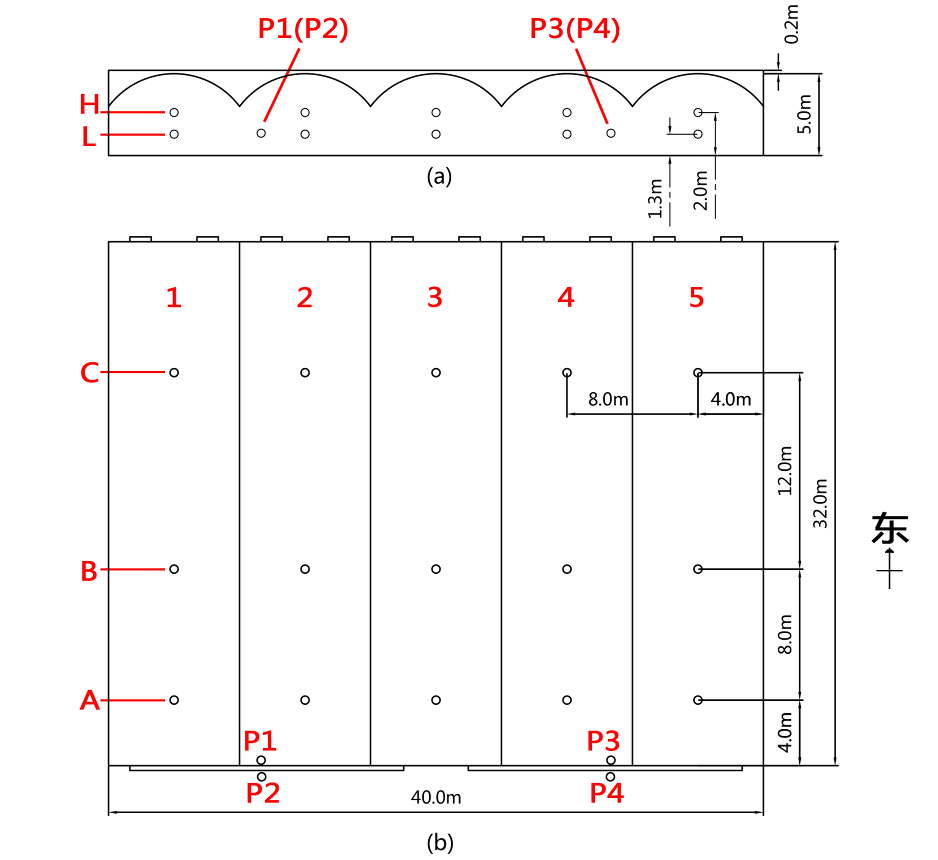
\includegraphics[width=0.7\textwidth]{18Distribution.png}
		\bicaption[fig:Distribution]{温室内传感器节点分布图}{温室内传感器节点分布图}{Fig}{Distribution of sensors in the greenhouse}
	\end{figure}
实验期间,温室内所有传感器测点每20 s记录一次数据。温室内外共布置30个测量节点,具体分布如\ref{fig:Distribution}所示。传感器编号方式如\ref{fig:Distribution}所示,距离湿帘4、12、24 m位置处分别编号A、B、C,距离地面1.3 m和2 m位置处分别编号H、L,自北向南每栋编号1、2、3、4、5,除HA1、HC1、HA5、HC5外,其余位置各布置一个节点;另外分别在紧邻湿帘内外正中间位置处,东西两侧各布置一个节点,如\ref{fig:Distribution}所示的P1、P2、P3、P4点。为避免温室等建筑物对于室外气象站的影响,室外气象站布置在距离温室10 m处的空旷区域,安装在距离地面10 m处的位置,距离温室较远且体积较小,因此未在图中标出。

	\subsection{实验步骤}
根据实验方案,本次实验分别进行了开启关闭10台、6台和4台风机的机械通风实验。
	
每组实验采用相同的实验步骤:
	\begin{enumerate}
		\item 实验前的准备工作,检查所有实验设备,确保所有设备正常工作,完成温室的密封性检查,并将温室缝隙补上。
		\item 关闭所有门窗,待温室内气温升高至稳定。
		\item 打开湿帘处的卷帘,开启风机,待温室内气温降低至稳定。
		\item 关闭风机,关闭湿帘处的卷帘,待温室内气温升高至稳定。
		\item 重复上述步骤,进行下一组实验。
	\end{enumerate}
	
	\subsection{实验结果}
	本文选取最具代表性的先后开启和关闭10台和4台风机情况下植物冠层即截面L典型位置处的实验结果进行分析,实验测得的温室内气温变化曲线如图23所示。
	\begin{figure}[!htbp]
		\centering
		\subfigure[截面2温度实测值]{
			\includegraphics[width=0.8\textwidth]{result/01.png}
		}
		\subfigure[截面B温度实测值]{
			\includegraphics[width=0.8\textwidth]{result/02.png}
		}
		\subfigure[风机开启情况]{
			\includegraphics[width=0.8\textwidth]{result/03.png}
		}
 		\bicaption[fig:Result]{温室内植物冠层温度实测值}{温室内植物冠层温度实测值}{Fig}{Measured temperature inside the greenhouse at Section L}
 	\end{figure}
	如\ref{fig:Result}所示,由实验结果曲线可以看出,对于开启10台和4台风机的情况,各测点空气温度变化趋势基本一致,即开启风机时首先快速下降,随后缓慢下降,最后达到最低温度,并保持稳定。两者的差别体现在,开启10台风机的情况下,相较于开启4台风机的情况,空气温度下降速度较快,且纵向温度梯度较大,最终达到的稳定温度略低,横向分布较为均匀。关闭风机后,两种情况的空气温度上升趋势基本一致。
	
图\ref{fig:Result}所示为屋脊方向典型纵截面,即如\ref{fig:Distribution}所示截面2的实验结果,该截面的结果可以观察到与湿帘不同距离测点空气温度的变化情况,从结果中可以看出距离湿帘越近,空气温度下降越早,且最终达到的稳定温度越低。

图\ref{fig:Result}所示为温室跨度方向典型横截面,即如\ref{fig:Distribution}所示截面B的实验结果,该截面的结果可以观察到每栋内测点空气温度的变化情况,可以看出受推拉门处造成的湿帘不连续的影响,第3栋降温效果最差,空气温度下降速度最慢,且最终达到的稳定温度最高。

\section{模型验证}
模型验证时选取实验参数作为边界条件参数,具体参数见\ref{tab:cases}中Case 1的参数设置,即开启风机数量为10台,入口温度为30℃,温室长度为32 m,其它基本参数设置如表5所示。实验条件下,温室内植物冠层即截面L的典型截面即截面2和截面B中的各测点空气温度仿真值和实测值如图24所示,由于截面B具有对称性,因此图中仅展示B1、B2、B3测点结果。
	\begin{figure}[!htbp]
		\centering
		\subfigure[截面2仿真值]{
			\label{fig:Compare:a}
			\includegraphics[width=0.4\textwidth]{compare/01.png}
		}
		\subfigure[截面2实测值]{
			\label{fig:Compare:b}
			\includegraphics[width=0.4\textwidth]{compare/02.png}
		}
		\subfigure[截面B仿真值]{
			\label{fig:Compare:c}
			\includegraphics[width=0.4\textwidth]{compare/03.png}
		}
		\subfigure[截面B实测值]{
			\label{fig:Compare:d}
			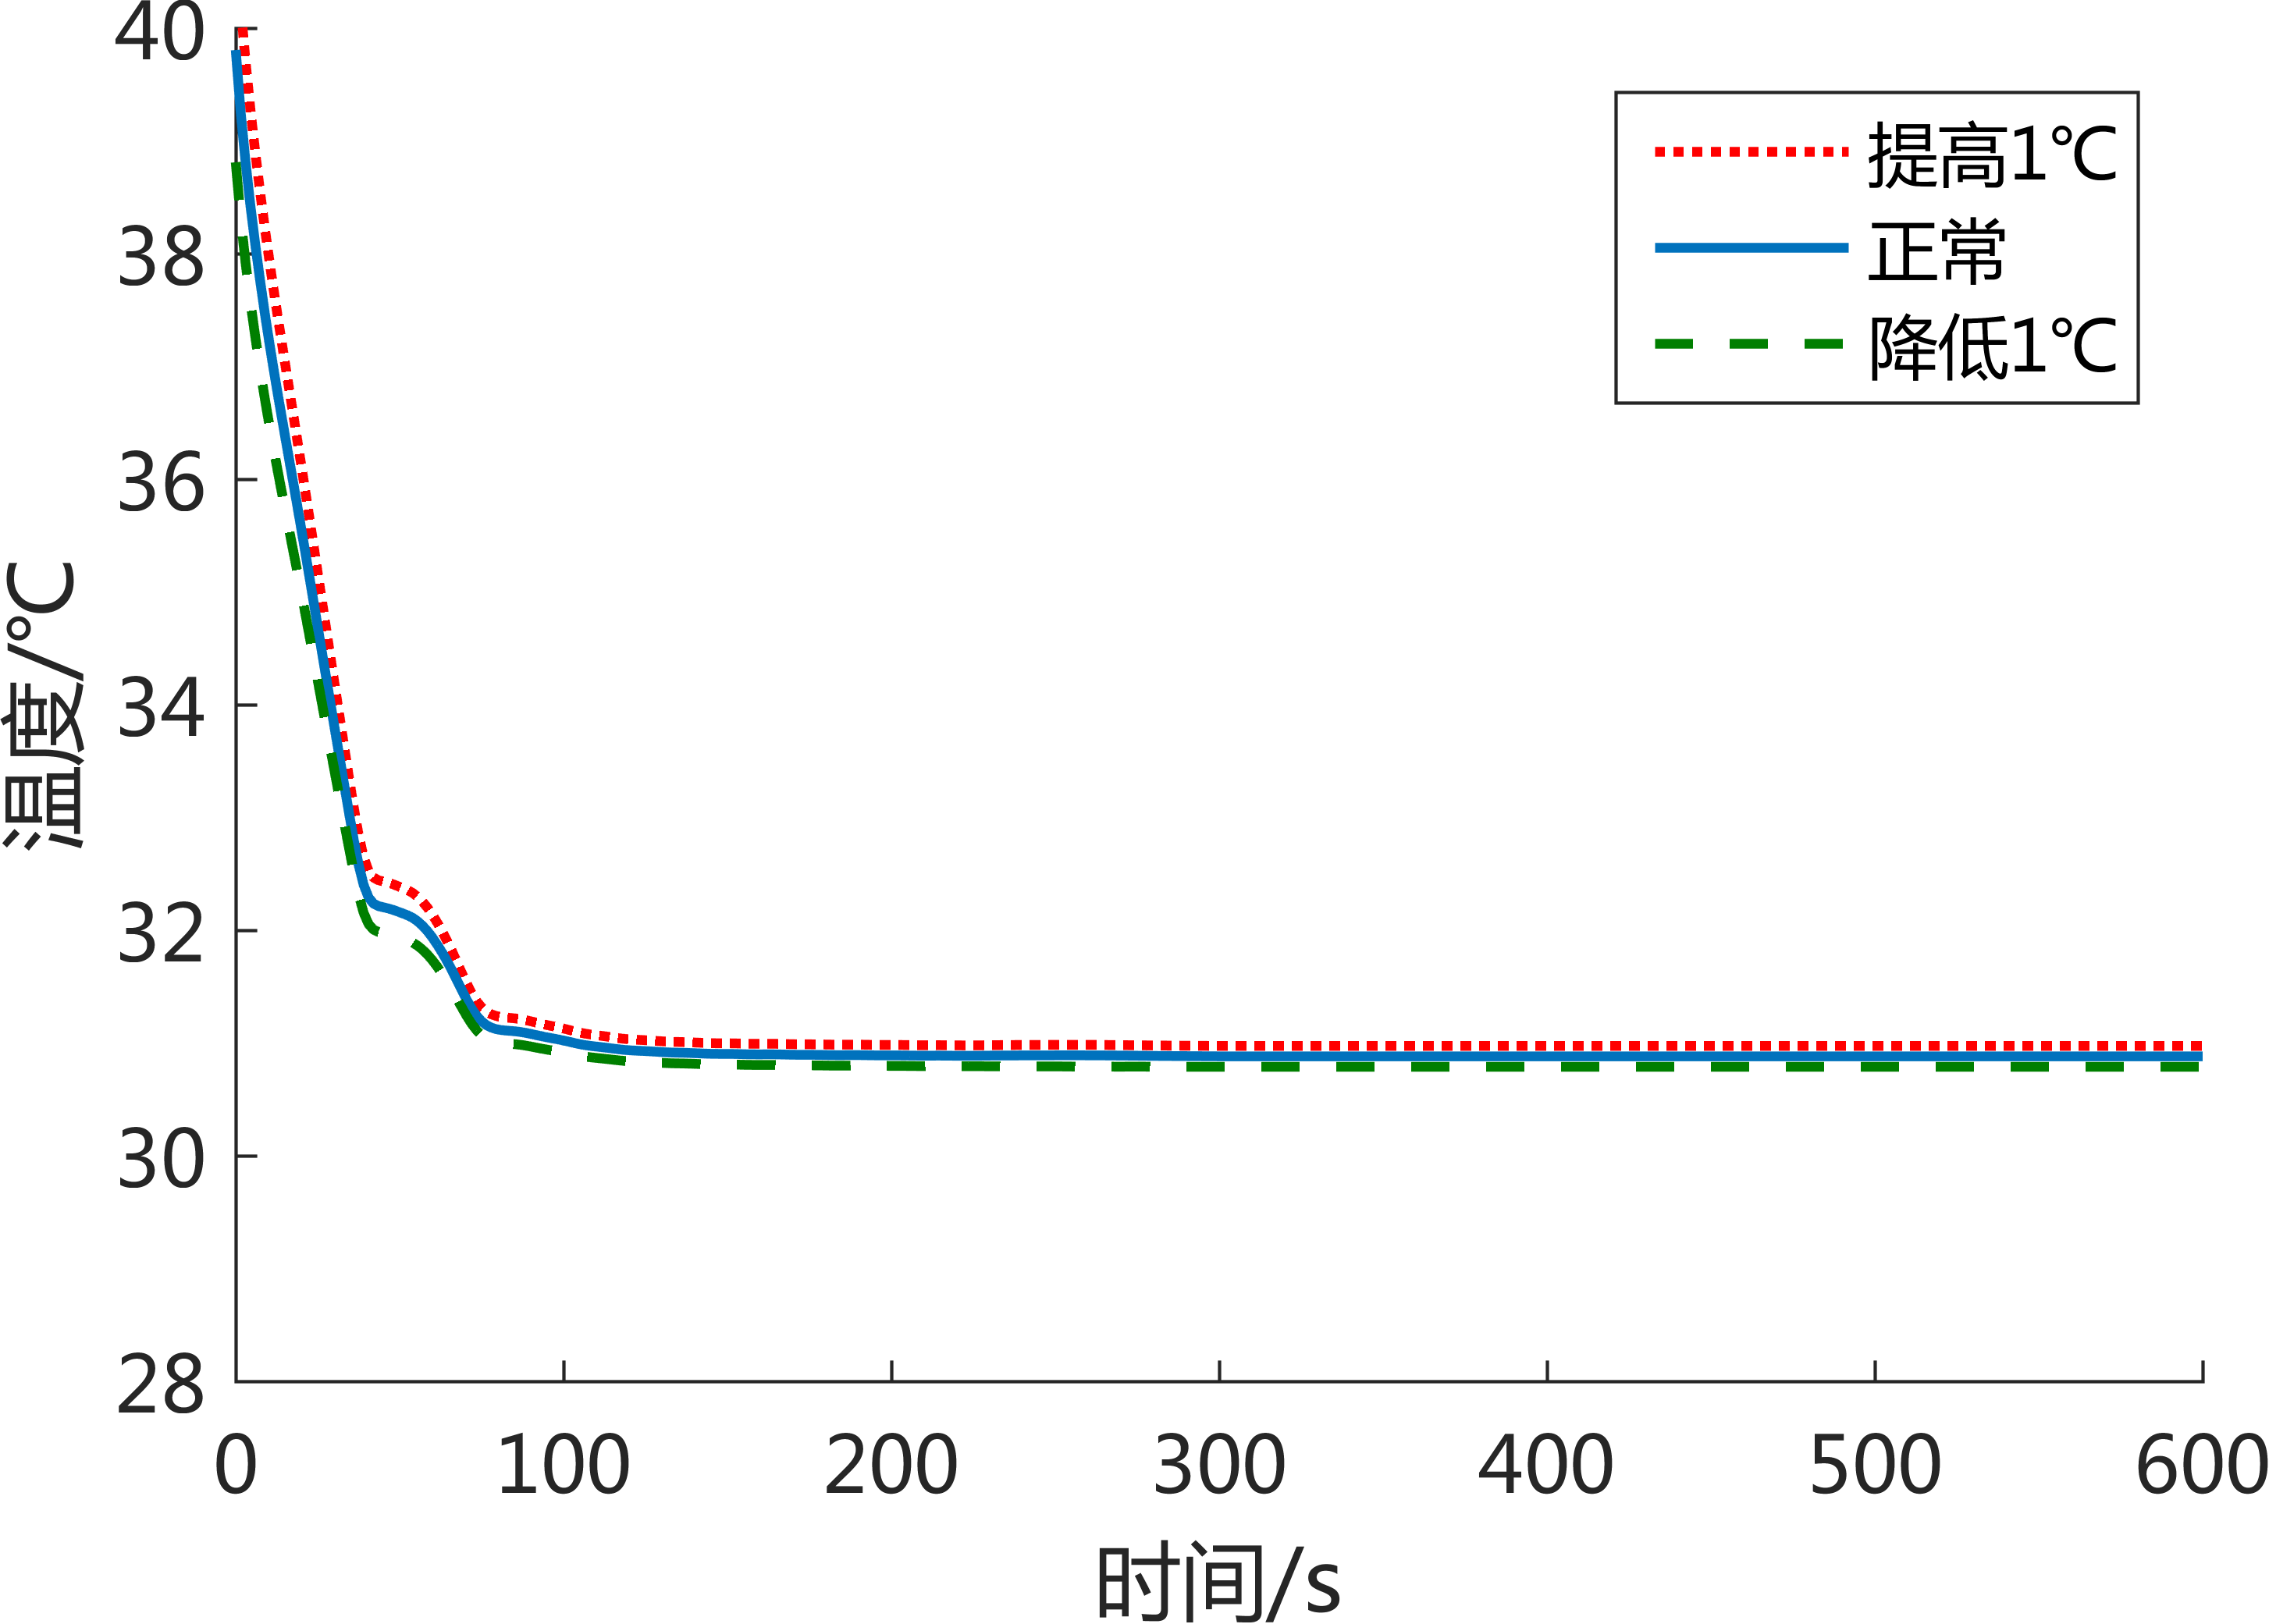
\includegraphics[width=0.4\textwidth]{compare/04.png}
		}
 		\bicaption[fig:Compare]{植物冠层仿真温度与实测温度变化曲线}{植物冠层仿真温度与实测温度变化曲线}{Fig}{Curve of the simulated and measured temperature at Section L}
 	\end{figure}
由\ref{fig:Compare}可知,在空气温度下降阶段,各测点的仿真值相比于对应实测值下降速率明显快,其主要原因是仿真模型是理想的密封环境,而实际温室存在不可避免的空气渗透问题。在稳定阶段两者基本一致,即各个截面的各测点位置的最终稳定温度基本一致。稳定阶段实测值仍会发生小范围内的波动,而仿真值则不会,其主要原因是仿真模型是理想的稳定环境,而实际温室中会存在各种各样不可避免的环境扰动,从而导致温度稳定后仍会发生一定的波动。变化过程中温度梯度也保持一致,即在截面2方向上,距离湿帘越近的位置空气温度下降越早,下降速率也较快,最终达到的稳定温度也较低,第1栋和第2栋温度基本一致,第3栋温度相对较高,且下降速度较慢。
	\begin{figure}[!htbp]
		\centering
		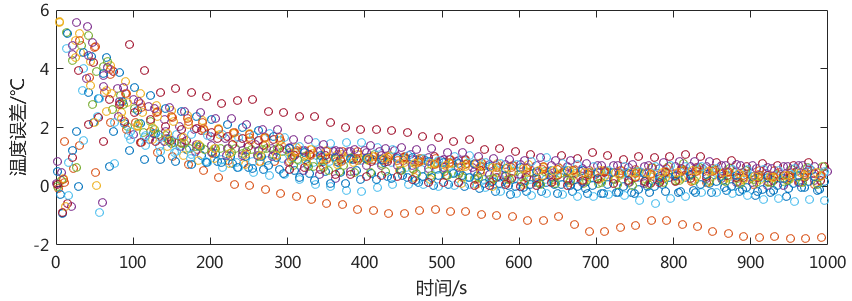
\includegraphics[width=0.8\textwidth]{21error.png}
		\bicaption[fig:Error]{仿真值与实测值绝对误差分布}{仿真值与实测值绝对误差分布}{Fig}{Distribution of absolute error between the simulated and measured temperature}
	\end{figure}
从风机开启至空气温度下降到稳定阶段,温室内所有测点的绝对误差,即实测值与仿真值之差,分布如\ref{fig:Error}所示。由图可知,误差较大的区域主要集中在空气温度快速下降阶段,其主要原因是温室仿真模型和实际温室的差异,即实际温室存在不可避免的空气渗透问题,导致实际情况下空气温度下降速率相较于仿真的理想状态略缓慢,由\ref{fig:Compare}也可观察到这一现象,从而导致在空气温度快速下降阶段误差较大。整个过程均方根误差为1.39℃,平均相对误差为2.63\%,稳定阶段均方根误差为0.53℃,平均相对误差为0.79\%。误差分析结果表明,仿真值和实测值虽存在一定的偏差,但整体温度场的分布和温度变化的趋势基本保持一致。因此,本文所建立的温室CFD仿真模型是有效的,仿真结果能够比较准确的显示温室气温的分布和变化。

\section{机械通风过程分析}
机械通风过程分析以实验条件为例进行分析,实验条件即为表6中的方案1条件,开启风机数量为10台,入口温度为30℃,温室长度为32 m,其它基本参数设置如表5所示。

\ref{fig:V2}所示为实验条件下机械通风过程中截面2的速度瞬态分布云图。从图中可以看出,受机械通风、热浮力共同作用,以及温室边界的限制,温室内气体流动可以看出明显的湍流现象。湿帘入口处空气流动较快,且速度变化较为剧烈,呈现明显的速度梯度,温室内部风速逐渐减弱,温室的上部和边角处速度较小。在机械通风的整个过程,外部空气从湿帘处进入温室从而带动温室内部的空气流动,首先会空气流会在温室内上下波动,达到稳定状态后在风机和湿帘的连线处形成一条空气流,并不断进行小范围内的上下波动。
	\begin{figure}[!htbp]
		\centering
		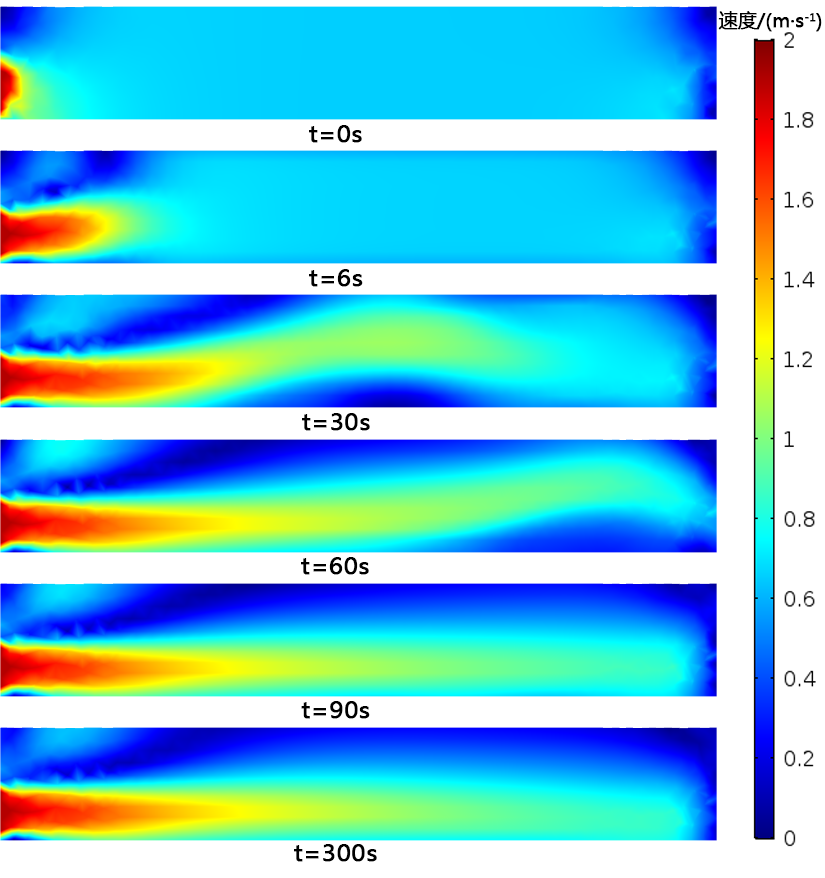
\includegraphics[width=0.5\textwidth]{22V2.png}
		\bicaption[fig:V2]{截面2速度瞬态分布云图}{截面2速度瞬态分布云图}{Fig}{Transient distribution of velocity at Section 2}
	\end{figure}
\ref{fig:VL}所示为实验条件下机械通风过程中截面L的速度瞬态分布云图。可以看出风机出口处空气流动也较快,也呈现出较为明显的速度梯度。另外可以观察到,受温室推拉门的影响,温室中部风速明显较低,且基本不发生变化,通风效果较差。
	\begin{figure}[!htbp]
		\centering
		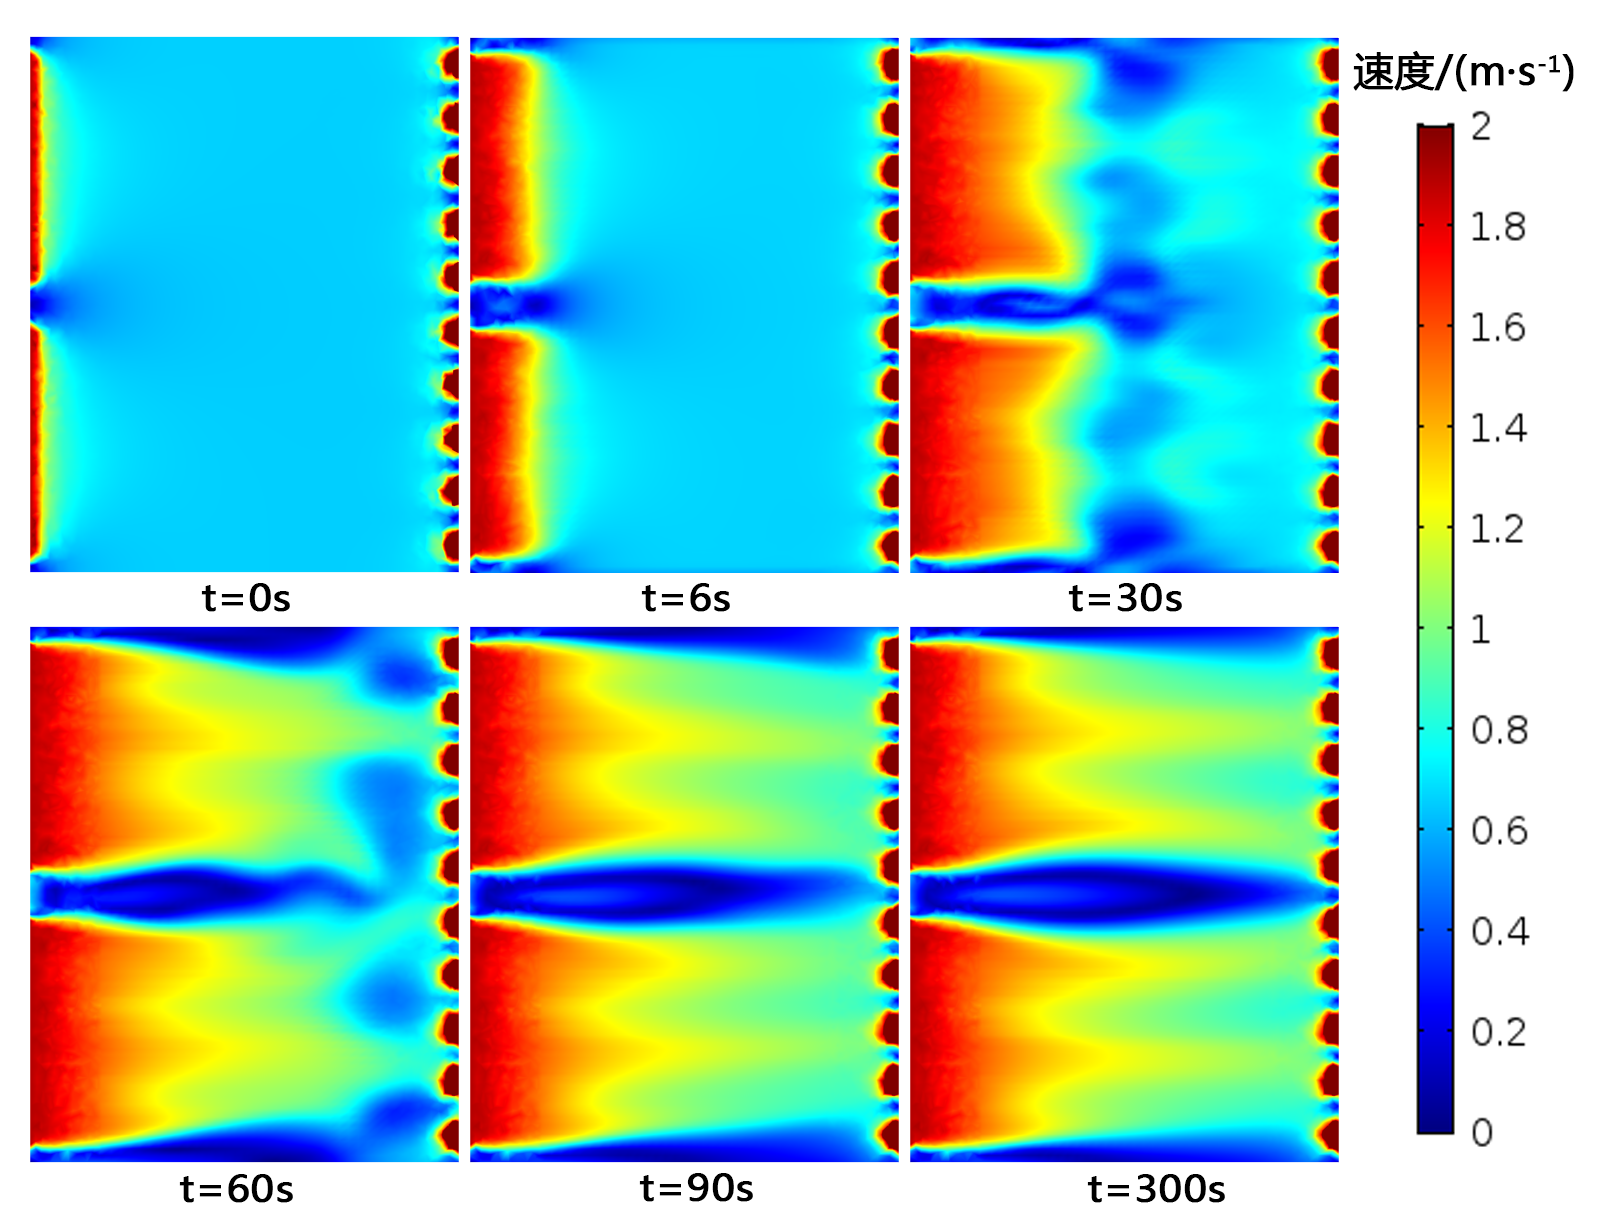
\includegraphics[width=0.8\textwidth]{23VL.png}
		\bicaption[fig:VL]{截面L速度瞬态分布云图}{截面L速度瞬态分布云图}{Fig}{Transient distribution of velocity at Section L}
	\end{figure}
\ref{fig:T2}所示为实验条件下机械通风过程中截面2的温度瞬态分布云图。从图中可以看出:整个通风过程中,地面附近温度相对较高,主要因为这些地方受到强烈的太阳辐射的影响;顶棚附近温度较高,主要因为受太阳辐射和热浮力的共同影响。同时还可以观察到机械通风过程中,风机将温室内热空气抽出产生负压,空气从湿帘处进入温室,经过湿帘将显热转化为潜热形成温度较低的冷空气,形成的冷空气在向前推进的过程中,冷空气会包裹温室内原有的暖空气形成温度漩涡,未及时推动的暖空气会被卷入其中,在冷空气流中不断进行热交换并向前移动,直至到达风机端处排出。
	\begin{figure}[!htbp]
		\centering
		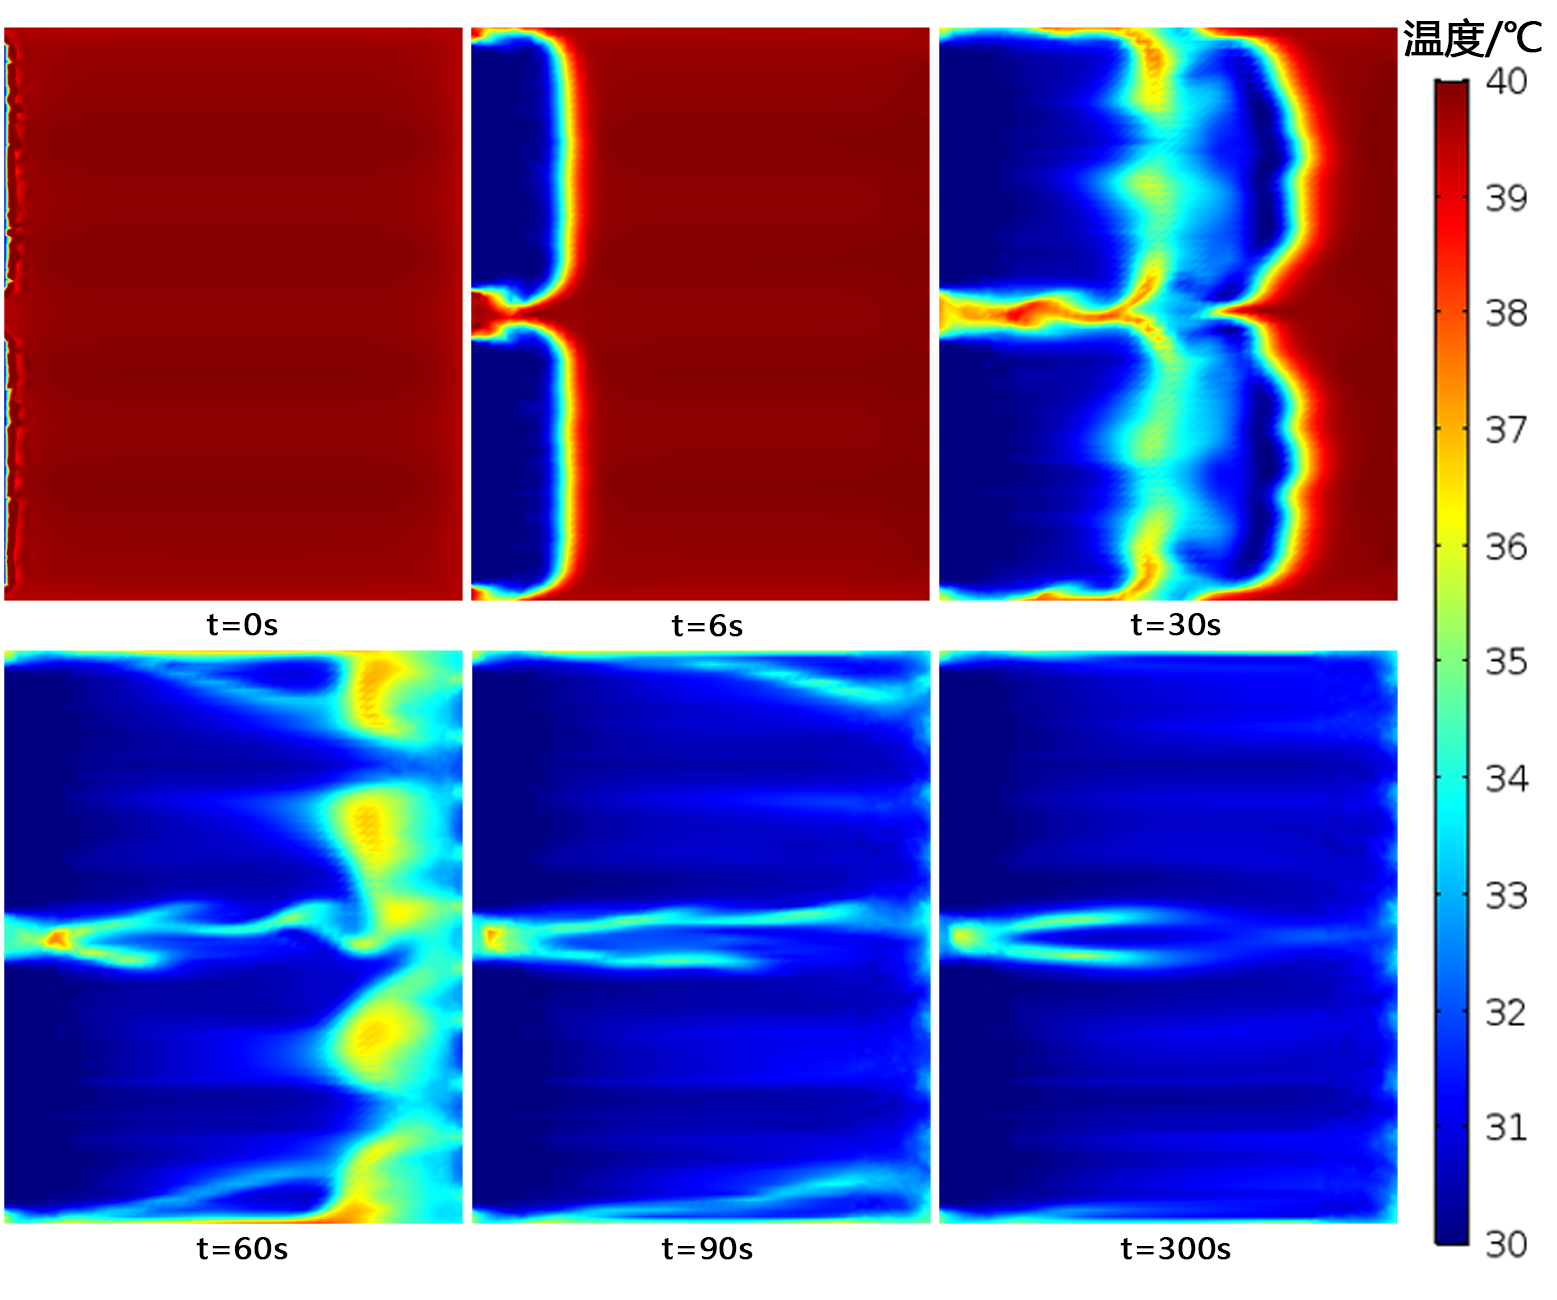
\includegraphics[width=0.5\textwidth]{24T2.png}
		\bicaption[fig:T2]{截面2温度瞬态分布云图}{截面2温度瞬态分布云图}{Fig}{Transient distribution of temperature at Section 2}
	\end{figure}
\ref{fig:VL}所示为实验条件下机械通风过程中截面L的温度瞬态分布云图。从图中可以看出:整个通风过程中,四周壁面附近温度相对较高,主要因为这些地方受到强烈的太阳辐射的影响。由于温度漩涡的存在,水平面上冷空气流在向前推进的过程中会产生断裂,由图28也可观察到这一现象的发生过程。由于气流将热空气携带至风机口处排出,同时受到风机处边界的阻碍,导致风机口处的空气温度相对较高。另外,由于温室中间推拉门的存在,形成了两套湿帘之间的不连续,从而使温室水平方向中间部分的通风效果较差,导致该区域的降温效果也较差。在\ref{fig:T2}和\ref{fig:TL}中还可以看出,受温室边界及热浮力的影响,温室各角落温度相对较高。
	\begin{figure}[!htbp]
		\centering
		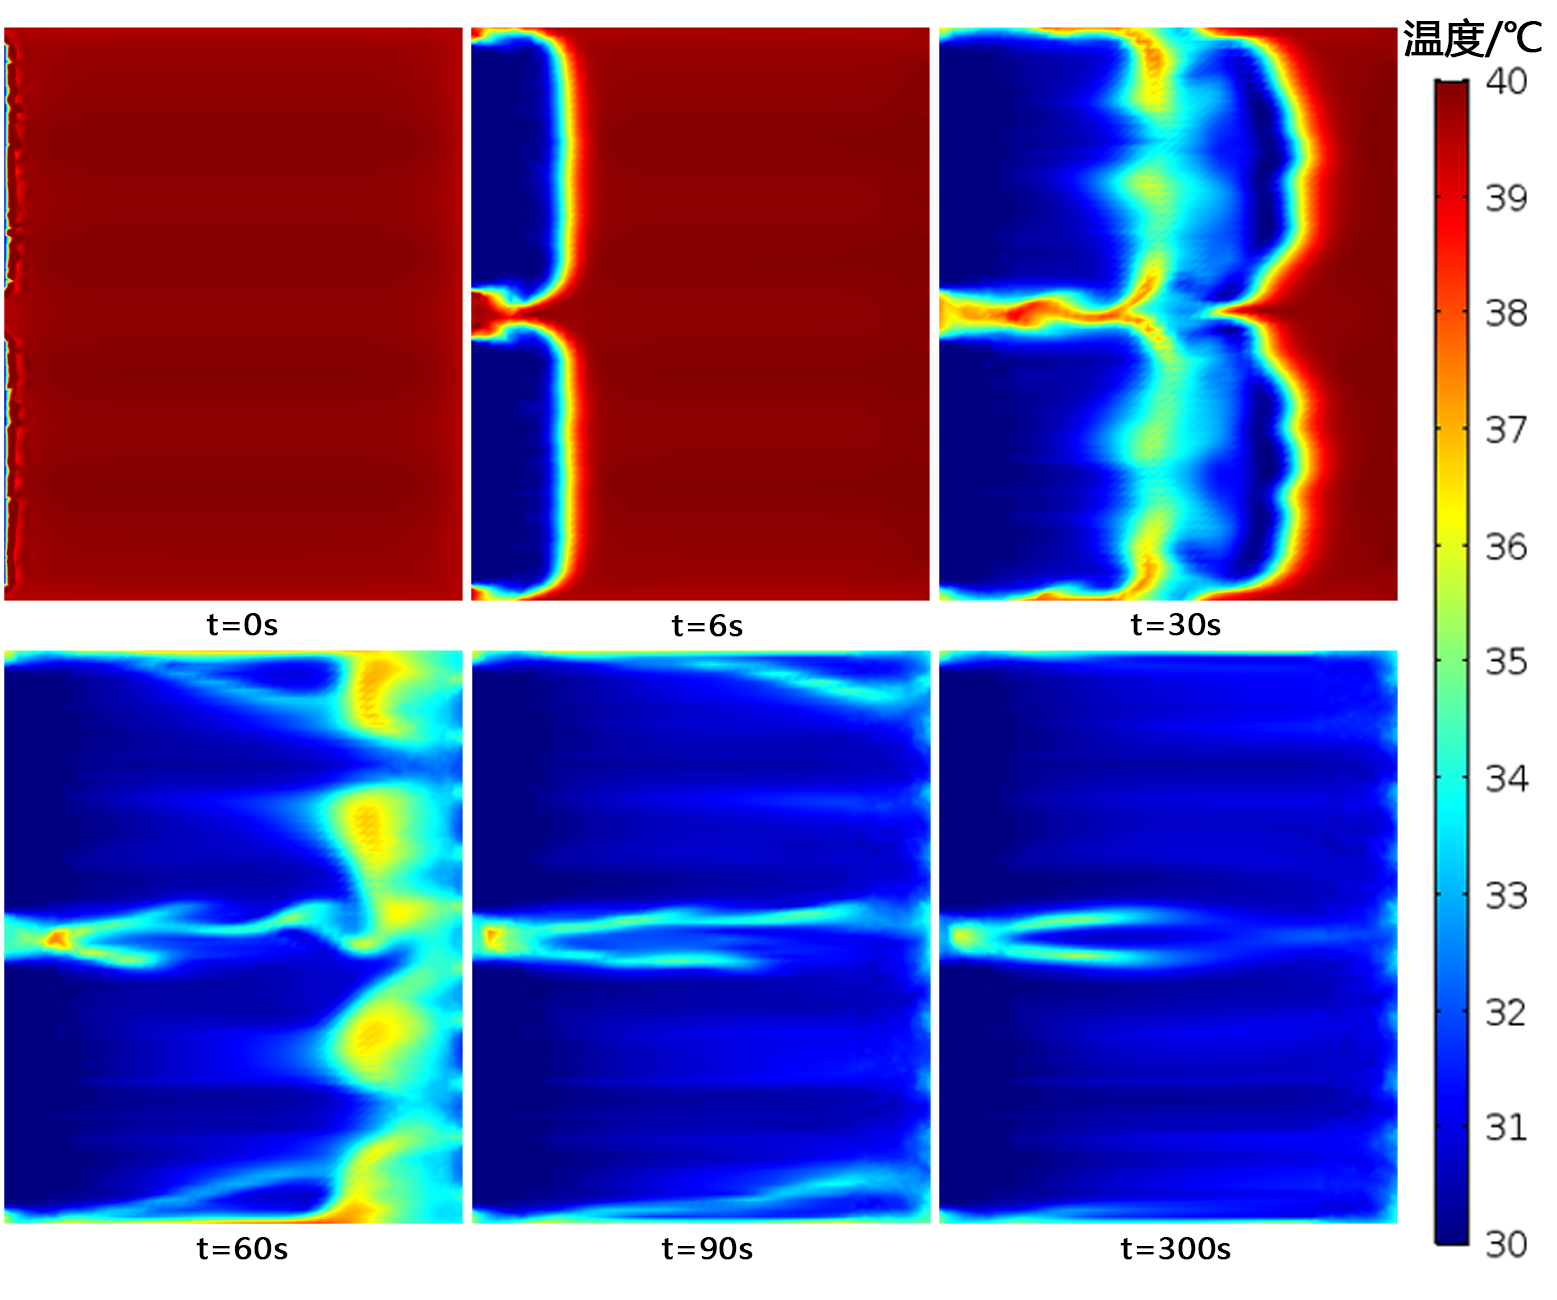
\includegraphics[width=0.8\textwidth]{25TL.png}
		\bicaption[fig:TL]{截面L温度瞬态分布云图}{截面L温度瞬态分布云图}{Fig}{Transient distribution of temperature at Section L}
	\end{figure}
\section{本章小结}
本章针对机械通风降温而带来的能源消耗、生产成本较高的问题,和温室面积大带来的监测点较多、监测成本较高的问题,建立温室CFD仿真模型,对温室机械通风过程进行分析,为温室优化结构参数和通风设备配置,为基于农业物联网的智能温室监测与控制系统提供优化的监测点位置选择和机械通风控制策略。

本章首先阐述分析了温室CFD仿真的概况和研究意义。然后对CFD仿真的理论基础进行了简单阐述,选择COMSOL Multiphysics多物理场仿真软件进行温室CFD仿真建模,并对温室仿真模型进行了几何建模、多物理场选择、边界条件设置、网格划分和求解。

为了验证仿真模型的有效性和可靠性,本章基于智能温室监测与控制系统进行了夏季温室机械通风实验,并详细说明了本次通风实验的实验方案和实验步骤,然后将实验结果和仿真结果进行了对比分析,验证了仿真模型瞬态和稳态计算的准确性和有效性。

最后本章基于已经验证的温室仿真模型对温室的机械通风过程进行了分析,得到了机械通风过程中温室内空气流动的规律和空气温度的分布和变化规律。

本章所建立的温室仿真模型虽然是针对本文实验温室建立,但是建立仿真模型的原理和方法是通用的,可针对任意温室修改几何模型和边界条件设置,重新划分网格即可进行仿真分析;同理,本文的模型虽然是针对夏季温室机械通风建立,但是可对边界条件进行一定的修改即可对其它条件下的温室稳态和瞬态过程进行分析。 %智能温室的实践与应用
%# -*- coding: utf-8-unix -*-
%%==================================================
%% chapter0.tex for SJTU Master Thesis
%%==================================================


\chapter{智能温室的实践与应用}
\label{chapter:Application}
温室CFD仿真模型建立完成后,需要借助其进行各种计算,得出不同的计算结果并进行分析,才能发挥出数值仿真的价值和优势。智能温室监测与控制系统实现后之后,需要在实践应用中对其有效性、准确性、可靠性和稳定性进行验证。本章通过温室CFD仿真模型及其结果分析,得出了智能温室系统监测点位置选择优化方案、机械通风参数优化方案和机械通风控制策略优化方案。

\section{监测点位置选择与优化}
温室生产面积通常较大,一般在1200 m2以上,为了能够有效监测温室整体的环境状态,监测系统通常需要布置大量密集的监测点和传感设备,从而导致监测硬件成本过高。因此,为了使用尽量少的监测点准确地反映温室整体的环境分布和变化,本文通过对温室CFD仿真模型的仿真结果进行分析,把握温室内环境的分布和变化规律,从而选择和优化智能温室系统的监测点位置。

不同的温室在不同的大环境下,室内环境分布差别很大,监测的关注点也有较大的差别,本文针对实验温室在夏季高温条件下需要机械通风的情况下的监测为例进行监测点的优化,其它温室和环境下,可以充分利用无线传感器的优势,对温室环境分布进行分析后优化监测点的位置。

农业生产主要关注植物冠层的空气温湿度分布和变化,因此空气温湿度监测点的位置首先可以确定在植物冠层,即截面L处。为了让监测系统更加有效地反映温室的整体环境状态,系统需要确定能够代表温室内平均水平的监测点,如图27和图29所示,温室第3栋受温室推拉门的影响空气温度明显高于其它区域,因此不适宜作为空气温湿度监测点;靠近湿帘和风机的位置由于通风时空气流动剧烈,容易对空气温湿度监测点产生较大的影响,因此也不适宜作为空气温湿度监测点;温室第1、2、4、5栋的中间位置空气温度分布较为均匀且空气流动较温和,本文认为较为适宜作为空气监测点。

对于土壤温湿度状态的监测,由于土壤的温湿度一般情况下分布均匀且变化缓慢,所以要求较低,选取温室的中心位置进行监测即可。对于光照强度的监测,只要不被温室内的作物或其它障碍物遮挡即可。

综合考虑,针对实验温室在夏季高温条件下需要机械通风情况下的监测,本系统选取第1、2、4、5栋的中间位置的植物冠层位置作为空气温湿度监测点,选取温室中心位置作为土壤温湿度和光照强度的监测点。此时,可以仅使用最少5个监测点即可获取温室内环境状态的整体平均分布和变化,有效地减少了监测点的布置数量和布置密集度,从而有效地降低了系统的监测成本。

\section{智能温室远程监测与控制系统应用}
本文设计并实现的基于农业物联网的智能温室监测与控制系统在实验温室,即上海市崇明区连栋塑料温室(东经121.74,北纬31.50),进行了实施运行。现场微型计算机如图30所示,协调器如\ref{fig:real:a}所示,路由器节点封装如\ref{fig:real:b}所示,终端节点封装如\ref{fig:real:c}所示。
\begin{figure}[!htp]
	\centering
    \subfigure[协调器]{
		\label{fig:real:a} 
		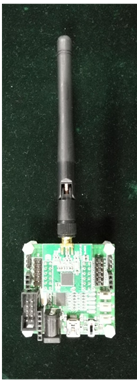
\includegraphics[height=4cm]{real/Cor.png}
	}
    \subfigure[路由器]{
		\label{fig:real:b} 
		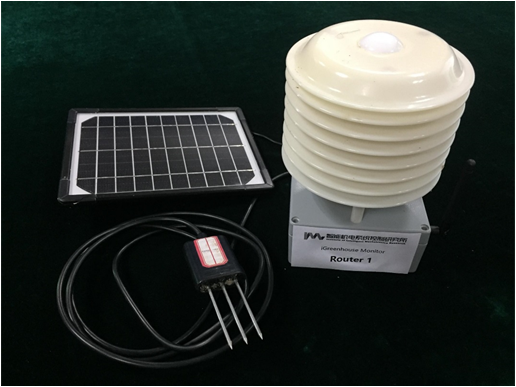
\includegraphics[height=4cm]{real/Router.png}
	}
	\subfigure[终端节点]{
		\label{fig:real:c}
		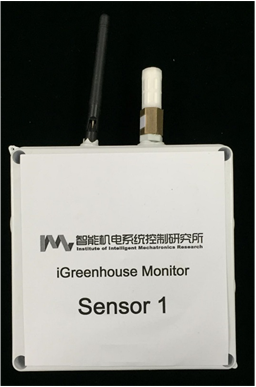
\includegraphics[height=4cm]{real/Node.png}
	}
    \bicaption[fig:real]{协调器、路由器封装和终端节点封装}{协调器、路由器封装和终端节点封装}{Fig}{Coordinator, router and endnode}
\end{figure}
根据通过仿真模型得到的温室监测点位置的优化结果,系统确定温室监测点布置方案:在实验温室内第1、2、4、5栋的中间位置各布置一个终端节点,用以监测温室内的空气温湿度分布和变化;在温室的中心位置布置一个路由器节点,用以监测温室内的土壤温湿度和光照强度,路由器节点还带有空气温湿度传感器,可以根据该节点的数据判断温室内最高温度的阈值,此外路由器节点还可以对无线传感器网络起到扩展的作用,从而能够监测更大范围内的温室,使距离较远的监测点能够接入网络,保证网络的覆盖范围和稳定性。此次实施运行,还在连栋塑料温室旁的9个单栋薄膜温室内各布置一个监测点,大部分为终端节点,少数为路由器节点,以保证网络的覆盖范围和稳定性。

系统运行期间运行稳定正常,无线传感器网络传输稳定可靠,温室内外数据采集准确正常,响应迅速,数据上传同步延迟在1s以内,控制指令下达准确迅速,延迟在5s以内,控制状态获取正常。数据中心工作正常,未发生慢查询或查询异常。云端WEB服务器及服务端程序运行稳定正常,接口响应迅速,数据返回完整准确。如图32所示为Android平台上的终端程序截图,IOS平台和WEB页面显示完全相同,程序运行正常,数据获取与解析正常。现场图像采集设备工作正常,视频延时在10 s以内,显示正常如\ref{fig:snapshot}所示。
	\begin{figure}[!htp]
		\centering
		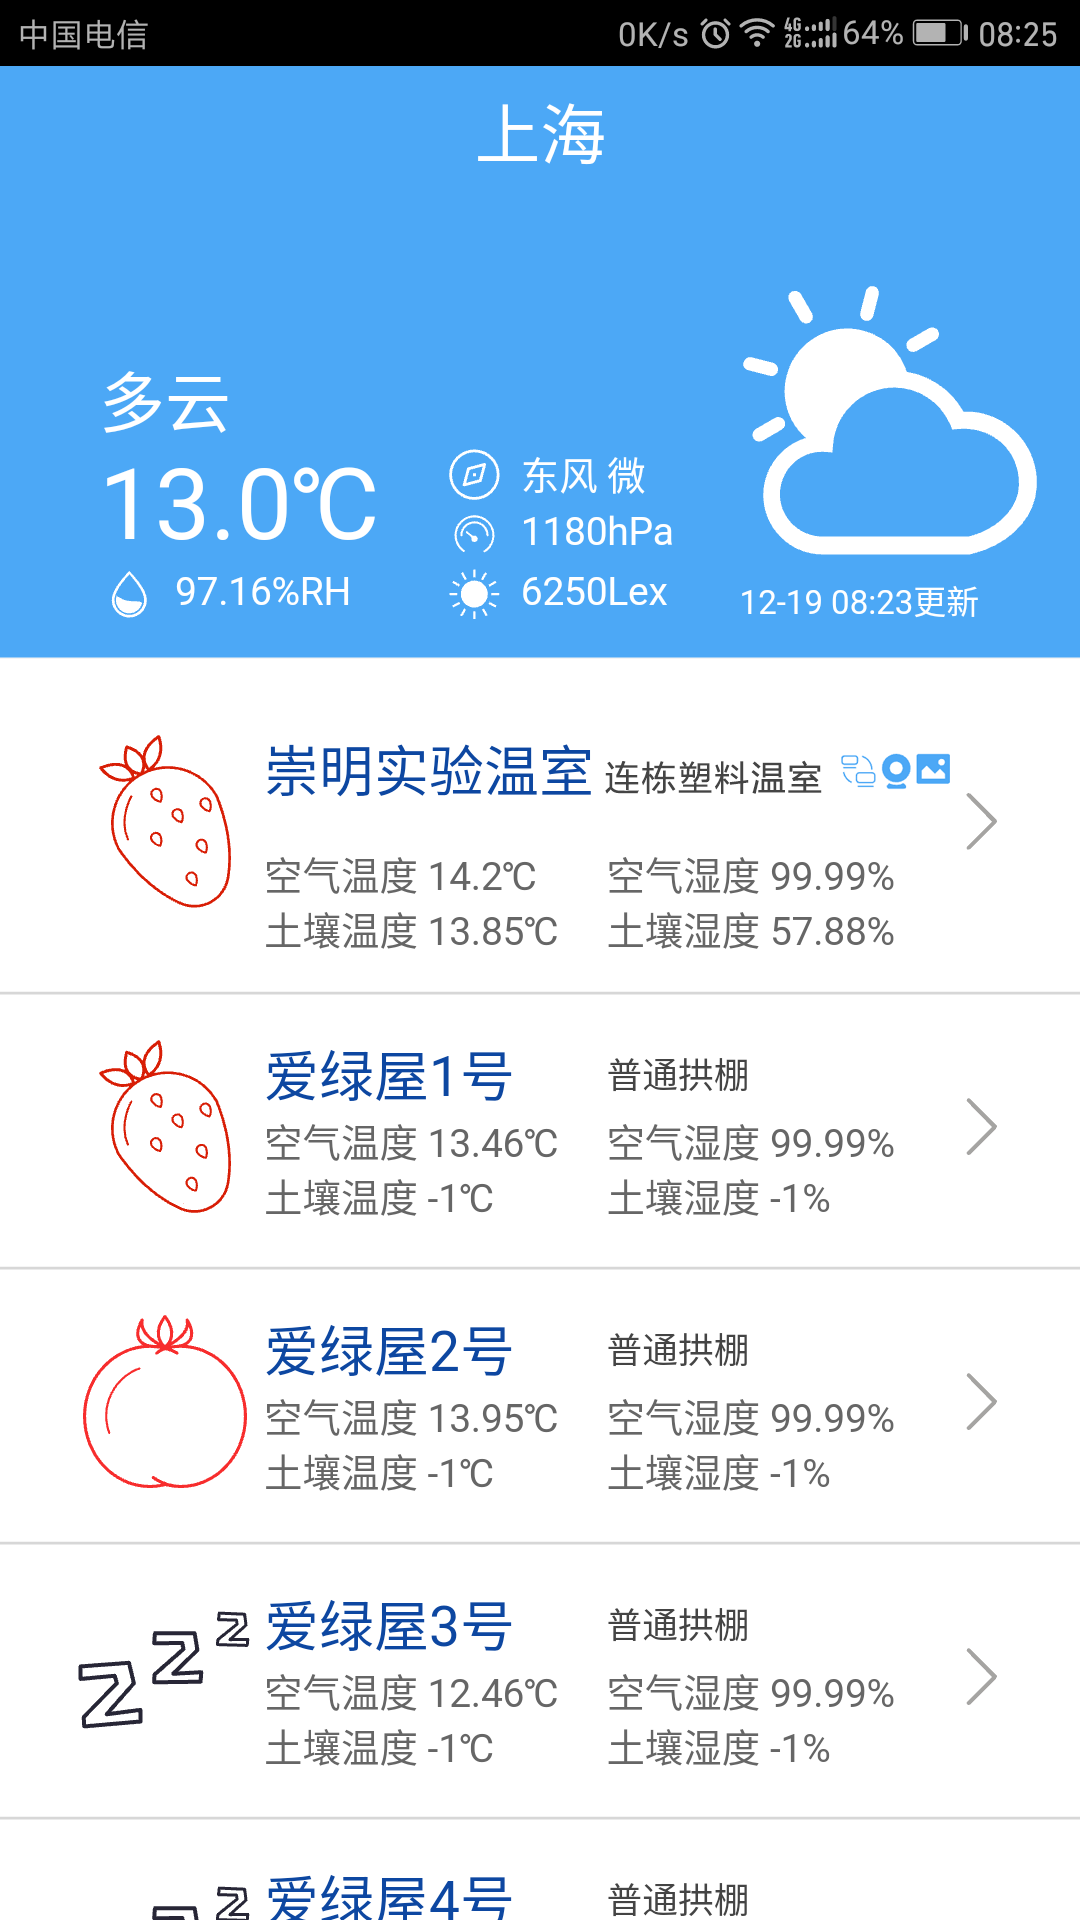
\includegraphics[width=0.19\textwidth]{android/home.png}
		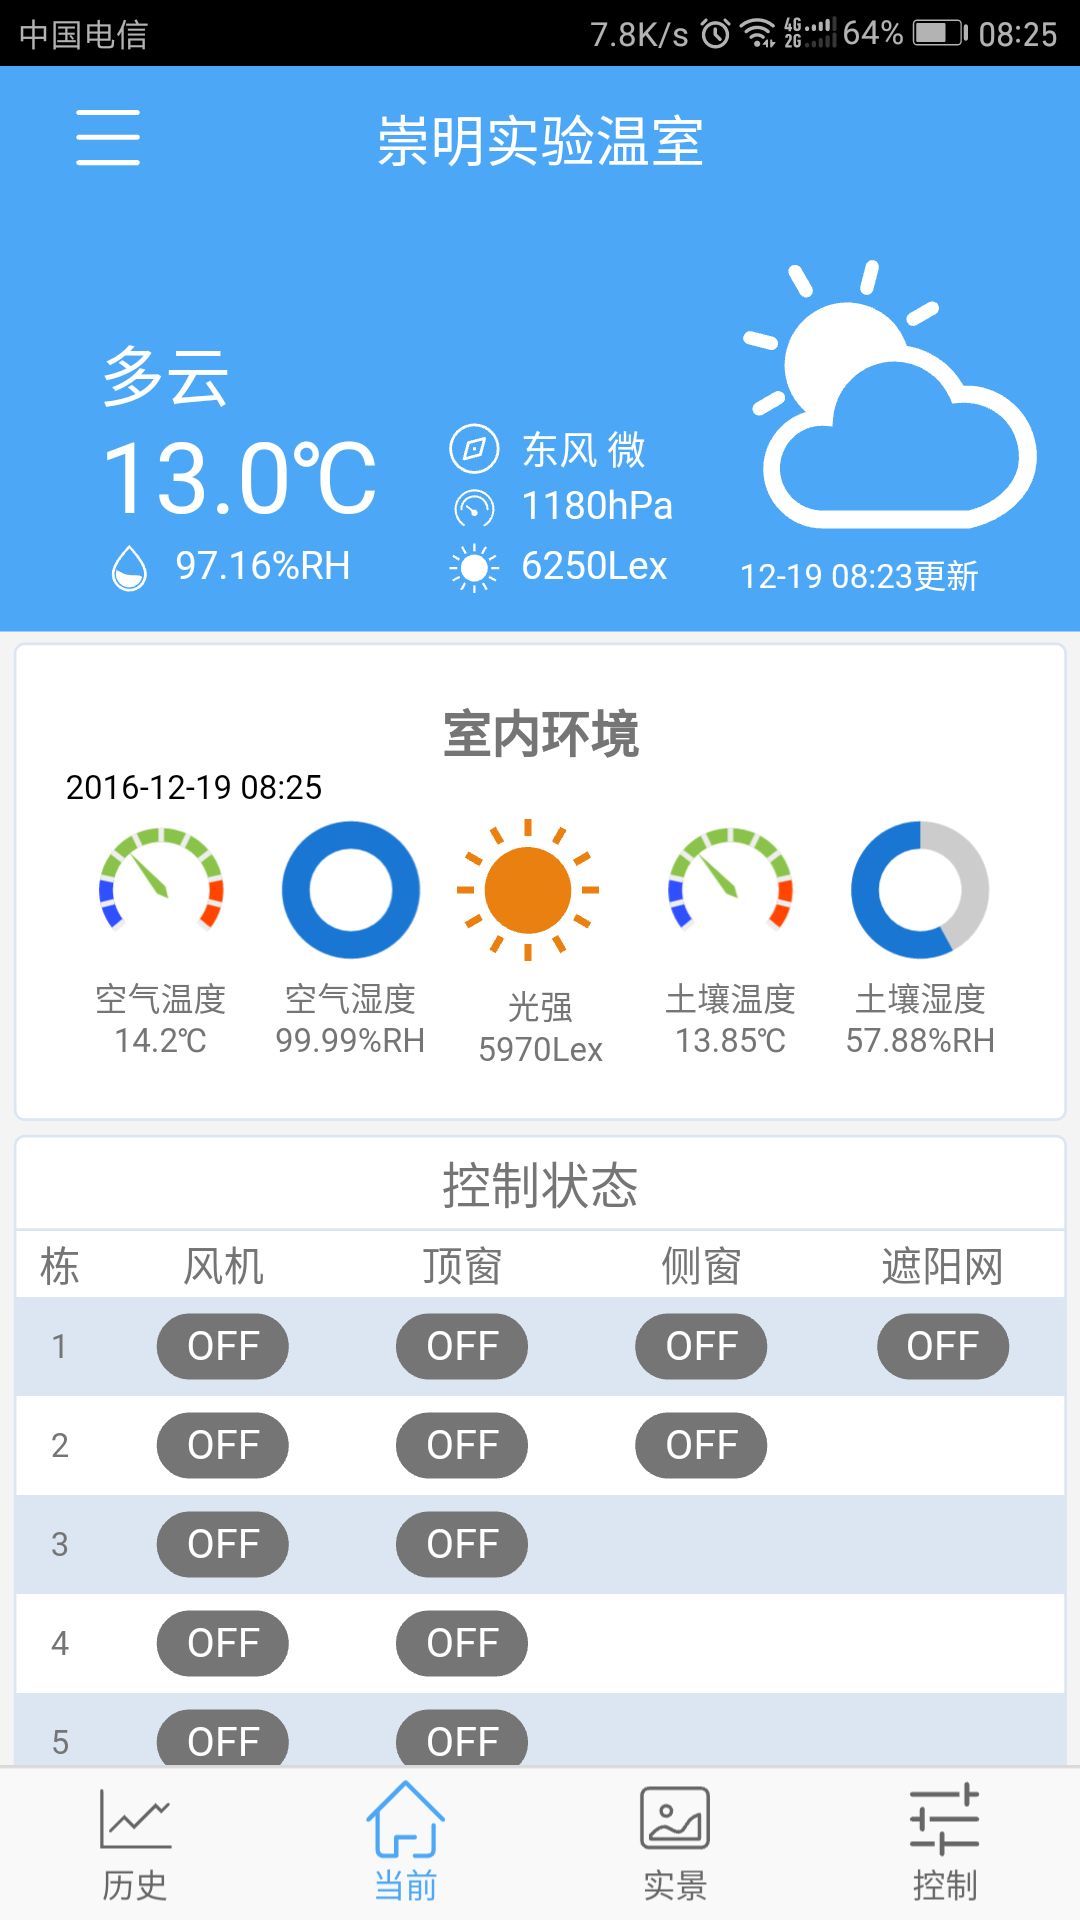
\includegraphics[width=0.19\textwidth]{android/detail.png}
		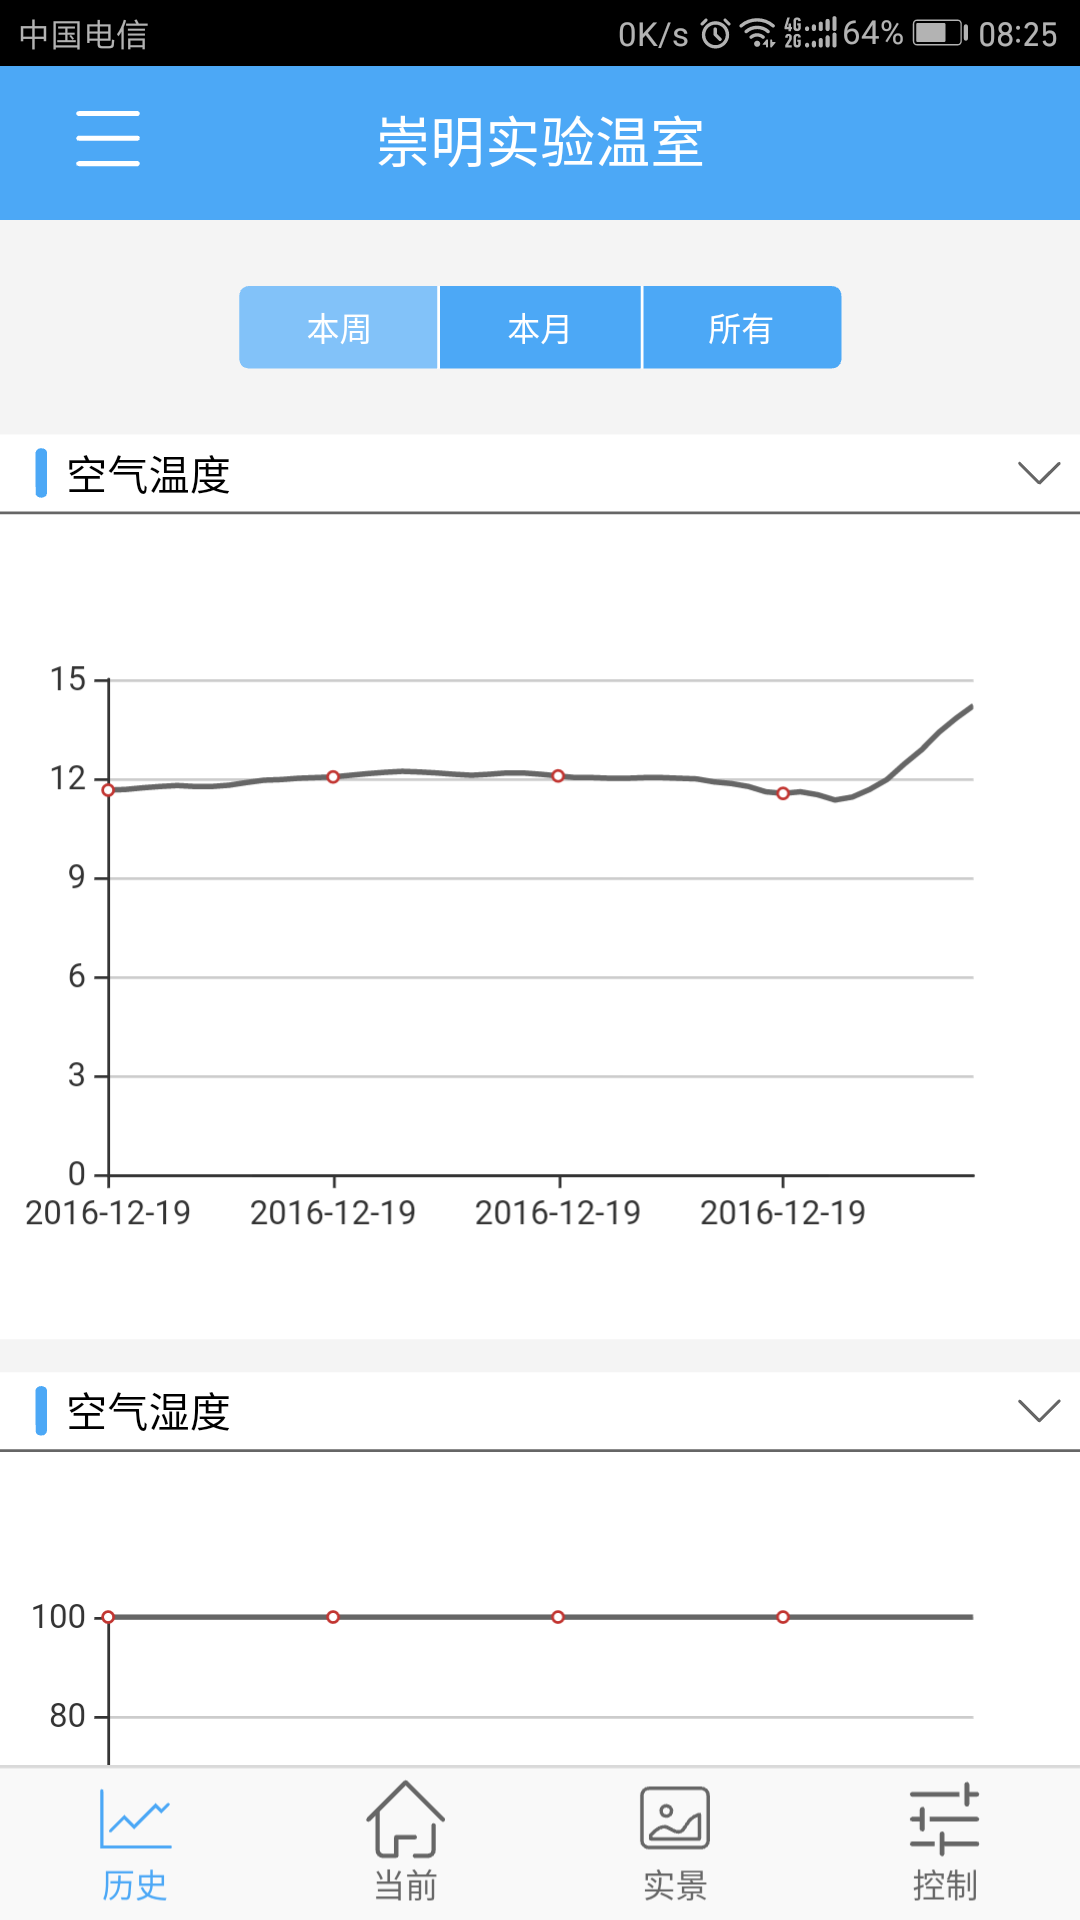
\includegraphics[width=0.19\textwidth]{android/history.png}
		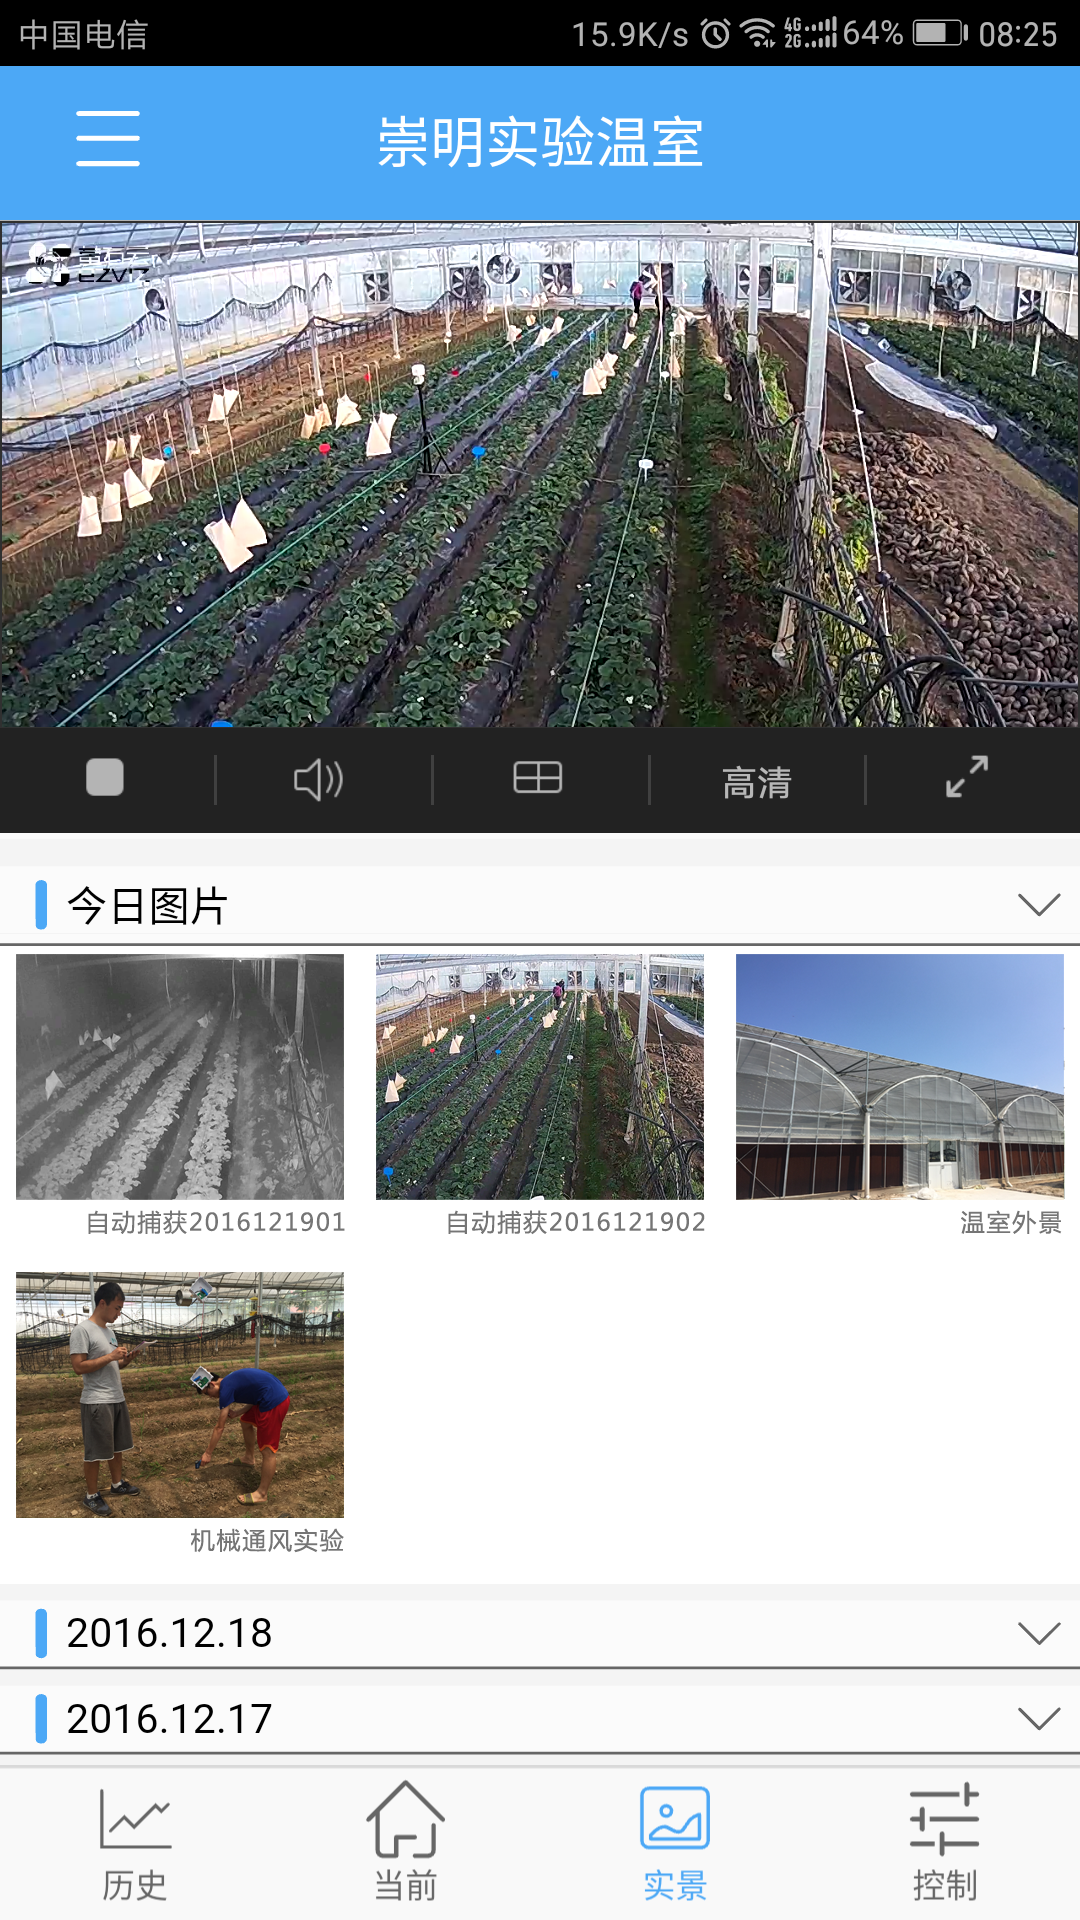
\includegraphics[width=0.19\textwidth]{android/video.png}
		\includegraphics[width=0.19\textwidth]{android/control.png}	
	    \bicaption[fig:snapshot]{终端程序截图}{终端程序截图}{Fig}{Snapshots of the terminal program}
	\end{figure}
现场测试运行结果表明,系统整体稳定可靠,符合预期设计要求和生产要求,可有效提高温室生产过程的科学管理水平。

\section{机械通风优化设计}
	\subsection{机械通风参数优化}
本文主要分析开启风机个数、入口温度、温室长度和环境温度变化(即相对于表5室内地面温度、薄膜壁面温度和薄膜顶棚温度变化)对于温室机械通风降温效果的影响。为分析这些因素的影响,本文控制不同因素变量的变化,共进行了12组仿真计算,各组的参数设置如\ref{tab:cases}所示,其它基本参数每组保持不变,详情如表5所示。
		\begin{table}[!htp]
  			\centering
  			\bicaption[tab:cases]{仿真方案参数设置}{仿真方案参数设置}{Table}{Parameters in different simulation cases}
  			\begin{tabular}{ccccc} \toprule
			方案编号 & 风机数量/个 & 入口温度/℃ & 温室长度/m & 环境温度变化/℃\\ \midrule
			1 & 10	 & 30 & 32 & 0\\
			2 & 6 & 30 & 32 & 0\\
			3 & 4 & 30 & 32 & 0\\
			4 & 2 & 30 & 32 & 0\\
			5 & 10 & 28 & 32 & 0\\
			6 & 10 & 29 & 32 & 0\\
			7 & 10 & 31 & 32 & 0\\
			8 & 10 & 30 & 40 & 0\\
			9 & 10 & 30 & 48 & 0\\
			10 & 10 & 30 & 100 & 0\\
			11 & 10 & 30 & 32 & 1\\
			12 & 10 & 30 & 32 & -1\\ \bottomrule
 			\end{tabular}
		\end{table}
	如\ref{fig:cases}所示为不同仿真方案下,植物冠层即截面L空气温度仿真平均值的变化曲线。
		\begin{figure}[!htp]
		\centering
		\subfigure[不同风机开启情况]{
			\label{fig:cases:a}
			\includegraphics[width=0.4\textwidth]{cases/01.png}
		}
		\subfigure[不同温室长度]{
			\label{fig:cases:b}
			\includegraphics[width=0.4\textwidth]{cases/02.png}
		}
		\subfigure[不同入口温度]{
			\label{fig:cases:c}
			\includegraphics[width=0.4\textwidth]{cases/03.png}
		}
		\subfigure[不同环境温度变化]{
			\label{fig:cases:d}
			\includegraphics[width=0.4\textwidth]{cases/04.png}
		}
 		\bicaption[fig:cases]{截面L不同方案下空气温度仿真平均值变化曲线}{截面L不同方案下空气温度仿真平均值变化曲线}{Fig}{Simulated average values of air temperature in different cases at section L}
 	\end{figure}
由\ref{fig:cases:a}可以看出开启风机数量对于温室内降温速度的影响较大,但是在一定范围内对于温室最终的稳定温度影响较小。随着开启风机数量的减少,温室内降温速度在一定程度上变慢,且稳定温度会略微升高。相较于开启10台风机时降温至稳定温度的时间,开启6台风机时约为其1.5倍,开启4台风机时约为其2.2倍,开启2台风机时约为其4.5倍。相较于开启10台风机时最终降温的稳定温度,开启6台风机时和4台风机时约升高0.3℃,开启2台风机时约升高0.7℃。根据这一现象,可以对温室机械通风设计时风机的配置和运行时开启风机的数量可以进行一定的优化,即在对降温速度要求不高的情况下,可适当减少风机的配置数量或开启风机的数量,降低机械通风硬件成本,同时可以降低运行成本和减少能耗;对于种植对温度较为敏感的作物的温室,可以在温度上升到过高之前提前开启风机,此时也可适当减少运行风机的数量达到相同的降温效果。

由\ref{fig:cases:b}可以看出,温室长度的增加会影响降温效果,不仅会增加降温时间,而且会提高稳定温度,但在一定范围内对降温效果的影响较小,对于降温时间的增加和稳定温度的提高都不是很明显,如仿真结果显示在温室长度增加50\%,即由32 m增加到48 m的情况下,最终可降低到的平均稳定温度仅升高约0.5℃,但此时单位面积上的机械通风能耗明显下降。根据这一现象,可以在温室设计之初对温室结构参数进行一定的优化,即在作物对温度不是特别敏感的情况下,可适当增加温室的长度,降低温室单位面积的机械通风能耗。

由\ref{fig:cases:c}可以看出,入口温度的降低对于降温速度的影响较小,但会显著影响温室降温最终可以达到的稳定温度。随着湿帘处入口温度的降低,稳定温度会随之明显降低,由仿真结果可知入口温度每降低1℃,稳定温度平均可降低0.9℃。根据这一现象可知,入口温度对于温室降温效果的影响较为显著,因此可通过降低入口温度的方式改善降温效果,一般情况下可以使用如抽取地下水浸湿湿帘、增加湿帘厚度等方式降低入口温度。

由\ref{fig:cases:d}可以看出,外界环境温度较小范围的改变,对于机械通风的降温效果影响较小。

	\subsection{机械通风策略优化}
	图34所示为不同控制策略下,植物冠层即截面L空气温度仿真平均值的变化曲线。策略1为开启10台风机持续工作;策略2为开启10台风机降温至稳态温度后关闭风机,待温度回升到一定程度后再次开启10台风机降温,为保证温室平均气温低于32℃,本文在温度回升至32.59℃时即再次开启风机进行降温;策略3为开启10台风机迅速降温至稳态温度后只保留4台风机开启维持降温效果。
	
	在长时间连续降温的过程中,开始阶段的快速降温的能耗可忽略,因此选取稳定阶段,即600 s以后的两个完整周期评价不同控制策略的效果,结果如表7所示。
		\begin{table}[!htp]
  			\centering
  			\bicaption[tab:strategies]{不同控制策略结果比较}{不同控制策略结果比较}{Table}{Comparison of results with different control strategies}
  			\begin{tabular}{cccc} \toprule
			参数 & 策略1 & 策略2 & 策略3\\ \midrule
			风机数量/个 & 10 & 10 & 4\\
			间歇比 & 1 & 0.53 & 1\\
			等效风机数量/个 & 10 & 5.3 & 4\\
			平均温度/℃ & 30.88 & 31.82 & 31.09\\
			最高温度/℃ & 30.88 & 32.59 & 31.09\\
			温度稳定性/℃ & <0.1 & <0.43 & <0.1\\ \bottomrule
 			\end{tabular}
		\end{table}
	由控制策略结果比较表可知:
	
策略1的降温效果和稳定性都是最好的,但是大量风机连续工作导致能源消耗过大,降温成本较高。

策略2温室的降温效果较差,和策略1相比平均温度升高0.94℃,稳定性也较差,但相较于策略1可降低约47\%的能源消耗。

策略3温室的降温效果略微变差,和策略1相比平均温度仅升高0.21℃,稳定性也较好,同时相较于策略1可降低60\%的能源消耗。

因此针对实验温室,选择策略2和策略3都能大幅降低能源消耗,而策略3从实现的简单和效果两方面都为较适宜的机械通风控制策略。

\section{本章小结}
本章首先通过对经过验证的温室CFD仿真模型的仿真结果进行分析,得到了针对实验温室在高温条件下需要机械通风情况下的监测点位置选择与优化方案。然后对本文设计并实现的基于农业物联网的智能温室监测与控制系统在实验温室内进行了实践与应用,并得到了良好的使用效果,验证了系统的稳定性和可靠性。最后,针对实验温室,通过仿真模型模拟了室外高温条件下的风机数量、温室长度、入口温度及环境温度变化等参数对机械通风降温效果的影响程度,并模拟了不同数量风机启闭控制的降温效果,为温室结构参数和通风设备配置的优化提供了参考,为控制系统提供了优化的夏季机械通风降温控制策略。该部分优化方案虽然针对实验温室进行,但是仍可为其它同类温室机械通风系统的优化设计和节能减排提供一定的参考。
 %结论

\appendix	% 使用英文字母对附录编号,重新定义附录中的公式、图图表编号样式
\renewcommand\theequation{\Alph{chapter}--\arabic{equation}}	
\renewcommand\thefigure{\Alph{chapter}--\arabic{figure}}
\renewcommand\thetable{\Alph{chapter}--\arabic{table}}
\renewcommand\thealgorithm{\Alph{chapter}--\arabic{algorithm}}

%% 附录内容。
%# -*- coding: utf-8-unix -*-
%% app2.tex for SJTU Master Thesis
%% based on CASthesis
%% modified by wei.jianwen@gmail.com
%% version: 0.3a
%% Encoding: UTF-8
%% last update: Dec 5th, 2010
%%==================================================

\chapter{Maxwell Equations}

选择二维情况,有如下的偏振矢量:
\begin{subequations}
  \begin{eqnarray}
    {\bf E}&=&E_z(r,\theta)\hat{\bf z} \\
    {\bf H}&=&H_r(r,\theta))\hat{ \bf r}+H_\theta(r,\theta)\hat{\bm
      \theta}
  \end{eqnarray}
\end{subequations}
对上式求旋度:
\begin{subequations}
  \begin{eqnarray}
    \nabla\times{\bf E}&=&\frac{1}{r}\frac{\partial E_z}{\partial\theta}{\hat{\bf r}}-\frac{\partial E_z}{\partial r}{\hat{\bm\theta}}\\
    \nabla\times{\bf H}&=&\left[\frac{1}{r}\frac{\partial}{\partial
        r}(rH_\theta)-\frac{1}{r}\frac{\partial
        H_r}{\partial\theta}\right]{\hat{\bf z}}
  \end{eqnarray}
\end{subequations}
因为在柱坐标系下,$\overline{\overline\mu}$是对角的,所以Maxwell方程组中电场$\bf E$的旋度:
\begin{subequations}
  \begin{eqnarray}
    &&\nabla\times{\bf E}=\mathbf{i}\omega{\bf B} \\
    &&\frac{1}{r}\frac{\partial E_z}{\partial\theta}{\hat{\bf
        r}}-\frac{\partial E_z}{\partial
      r}{\hat{\bm\theta}}=\mathbf{i}\omega\mu_rH_r{\hat{\bf r}}+\mathbf{i}\omega\mu_\theta
    H_\theta{\hat{\bm\theta}}
  \end{eqnarray}
\end{subequations}
所以$\bf H$的各个分量可以写为:
\begin{subequations}
  \begin{eqnarray}
    H_r=\frac{1}{\mathbf{i}\omega\mu_r}\frac{1}{r}\frac{\partial
      E_z}{\partial\theta } \\
    H_\theta=-\frac{1}{\mathbf{i}\omega\mu_\theta}\frac{\partial E_z}{\partial r}
  \end{eqnarray}
\end{subequations}
同样地,在柱坐标系下,$\overline{\overline\epsilon}$是对角的,所以Maxwell方程组中磁场$\bf H$的旋度:
\begin{subequations}
  \begin{eqnarray}
    &&\nabla\times{\bf H}=-\mathbf{i}\omega{\bf D}\\
    &&\left[\frac{1}{r}\frac{\partial}{\partial
        r}(rH_\theta)-\frac{1}{r}\frac{\partial
        H_r}{\partial\theta}\right]{\hat{\bf
        z}}=-\mathbf{i}\omega{\overline{\overline\epsilon}}{\bf
      E}=-\mathbf{i}\omega\epsilon_zE_z{\hat{\bf z}} \\
    &&\frac{1}{r}\frac{\partial}{\partial
      r}(rH_\theta)-\frac{1}{r}\frac{\partial
      H_r}{\partial\theta}=-\mathbf{i}\omega\epsilon_zE_z
  \end{eqnarray}
\end{subequations}
由此我们可以得到关于$E_z$的波函数方程:
\begin{eqnarray}
  \frac{1}{\mu_\theta\epsilon_z}\frac{1}{r}\frac{\partial}{\partial r}
  \left(r\frac{\partial E_z}{\partial r}\right)+
  \frac{1}{\mu_r\epsilon_z}\frac{1}{r^2}\frac{\partial^2E_z}{\partial\theta^2}
  +\omega^2 E_z=0
\end{eqnarray}


\backmatter	% 文后无编号部分 

%% 参考文献
\printbibliography[heading=bibintoc]

%% 致谢、发表论文、申请专利、参与项目、简历
%% 用于盲审的论文需隐去致谢、发表论文、申请专利、参与的项目
\makeatletter

%%
% "研究生学位论文送盲审印刷格式的统一要求"
% http://www.gs.sjtu.edu.cn/inform/3/2015/20151120_123928_738.htm

% 盲审删去删去致谢页
\ifsjtu@review\relax\else
  %# -*- coding: utf-8-unix -*-
\begin{thanks}

提笔写下这段致谢辞,才惊觉自己即将真正离开,人生亦从此开始新的篇章。尽管不舍,却更珍惜,因为我的生命中有那么多可爱的人值得感激。他们使我的大学生活充满了色彩,无论收获、遗憾,对我来说都是值得珍藏的记忆。“享其实者思其树,饮其流者怀其源,学其成者念吾师”,在此论文完成之际,谨向我尊敬的指导老师黄震宇老师致以诚挚的谢意和崇高的敬意。黄老师不仅在学业上言传身教,而且以其高尚的品格给我以情操上的熏陶。本文的写作更是直接得益于他的悉心指点,从论文的选题到体系的安排,字句的斟酌,无不凝聚着他的心血。师恩重于山,无法用言语形容感激,惟愿师生情谊一生延续。在此还要感谢符凌峰,朱森林,常歌等师兄师弟在系统硬件上给予我无私的帮助,帮助我顺利的完成硕士课题。

感谢上海交通大学对我的培养,学校的培养让我学到了专业的科学文化知识,同时也提升了我的多方面的能力,塑造了我的人格,使我在未来的人生道路上能够更加信心百倍的走下去。
感谢我的父母,我的家人。焉得谖草,言树之背,养育之恩,无以回报。你们始终如一的支持和关爱是我人生道路不断前进的强大动力,教我学会坚强、勇敢,使我在磨砺中得到成长。祝你们永远健康快乐,这是我最大的心愿和牵挂。

在此,祝老师同学们,以及所有关心我的人和我所关心的人身体健康,工作顺利,心情愉快,幸福平安!
\end{thanks}
 	  %% 致谢
\fi

  % 盲审论文中,发表学术论文及参与科研情况等仅以第几作者注明即可,不要出现作者或他人姓名
\ifsjtu@review\relax
  %# -*- coding: utf-8-unix -*-

\begin{publications}{99}
    \item\textsc{第一作者}. {中文核心期刊论文}, 2007.  
    \item\textsc{第一作者}. {EI国际会议论文}, 2006.
\end{publications}

  %# -*- coding: utf-8-unix -*-

\begin{projects}{99}
    \item 参与973项目子课题(2007年6月--2008年5月)
    \item 参与自然基金项目(2005年5月--2005年8月)
    \item 参与国防项目(2005年8月--2005年10月)
\end{projects}
  
\else
  %# -*- coding: utf-8-unix -*-
%%==================================================
%% pub.tex for SJTUThesis
%% Encoding: UTF-8
%%==================================================

\begin{publications}{99}
    \item\textsc{黄震宇, 高浩天, 朱森林, 赵春宇, 蔡春花}. {南方连栋塑料温室夏季机械通风优化设计}[J]. 农业机械学报, 已录用.
    \item\textsc{高浩天, 朱森林, 常歌, 符凌峰, 黄震宇}. {基于农业物联网的智能温室系统架构与实现}[J]. 农机化研究, 已录用.
    \item\textsc{李腾, 高浩天, 赵春宇, 朱成刚, 黄震宇}. {种子风力筛选机分离室内气固两相流仿真与优化}[J]. 农机化研究, 2016,07:85-89.
    \item\textsc{符凌峰, 赵春宇, 黄震宇, 高浩天}. {基于ZigBee技术的连栋温室低功耗环境监测系统设计}[J]. 传感器与微系统, 2016, 08:74-76+79.
\end{publications}
	      %% 发表论文
  %# -*- coding: utf-8-unix -*-
%%==================================================
%% projects.tex for SJTUThesis
%% Encoding: UTF-8
%%==================================================

\begin{projects}{99}
    \item 973项目“XXX”
    \item 自然基金项目“XXX”
    \item 国防项目“XXX”
\end{projects}
  %% 参与的项目
\fi

% %# -*- coding: utf-8-unix -*-
\begin{patents}{99}
    \item 第一发明人,“永动机”,专利申请号202510149890.0
\end{patents}
	  %% 申请专利
% \include{tex/resume}	  %% 个人简历

\makeatother

\end{document}
